\documentclass[a4paper,12pt,utf8x,notitlepage]{article}

%%%%%%%%%%%%%%%%
%                              		  %
%  Packages and page geometry  %             
%                              		  %             
%%%%%%%%%%%%%%%%

%------------------------------------> Setting language
\usepackage[english, brazil]{babel}
\usepackage[utf8]{inputenc}
\usepackage[T1]{fontenc}
\usepackage{subfigure}
\usepackage{enumerate}

%------------------------------------> To enrich layouts 
\usepackage{amssymb,amsmath,amsthm} %  equations
\usepackage[ruled,vlined]{algorithm2e}     %  algorithms
\usepackage{minitoc, footmisc} 		     %  pages

%------------------------------------> To enrich code layout 
\usepackage{helvet, courier, type1cm}
\usepackage{listings}                   

%------------------------------------> To enrich figures
\usepackage{graphicx}
\usepackage[small]{caption} % for figures legends   
\graphicspath{{./figuras/}} % Default path

\usepackage{epstopdf}
\usepackage{pdfpages}

%------------------------------------> Defining colors
\usepackage{color} 
\definecolor{blackgreen}{rgb}{0,0.4,0}
\definecolor{gray}{gray}{0.3}
%\definecolor{blue}{rgb}{0,0,0.5}
\definecolor{green}{rgb}{0,0.5,0}
\definecolor{lightgreen}{rgb}{0,0.6,0}
\definecolor{purple}{rgb}{0.5,0,0.5}
\definecolor{darkred}{rgb}{0.5,0,0}
\definecolor{dkgreen}{rgb}{0,0.6,0}
\definecolor{mauve}{rgb}{0.58,0,0.82}
\definecolor{orange}{rgb}{1,0.5,0}


%------------------------------------> To enrich annexes 
\usepackage{appendix}

%------------------------------------> Changing default geometry layout
\usepackage{geometry}
\usepackage{setspace}
\addtolength{\hoffset}{-0.3cm}
\addtolength{\voffset}{-.5cm}
\addtolength{\textheight}{1.5cm}
\addtolength{\textwidth}{0.8cm}

%------------------------------------> Using fancy features for header and footpage 
\usepackage{fancyhdr}

%------------------------------------> To create hyperlinks
\usepackage[colorlinks=true, linkcolor=blue, citecolor=blue, urlcolor=blue]{hyperref} %, breaklinks=true


% Para usar matlab2tickz
\usepackage{pgfplots}
% and optionally (as of Pgfplots 1.3):
\pgfplotsset{compat=newest}
\pgfplotsset{plot coordinates/math parser=false}
%\RequirePackage[demo]{graphicx} 

%%%%%%%%%%%%%%%%%%%%%%%%%%%%%%%%%
%                               %
%  Some commands/configuration  %             
%                               %             
%%%%%%%%%%%%%%%%%%%%%%%%%%%%%%%%%

% Formating code typeset structure
\lstset{language=MATLAB, %C
%
basicstyle=\ttfamily\scriptsize,        % code font size
keywordstyle=\color{red}\textbf,	% key words style
commentstyle=\color{blue},		% comments style
%
% numbers=left,                   	% where to put line numbers
% numberstyle=\ttfamily\scriptsize, 	% line nuimbers style
% numberblanklines=false,			
%
captionpos=t,                   % put legend under the text
frame=TB,	                 
%
showspaces=false,               % show spaces
showstringspaces=false,         % show characters
showtabs=false,                 % show tabulation with characters
tabsize=4,	                % tabulation size
%
moredelim=[s][\color{blackgreen}]{'}{'},
moredelim=[s][\color{blackgreen}]{"}{"},
}

%%%%%%%%%%%%%%%%%%%%%%%%
%                      %
%  Personal hot keys   %
%                      %
%%%%%%%%%%%%%%%%%%%%%%%%

\newcommand{\tens}[1]{#1}
\providecommand{\vect}[1]{\mbox{\boldmath${#1}$}}%$
\newcommand{\argmin}[1]{\underset{#1}{\operatorename{argmin}}}
\newcommand{\diag}{\mathop{\mathrm{diag}}}
\newcommand{\norm}[1]{\ensuremath{\left\lVert #1 \right\rVert}}

\newcommand{\TODO}[1]{\textcolor{red}{\large TODO:}\textcolor{purple}{[#1]~}}
\newcommand{\HRule}{\rule{\linewidth}{0.5mm}}
\newcommand{\Lagr}{\mathcal{L}}

\renewcommand{\frame}[1]{\ensuremath{\Psi_{#1}}}        %frame \Psi_{\uppercase{#1}}
\newcommand{\R}[1]{\ensuremath{\mathbb{R}^{#1}}}        %R for real
\newcommand{\Id}[1]{\ensuremath{\tens{I}_{#1}}}         %Identity matrix
\newcommand{\tp}{\ensuremath{^{\mathsf{T}}}}		%transpose
\newcommand{\ft}[2]{\ensuremath{_{#1,#2}}} 		%from to
\newcommand{\rt}[1]{\ensuremath{^{#1}}}			%relative to	transpose
\newcommand{\HM}{\ensuremath{\tens{H}}}			%homogenous matrix
\newcommand{\Rot}{\ensuremath{\tens{R}}}		%rotation matrix
\newcommand{\homo}[1]{\ensuremath{\widetilde{#1}}}	%homogeneous coordinate
\renewcommand{\skew}[1]{\ensuremath{\widehat{#1}}}	%skew-matrix related to a vector
\newcommand{\pt}[1][p]{\ensuremath{\vect{#1}}}		%point in space
\newcommand{\ve}[1][u]{\ensuremath{\vect{#1}}}		%vector in space
\newcommand{\force}{\ensuremath{\vect{f}}}		%force
\newcommand{\torque}{\ensuremath{\vect{\tau}}}		%torque
\newcommand{\ttorque}{\ensuremath{\tau}}		%torque for subscript

\newcommand{\bmat}[1]{\mbox{\boldmath{$#1$}}} 

%%%%%%%%%%%%%%%%%%%%%%%
%                                                                             %
%             		Report Body                             %               
%                                                                             %
%%%%%%%%%%%%%%%%%%%%%%%

\usepackage[]{mcode}

\usepackage{tikz}
\usetikzlibrary{shapes,arrows}
\usetikzlibrary{calc}
\usepackage{verbatim}


\begin{document}
%-------------------------  Gestion des tables des matières et numérotations  -------------------------%
%\frontmatter
\setcounter{tocdepth}{3} 
\setcounter{secnumdepth}{3}

%------------------------------------> Title Page
\begin{titlepage} 
%----------------------------------------------------------------------------
% cover
%----------------------------------------------------------------------------
\thispagestyle{empty}
%\addtolength{\hoffset}{-.5cm}
%\addtolength{\textwidth}{.5cm}
%\addtolength{\voffset}{-.5cm}
%\addtolength{\textheight}{1cm}
\begin{center}
%{\large \bf Universidade Federal do Rio de Janeiro\\}
%\vspace{5pt}
%{\large \bf Escola Politécnica\\}
%\vspace{5pt}
%{\bf  Engenharia de Controle e Automação\\}
\begin{figure}[h!]
	
\includegraphics[width=0.45\textwidth]{ufrj.jpg}
	\hfill
	
\includegraphics[width=0.32\textwidth]{pee.png}
\end{figure}
\vfill
{\Huge CPE-737 Otimização \\ {\huge Aspectos Teóricos e Métodos Numéricos}}
\vspace{15pt}
\vfill
\rule[2mm]{150mm}{0.2mm}\\
{\bf {\huge Projeto \#2 \\ }
\vspace{0.2cm}
{\Large Métodos numéricos para \\minimização vetorial\\ }
\vspace{0.1cm}}
\rule[-2mm]{150mm}{0.2mm}\\
\vfill
trabalho realizado por \\
\vspace{15pt}
{\large  Arthur {\sc dos Santos Xaud}} \\
{\large  Carolina {\sc Calvo Pose Santos Neves}} \\
{\large  Gabriel {\sc Felippe da Cruz Pacheco}}
\vfill
{ Prof. Afonso {\sc Del Nero Gomes} \\ \vspace{5pt} \today}\\
%\date
\end{center}

\end{titlepage}

% Page's header
\fancyhead{}
\renewcommand{\footrulewidth}{0pt}
\renewcommand{\headrulewidth}{0.4pt}
\pagenumbering{roman}
\setcounter{page}{1}
\pagestyle{fancy}
\fancyhead[LE,RO]{\slshape Projeto \#1}
\fancyhead[LO,RE]{\slshape CPE-737 Otimização}
\fancyfoot{}



%------------------------------------> Table of contents
\tableofcontents
\clearpage

%------------------------------------> List of Figures
%\listoffigures
%\addcontentsline{toc}{chapter}{\listfigurename}



% Page's header
\fancyhead{}
\pagenumbering{arabic}
\setcounter{page}{1}
\fancyhead[LE,RO]{\slshape Projeto \#1}
\fancyhead[LO,RE]{\slshape CPE-737 Otimização}
\renewcommand{\footrulewidth}{0pt}
\renewcommand{\headrulewidth}{0.4pt}
\fancyfoot[C]{\vfill \thepage}

\section{Considerações Iniciais}

\vspace{0.5cm}

Nos algoritmos de otimização apresentados nas seções a seguir (Método de Fibonacci, Seção Áurea e Interpolação Polinomial ), considera-se que as funções de entrada de cada um desses algoritmos são suaves e unimodais no intervalo enquadrante passado como argumento inicialmente. Tais funções são também tais que $\emph{f}:  \mathbb{R} \rightarrow  \mathbb{R}$.\\

Neste relatório, apresenta-se o resultado da convergência em cada um dos três métodos para a mesma função, presente na equação \ref{eq:func_obj}. Outras funções podem ser testadas utilizando a interface gráfica em anexo a este relatório, conforme demonstrado na apresentação do trabalho em sala de aula.

\begin{equation}
f = x^4 + 10 \, x^3
\label{eq:func_obj}
\end{equation}


\subsection{Enquadramento Inicial}

\vspace{0.5cm}

O problema de busca de um mínimo para uma dada função em um determinado intervalo envolve o conceito de unimodalidade de funções. Uma função unimodal em um dado intervalo possui apenas um mínimo naquele intervalo. Dessa maneira, se uma função $\emph{f}$ é unimodal em um intervalo $[a,b]$, então este intervalo enquadra um mínimo e é um intervalo de interesse nos métodos numéricos.\\

Para o método de brent, caso um intervalo seja escolhido, antes da otimização propriamente dita, faz-se um teste para verificar se o intervalo em questão é enquadrante. \\

Neste caso, utilizou-se o critério dos 3 pontos: sejam $x_1, x_2$ e $x_3 \in \mathbb{R}$ tais que $x_1 < x_2 < x_3$ e uma função $\emph{f}:  \mathbb{R} \rightarrow  \mathbb{R}$ suave. Se $\emph{f} (x_1)\geq\emph{f} (x_2)< \emph{f} (x_3)$, então o intervalo $\begin{bmatrix}x_1 & x_3\end{bmatrix}$ enquadra um mínimo. Vale ressaltar que o resultado continua válido se $x_1 > x_2 > x_3$. É importante frizar também que o critério dos três pontos garante que o intervalo é enquadrante mas não necessariamente unimodal, o que significa que pode haver mais de um mínimo neste intervalo.\\

Na situação em que não há um palpite inicial sobre o intervalo alvo para qualquer um dos métodos deste trabalho, procura-se, a partir de $x_1$, $x_2$ e $x_3$ que satisfaçam o critério dos três pontos. Dessa forma, acrescenta-se um $\Delta$ a $x_1$ e uma comparação de $f_2$ e $f_1$ é realizada. Se $f_2 \leq f_1$, procura-se $x_3$ neste mesmo sentido até encontrar $x_3$ tal que $f_3 > f_2$. Caso contrário, caso $f_2>f_1$, inverte-se o sentido da busca. O algoritmo completo do enquadramento inicial por três pontos pode ser facilmente entendido através do diagrama de fluxo da figura \ref{fig:enq}.\\

\begin{figure}[!h]
\centering
\scalebox{.85}{% Define block styles
\tikzstyle{decision} = [diamond, draw, fill=red!20, 
    text width=4em, text centered, node distance=2.5cm, inner sep=0pt]
\tikzstyle{block} = [rectangle, draw, fill=blue!20, 
    text width=6em, text centered, rounded corners, minimum height=3em]
\tikzstyle{block2} = [rectangle, draw, fill=cyan!20, 
    text width=6.5em, text centered,rounded corners, minimum height=3em]
\tikzstyle{line} = [draw, -latex']
\tikzstyle{cloud} = [draw, ellipse,fill=green!20, node distance=2cm,
    minimum height=2em]
    \tikzstyle{io} = [trapezium,trapezium left angle=70,trapezium right angle=-70,minimum height=1.5cm, draw, fill=yellow!20, text width=9em, text badly centered, node distance=2.5cm, inner sep=0pt]
    \tikzstyle{io2} = [trapezium,trapezium left angle=70,trapezium right angle=-70,minimum height=1.5cm, draw, fill=yellow!20, text width=3em, text badly centered, node distance=2.5cm, inner sep=0pt]
    
\begin{tikzpicture}[node distance = 2cm, auto]
    % Place nodes
    \node [io] (init) {$x_1  \in \mathbb{R}$: inicial \\ $\Delta  \in \mathbb{R}$: avanço fixo \\$\gamma \geq 1$ : expans\~ao};
    \node [block,below of = init] (init2) {$x_2 = x_1 + \Delta$ \\ $f_1 = f(x_1)$ \\ $f_2 = f(x_2)$};
    \node [decision, below of=init2] (evaluate1) {$f_2 \leq f_1$};
    \node [block2, left of=evaluate1,node distance=3.5cm] (inversao) {Invers\~ao de sentido: $\Delta = - \Delta$};
    \node [block2,below of=inversao] (passo4) {$a = x_1$, $b = x_2$ \\ $x_1=b$, $x_2 = a$};
    \node [block, below of=evaluate1] (passo5) {$x_3 = x_2 + \gamma \Delta$\\$f_3=f(x_3)$};
    \node [decision, below of=passo5] (evaluate2) {$f_3>f_2$};
    \node [block2, right of = evaluate2,node distance=3.5cm] (passo7) {$x_1 = x_2$ $x_2 = x_3$};
    \node [io2,below of = evaluate2] (passo8) {$a = x_1$ \\ $b = x_3$};
    \node[cloud, below of = passo8](stop){FIM};
    
    % Draw edges
    \path [line] (init) -- (init2);
    \path [line] (init2) -- (evaluate1);
    \path [line] (evaluate1) -- node [near start] {não} (inversao);
    \path [line] (inversao) -- (passo4);
    \path [line] (passo4) -- (passo5);
    \path [line] (evaluate1) -- node [near start] {sim} (passo5);
    \path [line] (passo5) -- (evaluate2);
    \path [line] (evaluate2) -- node [near start] {sim} (passo8);
    \path [line] (evaluate2) -- node [near start] {não} (passo7);
    \path [line,rounded corners] (passo7) |- ($(passo7.north)$) |- (passo5);
    \path[line] (passo8) -- (stop);
 \end{tikzpicture}}
\caption{Enquadramento Inicial por três pontos}
\label{fig:enq}
\end{figure}

\section{Método de Fibonacci}

\vspace{0.5cm}

\subsection{Algoritmo}

Neste método, dado um intervalo enquadrante $I_k = [a \,  b]$, no qual a função $f$ é unimodal, escolhem-se dois pontos internos simétricos em relação ao centro, conforme a figura \ref{fig:fib}.

\begin{figure}[!h]
\centering
    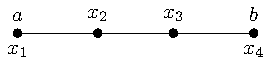
\includegraphics[width=0.35\textwidth]{fibonacci.pdf}
    \caption{Pontos do método de Fibonnaci}
   \label{fig:fib}
\end{figure}

Um fator de redução inicial $0.5<\alpha_1<0.7$ é usado para encontrar os primeiros valores de $x_2$ e $x_3$ dentro do intervalo enquadrante inicial $I_1 = [a \, b] \subset \mathbb{R}$. \\

Então, a função-objetivo é avaliada nesses dois pontos $x_2$ e $x_3$ e o intervalo é reduzido de acordo com a comparação dos valores de $f(x_2)= f_2$ e $f(x_3)=f_3$: se $f_2<f_3$, o novo intervalo é definido como $I_{k+1}=[x_1 \,x_3]$. Caso contrário, o intervalo seguinte passa a ser $I_{k+1}=[x_2 \,x_4]$. Finalmente, o fator de redução é recalculado de acordo com a equação \ref{eq:alpha} e o procedimento se repete até que o número de reduções desejado $n \in \mathbb{Z}$ seja atingido.

\begin{equation}
\alpha = \frac{L_{ini}-L_{fim}}{L_{fim}}
\label{eq:alpha}
\end{equation}

Novamente, o diagrama de fluxo do algoritmo implementado é apresentado na figura \ref{fig:fibonacci}.

\begin{figure}[h!]
\centering
\scalebox{0.85}{% This file was created by matlab2tikz.
%
%The latest updates can be retrieved from
%  http://www.mathworks.com/matlabcentral/fileexchange/22022-matlab2tikz-matlab2tikz
%where you can also make suggestions and rate matlab2tikz.
%
\definecolor{mycolor1}{rgb}{1.00000,1.00000,0.00000}%
%
\begin{tikzpicture}

\begin{axis}[%
width=4.521in,
height=3.566in,
at={(0.758in,0.481in)},
scale only axis,
separate axis lines,
every outer x axis line/.append style={black},
every x tick label/.append style={font=\color{black}},
xmin=-12.5,
xmax=5,
xlabel={$x$},
xmajorgrids,
every outer y axis line/.append style={black},
every y tick label/.append style={font=\color{black}},
ymin=-2000,
ymax=5000,
ylabel={$f(x)$},
ymajorgrids,
axis background/.style={fill=white},
title={M\'etodo de Fibonacci: $f(x) = x^4 + 10 x^3$}
]
\addplot [color=blue,solid,line width=2.0pt,forget plot]
  table[row sep=crcr]{%
-12.51	4914.11879001\\
-12.5	4882.8125\\
-12.49	4851.61871001\\
-12.48	4820.53718016\\
-12.47	4789.56767081\\
-12.46	4758.70994256\\
-12.45	4727.96375625\\
-12.44	4697.32887296\\
-12.43	4666.80505401\\
-12.42	4636.39206096\\
-12.41	4606.08965561\\
-12.4	4575.8976\\
-12.39	4545.81565641\\
-12.38	4515.84358736\\
-12.37	4485.98115561\\
-12.36	4456.22812416\\
-12.35	4426.58425625\\
-12.34	4397.04931536\\
-12.33	4367.62306521\\
-12.32	4338.30526976\\
-12.31	4309.09569321\\
-12.3	4279.9941\\
-12.29	4251.00025481\\
-12.28	4222.11392256\\
-12.27	4193.33486841\\
-12.26	4164.66285776\\
-12.25	4136.09765625\\
-12.24	4107.63902976\\
-12.23	4079.28674441\\
-12.22	4051.04056656\\
-12.21	4022.90026281\\
-12.2	3994.8656\\
-12.19	3966.93634521\\
-12.18	3939.11226576\\
-12.17	3911.39312921\\
-12.16	3883.77870336\\
-12.15	3856.26875625\\
-12.14	3828.86305616\\
-12.13	3801.56137161\\
-12.12	3774.36347136\\
-12.11	3747.26912441\\
-12.1	3720.2781\\
-12.09	3693.39016761\\
-12.08	3666.60509696\\
-12.07	3639.92265801\\
-12.06	3613.34262096\\
-12.05	3586.86475625\\
-12.04	3560.48883456\\
-12.03	3534.21462681\\
-12.02	3508.04190416\\
-12.01	3481.97043801\\
-12	3456\\
-11.99	3430.13036201\\
-11.98	3404.36129616\\
-11.97	3378.69257481\\
-11.96	3353.12397056\\
-11.95	3327.65525625\\
-11.94	3302.28620496\\
-11.93	3277.01659001\\
-11.92	3251.84618496\\
-11.91	3226.77476361\\
-11.9	3201.8021\\
-11.89	3176.92796841\\
-11.88	3152.15214336\\
-11.87	3127.47439961\\
-11.86	3102.89451216\\
-11.85	3078.41225625\\
-11.84	3054.02740736\\
-11.83	3029.73974121\\
-11.82	3005.54903376\\
-11.81	2981.45506121\\
-11.8	2957.45760000001\\
-11.79	2933.55642681\\
-11.78	2909.75131856\\
-11.77	2886.04205241\\
-11.76	2862.42840576\\
-11.75	2838.91015625\\
-11.74	2815.48708176\\
-11.73	2792.15896041\\
-11.72	2768.92557056\\
-11.71	2745.78669081\\
-11.7	2722.7421\\
-11.69	2699.79157721\\
-11.68	2676.93490176\\
-11.67	2654.17185321\\
-11.66	2631.50221136\\
-11.65	2608.92575625\\
-11.64	2586.44226816\\
-11.63	2564.05152761\\
-11.62	2541.75331536\\
-11.61	2519.54741241\\
-11.6	2497.4336\\
-11.59	2475.41165961\\
-11.58	2453.48137296\\
-11.57	2431.64252201\\
-11.56	2409.89488896\\
-11.55	2388.23825625\\
-11.54	2366.67240656\\
-11.53	2345.19712281\\
-11.52	2323.81218816\\
-11.51	2302.51738601\\
-11.5	2281.3125\\
-11.49	2260.19731401\\
-11.48	2239.17161216\\
-11.47	2218.23517881\\
-11.46	2197.38779856\\
-11.45	2176.62925625\\
-11.44	2155.95933696\\
-11.43	2135.37782601\\
-11.42	2114.88450896\\
-11.41	2094.47917161\\
-11.4	2074.1616\\
-11.39	2053.93158041\\
-11.38	2033.78889936\\
-11.37	2013.73334361\\
-11.36	1993.76470016\\
-11.35	1973.88275625\\
-11.34	1954.08729936\\
-11.33	1934.37811721\\
-11.32	1914.75499776\\
-11.31	1895.21772921\\
-11.3	1875.7661\\
-11.29	1856.39989881\\
-11.28	1837.11891456\\
-11.27	1817.92293641\\
-11.26	1798.81175376\\
-11.25	1779.78515625\\
-11.24	1760.84293376\\
-11.23	1741.98487641\\
-11.22	1723.21077456\\
-11.21	1704.52041881\\
-11.2	1685.9136\\
-11.19	1667.39010921\\
-11.18	1648.94973776\\
-11.17	1630.59227721\\
-11.16	1612.31751936\\
-11.15	1594.12525625\\
-11.14	1576.01528016\\
-11.13	1557.98738361\\
-11.12	1540.04135936\\
-11.11	1522.17700041\\
-11.1	1504.3941\\
-11.09	1486.69245161\\
-11.08	1469.07184896\\
-11.07	1451.53208601\\
-11.06	1434.07295696\\
-11.05	1416.69425625\\
-11.04	1399.39577856\\
-11.03	1382.17731881\\
-11.02	1365.03867216\\
-11.01	1347.97963401\\
-11	1331\\
-10.99	1314.09956601\\
-10.98	1297.27812816\\
-10.97	1280.53548281\\
-10.96	1263.87142656\\
-10.95	1247.28575625\\
-10.94	1230.77826896\\
-10.93	1214.34876201\\
-10.92	1197.99703296\\
-10.91	1181.72287961\\
-10.9	1165.5261\\
-10.89	1149.40649241\\
-10.88	1133.36385536\\
-10.87	1117.39798761\\
-10.86	1101.50868816\\
-10.85	1085.69575625\\
-10.84	1069.95899136\\
-10.83	1054.29819321\\
-10.82	1038.71316176\\
-10.81	1023.20369721\\
-10.8	1007.7696\\
-10.79	992.410670809999\\
-10.78	977.126710559998\\
-10.77	961.917520409999\\
-10.76	946.78290176\\
-10.75	931.72265625\\
-10.74	916.736585760002\\
-10.73	901.82449241\\
-10.72	886.986178559999\\
-10.71	872.221446809999\\
-10.7	857.5301\\
-10.69	842.911941209997\\
-10.68	828.366773759997\\
-10.67	813.89440121\\
-10.66	799.49462736\\
-10.65	785.167256250001\\
-10.64	770.912092159999\\
-10.63	756.728939609999\\
-10.62	742.61760336\\
-10.61	728.577888409998\\
-10.6	714.6096\\
-10.59	700.71254361\\
-10.58	686.88652496\\
-10.57	673.13135001\\
-10.56	659.446824960001\\
-10.55	645.83275625\\
-10.54	632.28895056\\
-10.53	618.81521481\\
-10.52	605.411356160001\\
-10.51	592.07718201\\
-10.5	578.8125\\
-10.49	565.617118010001\\
-10.48	552.49084416\\
-10.47	539.433486809998\\
-10.46	526.444854560001\\
-10.45	513.524756249999\\
-10.44	500.67300096\\
-10.43	487.889398009998\\
-10.42	475.173756960001\\
-10.41	462.52588761\\
-10.4	449.945600000003\\
-10.39	437.432704410001\\
-10.38	424.987011360001\\
-10.37	412.608331609998\\
-10.36	400.29647616\\
-10.35	388.051256249999\\
-10.34	375.872483359999\\
-10.33	363.759969210001\\
-10.32	351.71352576\\
-10.31	339.732965209998\\
-10.3	327.818099999999\\
-10.29	315.968742809999\\
-10.28	304.18470656\\
-10.27	292.465804409998\\
-10.26	280.811849759999\\
-10.25	269.22265625\\
-10.24	257.698037759998\\
-10.23	246.23780841\\
-10.22	234.841782559999\\
-10.21	223.50977481\\
-10.2	212.241599999999\\
-10.19	201.03707321\\
-10.18	189.896009760001\\
-10.17	178.81822521\\
-10.16	167.803535359999\\
-10.15	156.851756249998\\
-10.14	145.962704160002\\
-10.13	135.136195609999\\
-10.12	124.372047359999\\
-10.11	113.670076410001\\
-10.1	103.0301\\
-10.09	92.4519356099991\\
-10.08	81.9354009600011\\
-10.07	71.4803140099993\\
-10.06	61.0864929599975\\
-10.05	50.753756250002\\
-10.04	40.4819225599986\\
-10.03	30.2708108099978\\
-10.02	20.1202401600003\\
-10.01	10.0300300100007\\
-10	0\\
-9.99	-9.9700299899996\\
-9.98	-19.8802398400003\\
-9.97	-29.7308091900013\\
-9.96	-39.5219174400008\\
-9.95	-49.2537437500014\\
-9.94	-58.9264670400007\\
-9.93	-68.5402659899992\\
-9.92	-78.0953190399996\\
-9.91	-87.5918043900001\\
-9.9	-97.0298999999995\\
-9.89	-106.409783589999\\
-9.88	-115.731632640001\\
-9.87	-124.995624390001\\
-9.86	-134.201935840001\\
-9.85	-143.350743750001\\
-9.84	-152.442224639999\\
-9.83	-161.476554789999\\
-9.82	-170.453910239999\\
-9.81	-179.374466790003\\
-9.8	-188.238399999998\\
-9.79	-197.04588519\\
-9.78	-205.797097440001\\
-9.77	-214.492211590001\\
-9.76	-223.13140224\\
-9.75	-231.71484375\\
-9.74	-240.24271024\\
-9.73	-248.715175589999\\
-9.72	-257.13241344\\
-9.71	-265.494597190002\\
-9.7	-273.8019\\
-9.69	-282.05449479\\
-9.68	-290.25255424\\
-9.67	-298.39625079\\
-9.66	-306.485756640001\\
-9.65	-314.521243749999\\
-9.64	-322.502883839999\\
-9.63	-330.43084839\\
-9.62	-338.30530864\\
-9.61	-346.12643559\\
-9.6	-353.894399999999\\
-9.59	-361.609372390001\\
-9.58	-369.271523040001\\
-9.57	-376.881021990001\\
-9.56	-384.438039040002\\
-9.55	-391.942743749998\\
-9.54	-399.395305440001\\
-9.53	-406.795893190001\\
-9.52	-414.14467584\\
-9.51	-421.44182199\\
-9.5	-428.6875\\
-9.49	-435.881877990001\\
-9.48	-443.025123840001\\
-9.47	-450.117405190001\\
-9.46	-457.15888944\\
-9.45	-464.149743750001\\
-9.44	-471.090135040001\\
-9.43	-477.980229989999\\
-9.42	-484.820195040001\\
-9.41	-491.61019639\\
-9.4	-498.350399999999\\
-9.39	-505.040971590001\\
-9.38	-511.682076640001\\
-9.37	-518.273880390001\\
-9.36	-524.816547840001\\
-9.35	-531.310243750001\\
-9.34	-537.75513264\\
-9.33	-544.151378789999\\
-9.32	-550.49914624\\
-9.31	-556.798598790001\\
-9.3	-563.049899999999\\
-9.29	-569.25321319\\
-9.28	-575.40870144\\
-9.27	-581.51652759\\
-9.26	-587.57685424\\
-9.25	-593.58984375\\
-9.24	-599.55565824\\
-9.23	-605.47445959\\
-9.22	-611.346409440001\\
-9.21	-617.171669190001\\
-9.2	-622.950400000002\\
-9.19	-628.68276279\\
-9.18	-634.36891824\\
-9.17	-640.00902679\\
-9.16	-645.603248639999\\
-9.15	-651.151743750001\\
-9.14	-656.65467184\\
-9.13	-662.112192390001\\
-9.12	-667.52446464\\
-9.11	-672.89164759\\
-9.1	-678.213900000001\\
-9.09	-683.491380390001\\
-9.08	-688.724247039999\\
-9.07	-693.91265799\\
-9.06	-699.05677104\\
-9.05	-704.15674375\\
-9.04	-709.212733439999\\
-9.03	-714.224897190001\\
-9.02	-719.19339184\\
-9.01	-724.11837399\\
-9	-729\\
-8.99	-733.83842599\\
-8.98	-738.63380784\\
-8.97	-743.386301189999\\
-8.96	-748.096061440001\\
-8.95	-752.76324375\\
-8.94	-757.38800304\\
-8.93	-761.97049399\\
-8.92	-766.51087104\\
-8.91	-771.009288390001\\
-8.9	-775.465899999999\\
-8.89	-779.88085959\\
-8.88	-784.254320640001\\
-8.87	-788.58643639\\
-8.86	-792.87735984\\
-8.85	-797.12724375\\
-8.84	-801.33624064\\
-8.83	-805.50450279\\
-8.82	-809.63218224\\
-8.81	-813.71943079\\
-8.8	-817.7664\\
-8.79	-821.77324119\\
-8.78	-825.74010544\\
-8.77	-829.66714359\\
-8.76	-833.554506240001\\
-8.75	-837.40234375\\
-8.74	-841.21080624\\
-8.73	-844.980043590001\\
-8.72	-848.71020544\\
-8.71	-852.401441190001\\
-8.7	-856.0539\\
-8.69	-859.66773079\\
-8.68	-863.243082239999\\
-8.67	-866.78010279\\
-8.66	-870.27894064\\
-8.65	-873.739743749999\\
-8.64	-877.162659840001\\
-8.63	-880.547836389999\\
-8.62	-883.895420640001\\
-8.61	-887.20555959\\
-8.6	-890.4784\\
-8.59	-893.714088389999\\
-8.58	-896.912771040001\\
-8.57	-900.074593990001\\
-8.56	-903.19970304\\
-8.55	-906.28824375\\
-8.54	-909.340361439999\\
-8.53	-912.356201190001\\
-8.52	-915.33590784\\
-8.51	-918.27962599\\
-8.5	-921.1875\\
-8.49	-924.059673990001\\
-8.48	-926.89629184\\
-8.47	-929.69749719\\
-8.46	-932.46343344\\
-8.45	-935.194243750001\\
-8.44	-937.890071039999\\
-8.43	-940.55105799\\
-8.42	-943.17734704\\
-8.41	-945.76908039\\
-8.4	-948.326400000001\\
-8.39	-950.84944759\\
-8.38	-953.33836464\\
-8.37	-955.793292390001\\
-8.36	-958.21437184\\
-8.35	-960.60174375\\
-8.34	-962.95554864\\
-8.33	-965.27592679\\
-8.32	-967.56301824\\
-8.31	-969.816962790001\\
-8.3	-972.0379\\
-8.29	-974.22596919\\
-8.28	-976.38130944\\
-8.27	-978.50405959\\
-8.26	-980.59435824\\
-8.25	-982.65234375\\
-8.24	-984.67815424\\
-8.23	-986.67192759\\
-8.22	-988.63380144\\
-8.21	-990.56391319\\
-8.2	-992.4624\\
-8.19	-994.32939879\\
-8.18	-996.165046239999\\
-8.17	-997.969478790001\\
-8.16	-999.742832640001\\
-8.15	-1001.48524375\\
-8.14	-1003.19684784\\
-8.13	-1004.87778039\\
-8.12	-1006.52817664\\
-8.11	-1008.14817159\\
-8.1	-1009.7379\\
-8.09	-1011.29749639\\
-8.08	-1012.82709504\\
-8.07	-1014.32682999\\
-8.06	-1015.79683504\\
-8.05	-1017.23724375\\
-8.04	-1018.64818944\\
-8.03	-1020.02980519\\
-8.02	-1021.38222384\\
-8.01	-1022.70557799\\
-8	-1024\\
-7.99	-1025.26562199\\
-7.98	-1026.50257584\\
-7.97	-1027.71099319\\
-7.96	-1028.89100544\\
-7.95	-1030.04274375\\
-7.94	-1031.16633904\\
-7.93	-1032.26192199\\
-7.92	-1033.32962304\\
-7.91	-1034.36957239\\
-7.9	-1035.3819\\
-7.89	-1036.36673559\\
-7.88	-1037.32420864\\
-7.87	-1038.25444839\\
-7.86	-1039.15758384\\
-7.85	-1040.03374375\\
-7.84	-1040.88305664\\
-7.83	-1041.70565079\\
-7.82	-1042.50165424\\
-7.81	-1043.27119479\\
-7.8	-1044.0144\\
-7.79	-1044.73139719\\
-7.78	-1045.42231344\\
-7.77	-1046.08727559\\
-7.76	-1046.72641024\\
-7.75	-1047.33984375\\
-7.74	-1047.92770224\\
-7.73	-1048.49011159\\
-7.72	-1049.02719744\\
-7.71	-1049.53908519\\
-7.7	-1050.0259\\
-7.69	-1050.48776679\\
-7.68	-1050.92481024\\
-7.67	-1051.33715479\\
-7.66	-1051.72492464\\
-7.65	-1052.08824375\\
-7.64	-1052.42723584\\
-7.63	-1052.74202439\\
-7.62	-1053.03273264\\
-7.61	-1053.29948359\\
-7.6	-1053.5424\\
-7.59	-1053.76160439\\
-7.58	-1053.95721904\\
-7.57	-1054.12936599\\
-7.56	-1054.27816704\\
-7.55	-1054.40374375\\
-7.54	-1054.50621744\\
-7.53	-1054.58570919\\
-7.52	-1054.64233984\\
-7.51	-1054.67622999\\
-7.5	-1054.6875\\
-7.49	-1054.67626999\\
-7.48	-1054.64265984\\
-7.47	-1054.58678919\\
-7.46	-1054.50877744\\
-7.45	-1054.40874375\\
-7.44	-1054.28680704\\
-7.43	-1054.14308599\\
-7.42	-1053.97769904\\
-7.41	-1053.79076439\\
-7.4	-1053.5824\\
-7.39	-1053.35272359\\
-7.38	-1053.10185264\\
-7.37	-1052.82990439\\
-7.36	-1052.53699584\\
-7.35	-1052.22324375\\
-7.34	-1051.88876464\\
-7.33	-1051.53367479\\
-7.32	-1051.15809024\\
-7.31	-1050.76212679\\
-7.3	-1050.3459\\
-7.29	-1049.90952519\\
-7.28	-1049.45311744\\
-7.27	-1048.97679159\\
-7.26	-1048.48066224\\
-7.25	-1047.96484375\\
-7.24	-1047.42945024\\
-7.23	-1046.87459559\\
-7.22	-1046.30039344\\
-7.21	-1045.70695719\\
-7.2	-1045.0944\\
-7.19	-1044.46283479\\
-7.18	-1043.81237424\\
-7.17	-1043.14313079\\
-7.16	-1042.45521664\\
-7.15	-1041.74874375\\
-7.14	-1041.02382384\\
-7.13	-1040.28056839\\
-7.12	-1039.51908864\\
-7.11	-1038.73949559\\
-7.1	-1037.9419\\
-7.09	-1037.12641239\\
-7.08	-1036.29314304\\
-7.07	-1035.44220199\\
-7.06	-1034.57369904\\
-7.05	-1033.68774375\\
-7.04	-1032.78444544\\
-7.03	-1031.86391319\\
-7.02	-1030.92625584\\
-7.01	-1029.97158199\\
-7	-1029\\
-6.99	-1028.01161799\\
-6.98	-1027.00654384\\
-6.97	-1025.98488519\\
-6.96	-1024.94674944\\
-6.95	-1023.89224375\\
-6.94	-1022.82147504\\
-6.93	-1021.73454999\\
-6.92	-1020.63157504\\
-6.91	-1019.51265639\\
-6.9	-1018.3779\\
-6.89	-1017.22741159\\
-6.88	-1016.06129664\\
-6.87	-1014.87966039\\
-6.86	-1013.68260784\\
-6.85	-1012.47024375\\
-6.84	-1011.24267264\\
-6.83	-1009.99999879\\
-6.82	-1008.74232624\\
-6.81	-1007.46975879\\
-6.8	-1006.1824\\
-6.79	-1004.88035319\\
-6.78	-1003.56372144\\
-6.77	-1002.23260759\\
-6.76	-1000.88711424\\
-6.75	-999.52734375\\
-6.74	-998.15339824\\
-6.73	-996.76537959\\
-6.72	-995.36338944\\
-6.71	-993.94752919\\
-6.7	-992.5179\\
-6.69	-991.07460279\\
-6.68	-989.61773824\\
-6.67	-988.14740679\\
-6.66	-986.66370864\\
-6.65	-985.16674375\\
-6.64	-983.65661184\\
-6.63	-982.13341239\\
-6.62	-980.59724464\\
-6.61	-979.04820759\\
-6.6	-977.4864\\
-6.59	-975.91192039\\
-6.58	-974.32486704\\
-6.57	-972.72533799\\
-6.56	-971.11343104\\
-6.55	-969.48924375\\
-6.54	-967.85287344\\
-6.53	-966.20441719\\
-6.52	-964.54397184\\
-6.51	-962.87163399\\
-6.5	-961.1875\\
-6.49	-959.49166599\\
-6.48	-957.78422784\\
-6.47	-956.06528119\\
-6.46	-954.33492144\\
-6.45	-952.59324375\\
-6.44	-950.84034304\\
-6.43	-949.07631399\\
-6.42	-947.30125104\\
-6.41	-945.51524839\\
-6.4	-943.7184\\
-6.39	-941.91079959\\
-6.38	-940.09254064\\
-6.37	-938.26371639\\
-6.36	-936.42441984\\
-6.35	-934.57474375\\
-6.34	-932.71478064\\
-6.33	-930.84462279\\
-6.32	-928.96436224\\
-6.31	-927.07409079\\
-6.3	-925.1739\\
-6.29	-923.26388119\\
-6.28	-921.34412544\\
-6.27	-919.41472359\\
-6.26	-917.47576624\\
-6.25	-915.52734375\\
-6.24	-913.56954624\\
-6.23	-911.60246359\\
-6.22	-909.62618544\\
-6.21	-907.64080119\\
-6.2	-905.6464\\
-6.19	-903.64307079\\
-6.18	-901.63090224\\
-6.17	-899.60998279\\
-6.16	-897.58040064\\
-6.15	-895.54224375\\
-6.14	-893.49559984\\
-6.13	-891.44055639\\
-6.12	-889.37720064\\
-6.11	-887.30561959\\
-6.1	-885.2259\\
-6.09	-883.13812839\\
-6.08	-881.04239104\\
-6.07	-878.93877399\\
-6.06	-876.82736304\\
-6.05	-874.70824375\\
-6.04	-872.58150144\\
-6.03	-870.44722119\\
-6.02	-868.30548784\\
-6.01	-866.15638599\\
-6	-864\\
-5.99	-861.83641399\\
-5.98	-859.66571184\\
-5.97	-857.48797719\\
-5.96	-855.30329344\\
-5.95	-853.11174375\\
-5.94	-850.91341104\\
-5.93	-848.70837799\\
-5.92	-846.49672704\\
-5.91	-844.27854039\\
-5.9	-842.0539\\
-5.89	-839.82288759\\
-5.88	-837.58558464\\
-5.87	-835.34207239\\
-5.86	-833.09243184\\
-5.85	-830.83674375\\
-5.84	-828.57508864\\
-5.83	-826.30754679\\
-5.82	-824.03419824\\
-5.81	-821.75512279\\
-5.8	-819.4704\\
-5.79	-817.18010919\\
-5.78	-814.88432944\\
-5.77	-812.58313959\\
-5.76	-810.27661824\\
-5.75	-807.96484375\\
-5.74	-805.64789424\\
-5.73	-803.32584759\\
-5.72	-800.99878144\\
-5.71	-798.66677319\\
-5.7	-796.3299\\
-5.69	-793.98823879\\
-5.68	-791.64186624\\
-5.67	-789.29085879\\
-5.66	-786.93529264\\
-5.65	-784.57524375\\
-5.64	-782.21078784\\
-5.63	-779.84200039\\
-5.62	-777.46895664\\
-5.61	-775.09173159\\
-5.6	-772.7104\\
-5.59	-770.32503639\\
-5.58	-767.93571504\\
-5.57	-765.54250999\\
-5.56	-763.14549504\\
-5.55	-760.74474375\\
-5.54	-758.34032944\\
-5.53	-755.93232519\\
-5.52	-753.52080384\\
-5.51	-751.10583799\\
-5.5	-748.6875\\
-5.49	-746.26586199\\
-5.48	-743.84099584\\
-5.47	-741.41297319\\
-5.46	-738.98186544\\
-5.45	-736.54774375\\
-5.44	-734.11067904\\
-5.43	-731.67074199\\
-5.42	-729.22800304\\
-5.41	-726.78253239\\
-5.4	-724.3344\\
-5.39	-721.88367559\\
-5.38	-719.43042864\\
-5.37	-716.97472839\\
-5.36	-714.51664384\\
-5.35	-712.05624375\\
-5.34	-709.59359664\\
-5.33	-707.12877079\\
-5.32	-704.66183424\\
-5.31	-702.19285479\\
-5.3	-699.7219\\
-5.29	-697.24903719\\
-5.28	-694.77433344\\
-5.27	-692.29785559\\
-5.26	-689.81967024\\
-5.25	-687.33984375\\
-5.24	-684.85844224\\
-5.23	-682.37553159\\
-5.22	-679.89117744\\
-5.21	-677.40544519\\
-5.2	-674.9184\\
-5.19	-672.43010679\\
-5.18	-669.94063024\\
-5.17	-667.45003479\\
-5.16	-664.95838464\\
-5.15	-662.46574375\\
-5.14	-659.97217584\\
-5.13	-657.47774439\\
-5.12	-654.98251264\\
-5.11	-652.48654359\\
-5.1	-649.9899\\
-5.09	-647.49264439\\
-5.08	-644.99483904\\
-5.07	-642.49654599\\
-5.06	-639.99782704\\
-5.05	-637.49874375\\
-5.04	-634.99935744\\
-5.03	-632.49972919\\
-5.02	-629.99991984\\
-5.01	-627.49998999\\
-5	-625\\
-4.99	-622.50000999\\
-4.98	-620.00007984\\
-4.97	-617.50026919\\
-4.96	-615.00063744\\
-4.95	-612.50124375\\
-4.94	-610.00214704\\
-4.93	-607.50340599\\
-4.92	-605.00507904\\
-4.91	-602.50722439\\
-4.9	-600.0099\\
-4.89	-597.51316359\\
-4.88	-595.01707264\\
-4.87	-592.52168439\\
-4.86	-590.02705584\\
-4.85	-587.53324375\\
-4.84	-585.04030464\\
-4.83	-582.54829479\\
-4.82	-580.05727024\\
-4.81	-577.56728679\\
-4.8	-575.0784\\
-4.79	-572.59066519\\
-4.78	-570.10413744\\
-4.77	-567.61887159\\
-4.76	-565.13492224\\
-4.75	-562.65234375\\
-4.74	-560.17119024\\
-4.73	-557.69151559\\
-4.72	-555.21337344\\
-4.71	-552.73681719\\
-4.7	-550.2619\\
-4.69	-547.78867479\\
-4.68	-545.31719424\\
-4.67	-542.84751079\\
-4.66	-540.37967664\\
-4.65	-537.91374375\\
-4.64	-535.44976384\\
-4.63	-532.98778839\\
-4.62	-530.52786864\\
-4.61	-528.07005559\\
-4.6	-525.6144\\
-4.59	-523.16095239\\
-4.58	-520.70976304\\
-4.57	-518.26088199\\
-4.56	-515.81435904\\
-4.55	-513.37024375\\
-4.54	-510.92858544\\
-4.53	-508.48943319\\
-4.52	-506.05283584\\
-4.51	-503.61884199\\
-4.5	-501.1875\\
-4.49	-498.75885799\\
-4.48	-496.33296384\\
-4.47	-493.90986519\\
-4.46	-491.48960944\\
-4.45	-489.07224375\\
-4.44	-486.65781504\\
-4.43	-484.24636999\\
-4.42	-481.83795504\\
-4.41	-479.43261639\\
-4.4	-477.0304\\
-4.39	-474.63135159\\
-4.38	-472.23551664\\
-4.37	-469.84294039\\
-4.36	-467.45366784\\
-4.35	-465.06774375\\
-4.34	-462.68521264\\
-4.33	-460.30611879\\
-4.32	-457.93050624\\
-4.31	-455.55841879\\
-4.3	-453.1899\\
-4.29	-450.82499319\\
-4.28	-448.46374144\\
-4.27	-446.10618759\\
-4.26	-443.75237424\\
-4.25	-441.40234375\\
-4.24	-439.05613824\\
-4.23	-436.71379959\\
-4.22	-434.37536944\\
-4.21	-432.04088919\\
-4.2	-429.7104\\
-4.19	-427.38394279\\
-4.18	-425.06155824\\
-4.17	-422.74328679\\
-4.16	-420.42916864\\
-4.15	-418.11924375\\
-4.14	-415.81355184\\
-4.13	-413.51213239\\
-4.12	-411.21502464\\
-4.11	-408.92226759\\
-4.1	-406.6339\\
-4.09	-404.34996039\\
-4.08	-402.07048704\\
-4.07	-399.79551799\\
-4.06	-397.52509104\\
-4.05	-395.25924375\\
-4.04	-392.99801344\\
-4.03	-390.74143719\\
-4.02	-388.48955184\\
-4.01	-386.24239399\\
-4	-384\\
-3.99	-381.76240599\\
-3.98	-379.52964784\\
-3.97	-377.30176119\\
-3.96	-375.07878144\\
-3.95	-372.86074375\\
-3.94	-370.64768304\\
-3.93	-368.43963399\\
-3.92	-366.23663104\\
-3.91	-364.03870839\\
-3.9	-361.8459\\
-3.89	-359.65823959\\
-3.88	-357.47576064\\
-3.87	-355.29849639\\
-3.86	-353.12647984\\
-3.85	-350.95974375\\
-3.84	-348.79832064\\
-3.83	-346.64224279\\
-3.82	-344.49154224\\
-3.81	-342.34625079\\
-3.8	-340.2064\\
-3.79	-338.07202119\\
-3.78	-335.94314544\\
-3.77	-333.81980359\\
-3.76	-331.70202624\\
-3.75	-329.58984375\\
-3.74	-327.48328624\\
-3.73	-325.38238359\\
-3.72	-323.28716544\\
-3.71	-321.19766119\\
-3.7	-319.1139\\
-3.69	-317.03591079\\
-3.68	-314.96372224\\
-3.67	-312.89736279\\
-3.66	-310.83686064\\
-3.65	-308.78224375\\
-3.64	-306.73353984\\
-3.63	-304.69077639\\
-3.62	-302.65398064\\
-3.61	-300.62317959\\
-3.6	-298.5984\\
-3.59	-296.57966839\\
-3.58	-294.56701104\\
-3.57	-292.56045399\\
-3.56	-290.56002304\\
-3.55	-288.56574375\\
-3.54	-286.57764144\\
-3.53	-284.59574119\\
-3.52	-282.62006784\\
-3.51	-280.65064599\\
-3.5	-278.6875\\
-3.49	-276.73065399\\
-3.48	-274.78013184\\
-3.47	-272.83595719\\
-3.46	-270.89815344\\
-3.45	-268.96674375\\
-3.44	-267.04175104\\
-3.43	-265.12319799\\
-3.42	-263.21110704\\
-3.41	-261.30550039\\
-3.4	-259.4064\\
-3.39	-257.51382759\\
-3.38	-255.62780464\\
-3.37	-253.74835239\\
-3.36	-251.87549184\\
-3.35	-250.00924375\\
-3.34	-248.14962864\\
-3.33	-246.29666679\\
-3.32	-244.45037824\\
-3.31	-242.61078279\\
-3.3	-240.7779\\
-3.29	-238.95174919\\
-3.28	-237.13234944\\
-3.27	-235.31971959\\
-3.26	-233.51387824\\
-3.25	-231.71484375\\
-3.24	-229.92263424\\
-3.23	-228.13726759\\
-3.22	-226.35876144\\
-3.21	-224.58713319\\
-3.2	-222.8224\\
-3.19	-221.06457879\\
-3.18	-219.31368624\\
-3.17	-217.56973879\\
-3.16	-215.83275264\\
-3.15	-214.10274375\\
-3.14	-212.37972784\\
-3.13	-210.66372039\\
-3.12	-208.95473664\\
-3.11	-207.25279159\\
-3.1	-205.5579\\
-3.09	-203.87007639\\
-3.08	-202.18933504\\
-3.07	-200.51568999\\
-3.06	-198.84915504\\
-3.05	-197.18974375\\
-3.04	-195.53746944\\
-3.03	-193.89234519\\
-3.02	-192.25438384\\
-3.01	-190.62359799\\
-3	-189\\
-2.99	-187.38360199\\
-2.98	-185.77441584\\
-2.97	-184.17245319\\
-2.96	-182.57772544\\
-2.95	-180.99024375\\
-2.94	-179.41001904\\
-2.93	-177.83706199\\
-2.92	-176.27138304\\
-2.91	-174.71299239\\
-2.9	-173.1619\\
-2.89	-171.61811559\\
-2.88	-170.08164864\\
-2.87	-168.55250839\\
-2.86	-167.03070384\\
-2.85	-165.51624375\\
-2.84	-164.00913664\\
-2.83	-162.50939079\\
-2.82	-161.01701424\\
-2.81	-159.53201479\\
-2.8	-158.0544\\
-2.79	-156.58417719\\
-2.78	-155.12135344\\
-2.77	-153.66593559\\
-2.76	-152.21793024\\
-2.75	-150.77734375\\
-2.74	-149.34418224\\
-2.73	-147.91845159\\
-2.72	-146.50015744\\
-2.71	-145.08930519\\
-2.7	-143.6859\\
-2.69	-142.28994679\\
-2.68	-140.90145024\\
-2.67	-139.52041479\\
-2.66	-138.14684464\\
-2.65	-136.78074375\\
-2.64	-135.42211584\\
-2.63	-134.07096439\\
-2.62	-132.72729264\\
-2.61	-131.39110359\\
-2.6	-130.0624\\
-2.59	-128.74118439\\
-2.58	-127.42745904\\
-2.57	-126.12122599\\
-2.56	-124.82248704\\
-2.55	-123.53124375\\
-2.54	-122.24749744\\
-2.53	-120.97124919\\
-2.52	-119.70249984\\
-2.51	-118.44124999\\
-2.5	-117.1875\\
-2.49	-115.94124999\\
-2.48	-114.70249984\\
-2.47	-113.47124919\\
-2.46	-112.24749744\\
-2.45	-111.03124375\\
-2.44	-109.82248704\\
-2.43	-108.62122599\\
-2.42	-107.42745904\\
-2.41	-106.24118439\\
-2.4	-105.0624\\
-2.39	-103.89110359\\
-2.38	-102.72729264\\
-2.37	-101.57096439\\
-2.36	-100.42211584\\
-2.35	-99.2807437500001\\
-2.34	-98.1468446400001\\
-2.33	-97.02041479\\
-2.32	-95.90145024\\
-2.31	-94.7899467900001\\
-2.3	-93.6859000000001\\
-2.29	-92.58930519\\
-2.28	-91.50015744\\
-2.27	-90.41845159\\
-2.26	-89.3441822400001\\
-2.25	-88.27734375\\
-2.24	-87.21793024\\
-2.23	-86.16593559\\
-2.22	-85.1213534400001\\
-2.21	-84.08417719\\
-2.2	-83.0544\\
-2.19	-82.03201479\\
-2.18	-81.0170142400001\\
-2.17	-80.00939079\\
-2.16	-79.00913664\\
-2.15	-78.01624375\\
-2.14	-77.0307038400001\\
-2.13	-76.0525083900001\\
-2.12	-75.08164864\\
-2.11	-74.11811559\\
-2.1	-73.1619000000001\\
-2.09	-72.2129923900001\\
-2.08	-71.27138304\\
-2.07	-70.33706199\\
-2.06	-69.4100190400001\\
-2.05	-68.4902437500001\\
-2.04	-67.57772544\\
-2.03	-66.67245319\\
-2.02	-65.77441584\\
-2.01	-64.8836019900001\\
-2	-64\\
-1.99	-63.12359799\\
-1.98	-62.25438384\\
-1.97	-61.3923451900001\\
-1.96	-60.53746944\\
-1.95	-59.68974375\\
-1.94	-58.84915504\\
-1.93	-58.01568999\\
-1.92	-57.18933504\\
-1.91	-56.37007639\\
-1.9	-55.5579\\
-1.89	-54.75279159\\
-1.88	-53.9547366400001\\
-1.87	-53.16372039\\
-1.86	-52.37972784\\
-1.85	-51.60274375\\
-1.84	-50.8327526400001\\
-1.83	-50.06973879\\
-1.82	-49.31368624\\
-1.81	-48.56457879\\
-1.8	-47.8224000000001\\
-1.79	-47.08713319\\
-1.78	-46.35876144\\
-1.77	-45.63726759\\
-1.76	-44.92263424\\
-1.75	-44.21484375\\
-1.74	-43.51387824\\
-1.73	-42.81971959\\
-1.72	-42.13234944\\
-1.71	-41.45174919\\
-1.7	-40.7779\\
-1.69	-40.11078279\\
-1.68	-39.45037824\\
-1.67	-38.79666679\\
-1.66	-38.14962864\\
-1.65	-37.50924375\\
-1.64	-36.87549184\\
-1.63	-36.24835239\\
-1.62	-35.62780464\\
-1.61	-35.01382759\\
-1.6	-34.4064\\
-1.59	-33.80550039\\
-1.58	-33.21110704\\
-1.57	-32.62319799\\
-1.56	-32.04175104\\
-1.55	-31.46674375\\
-1.54	-30.89815344\\
-1.53	-30.33595719\\
-1.52	-29.78013184\\
-1.51	-29.23065399\\
-1.5	-28.6875\\
-1.49	-28.15064599\\
-1.48	-27.62006784\\
-1.47	-27.09574119\\
-1.46	-26.57764144\\
-1.45	-26.06574375\\
-1.44	-25.56002304\\
-1.43	-25.06045399\\
-1.42	-24.56701104\\
-1.41	-24.07966839\\
-1.4	-23.5984\\
-1.39	-23.12317959\\
-1.38	-22.65398064\\
-1.37	-22.19077639\\
-1.36	-21.73353984\\
-1.35	-21.28224375\\
-1.34	-20.83686064\\
-1.33	-20.39736279\\
-1.32	-19.96372224\\
-1.31	-19.53591079\\
-1.3	-19.1139\\
-1.29	-18.69766119\\
-1.28	-18.28716544\\
-1.27	-17.88238359\\
-1.26	-17.48328624\\
-1.25	-17.08984375\\
-1.24	-16.70202624\\
-1.23	-16.31980359\\
-1.22	-15.94314544\\
-1.21	-15.57202119\\
-1.2	-15.2064\\
-1.19	-14.84625079\\
-1.18	-14.49154224\\
-1.17	-14.14224279\\
-1.16	-13.79832064\\
-1.15	-13.45974375\\
-1.14	-13.12647984\\
-1.13	-12.79849639\\
-1.12	-12.47576064\\
-1.11	-12.15823959\\
-1.1	-11.8459\\
-1.09	-11.53870839\\
-1.08	-11.23663104\\
-1.07	-10.93963399\\
-1.06	-10.64768304\\
-1.05	-10.36074375\\
-1.04	-10.07878144\\
-1.03	-9.80176119000001\\
-1.02	-9.52964784000001\\
-1.01	-9.26240599000002\\
-1	-9\\
-0.99	-8.74239399\\
-0.98	-8.48955184000001\\
-0.970000000000001	-8.24143719000002\\
-0.96	-7.99801344\\
-0.95	-7.75924375\\
-0.94	-7.52509104000001\\
-0.930000000000001	-7.29551799000001\\
-0.92	-7.07048704\\
-0.91	-6.84996039\\
-0.9	-6.63390000000001\\
-0.890000000000001	-6.42226759000001\\
-0.88	-6.21502464\\
-0.87	-6.01213239\\
-0.86	-5.81355184000001\\
-0.850000000000001	-5.61924375000001\\
-0.840000000000001	-5.42916864000001\\
-0.83	-5.24328679\\
-0.82	-5.06155824\\
-0.810000000000001	-4.88394279000001\\
-0.800000000000001	-4.71040000000001\\
-0.79	-4.54088919\\
-0.78	-4.37536944\\
-0.77	-4.21379959000001\\
-0.760000000000001	-4.05613824000001\\
-0.75	-3.90234375\\
-0.74	-3.75237424\\
-0.73	-3.60618759000001\\
-0.720000000000001	-3.46374144000001\\
-0.71	-3.32499319\\
-0.7	-3.1899\\
-0.69	-3.05841879000001\\
-0.680000000000001	-2.93050624000001\\
-0.67	-2.80611879\\
-0.66	-2.68521264\\
-0.65	-2.56774375\\
-0.640000000000001	-2.45366784000001\\
-0.63	-2.34294039\\
-0.62	-2.23551664\\
-0.61	-2.13135159\\
-0.600000000000001	-2.03040000000001\\
-0.590000000000001	-1.93261639000001\\
-0.58	-1.83795504\\
-0.57	-1.74636999\\
-0.560000000000001	-1.65781504\\
-0.550000000000001	-1.57224375000001\\
-0.54	-1.48960944\\
-0.53	-1.40986519\\
-0.52	-1.33296384\\
-0.510000000000001	-1.25885799\\
-0.5	-1.1875\\
-0.49	-1.11884199\\
-0.48	-1.05283584\\
-0.470000000000001	-0.989433190000004\\
-0.46	-0.92858544\\
-0.45	-0.870243750000001\\
-0.44	-0.814359040000002\\
-0.430000000000001	-0.760881990000003\\
-0.42	-0.70976304\\
-0.41	-0.660952390000001\\
-0.4	-0.614400000000002\\
-0.390000000000001	-0.570055590000002\\
-0.38	-0.52786864\\
-0.37	-0.48778839\\
-0.36	-0.449763840000001\\
-0.350000000000001	-0.413743750000002\\
-0.340000000000001	-0.379676640000002\\
-0.33	-0.34751079\\
-0.32	-0.317194240000001\\
-0.310000000000001	-0.288674790000001\\
-0.300000000000001	-0.261900000000002\\
-0.29	-0.23681719\\
-0.28	-0.213373440000001\\
-0.27	-0.191515590000001\\
-0.260000000000001	-0.171190240000001\\
-0.25	-0.15234375\\
-0.24	-0.13492224\\
-0.23	-0.118871590000001\\
-0.220000000000001	-0.104137440000001\\
-0.21	-0.0906651899999999\\
-0.2	-0.0784000000000002\\
-0.19	-0.0672867900000004\\
-0.180000000000001	-0.0572702400000006\\
-0.17	-0.0482947899999999\\
-0.16	-0.0403046400000001\\
-0.15	-0.0332437500000002\\
-0.140000000000001	-0.0270558400000003\\
-0.13	-0.0216843899999999\\
-0.12	-0.01707264\\
-0.11	-0.0131635900000001\\
-0.100000000000001	-0.00990000000000016\\
-0.0900000000000007	-0.00722439000000018\\
-0.0800000000000001	-0.00507904000000001\\
-0.0700000000000003	-0.00340599000000004\\
-0.0600000000000005	-0.00214704000000005\\
-0.0500000000000007	-0.00124375000000005\\
-0.04	-0.000637440000000002\\
-0.0300000000000002	-0.000269190000000007\\
-0.0200000000000005	-7.98400000000055e-05\\
-0.0100000000000007	-9.99000000000202e-06\\
0	0\\
0.00999999999999979	1.00099999999994e-05\\
0.0199999999999996	8.01599999999949e-05\\
0.0299999999999994	0.000270809999999983\\
0.04	0.000642560000000002\\
0.0499999999999998	0.00125624999999999\\
0.0599999999999996	0.00217295999999996\\
0.0699999999999994	0.00345400999999991\\
0.0800000000000001	0.00516096000000001\\
0.0899999999999999	0.00735560999999997\\
0.0999999999999996	0.0100999999999999\\
0.109999999999999	0.0134564099999998\\
0.12	0.01748736\\
0.13	0.0222556099999999\\
0.14	0.0278241599999998\\
0.149999999999999	0.0342562499999996\\
0.159999999999999	0.0416153599999994\\
0.17	0.0499652099999999\\
0.18	0.0593697599999997\\
0.19	0.0698932099999994\\
0.199999999999999	0.0815999999999991\\
0.21	0.0945548099999999\\
0.22	0.10882256\\
0.23	0.124468409999999\\
0.239999999999999	0.141557759999999\\
0.25	0.16015625\\
0.26	0.18032976\\
0.27	0.202144409999999\\
0.279999999999999	0.225666559999998\\
0.29	0.25096281\\
0.3	0.2781\\
0.31	0.307145209999999\\
0.319999999999999	0.338165759999998\\
0.33	0.37122921\\
0.34	0.406403359999999\\
0.35	0.443756249999999\\
0.359999999999999	0.483356159999998\\
0.37	0.525271610000001\\
0.38	0.56957136\\
0.39	0.616324409999998\\
0.399999999999999	0.665599999999997\\
0.409999999999999	0.717467609999996\\
0.42	0.77199696\\
0.43	0.829258009999998\\
0.44	0.889320959999997\\
0.449999999999999	0.952256249999995\\
0.46	1.01813456\\
0.47	1.08702681\\
0.48	1.15900416\\
0.489999999999999	1.23413800999999\\
0.5	1.3125\\
0.51	1.39416201\\
0.52	1.47919616\\
0.529999999999999	1.56767480999999\\
0.54	1.65967056\\
0.55	1.75525625\\
0.56	1.85450496\\
0.569999999999999	1.95749000999999\\
0.58	2.06428496\\
0.59	2.17496361\\
0.6	2.2896\\
0.609999999999999	2.40826840999999\\
0.62	2.53104336\\
0.63	2.65799961\\
0.64	2.78921216\\
0.649999999999999	2.92475624999999\\
0.659999999999999	3.06470735999999\\
0.67	3.20914121\\
0.68	3.35813376\\
0.69	3.51176120999999\\
0.699999999999999	3.67009999999999\\
0.71	3.83322681\\
0.72	4.00121856\\
0.73	4.17415240999999\\
0.739999999999999	4.35210575999999\\
0.75	4.53515625\\
0.76	4.72338176\\
0.77	4.91686040999999\\
0.779999999999999	5.11567055999999\\
0.79	5.31989081\\
0.8	5.5296\\
0.81	5.74487720999999\\
0.819999999999999	5.96580175999999\\
0.83	6.19245321\\
0.84	6.42491136\\
0.85	6.66325624999999\\
0.859999999999999	6.90756815999999\\
0.87	7.15792761\\
0.88	7.41441536\\
0.89	7.67711240999999\\
0.899999999999999	7.94609999999999\\
0.91	8.22145961\\
0.92	8.50327296\\
0.93	8.79162200999999\\
0.94	9.08658895999998\\
0.949999999999999	9.38825624999998\\
0.96	9.69670656\\
0.97	10.01202281\\
0.98	10.33428816\\
0.989999999999999	10.66358601\\
1	11\\
1.01	11.34361401\\
1.02	11.69451216\\
1.03	12.05277881\\
1.04	12.41849856\\
1.05	12.79175625\\
1.06	13.17263696\\
1.07	13.56122601\\
1.08	13.95760896\\
1.09	14.36187161\\
1.1	14.7741\\
1.11	15.19438041\\
1.12	15.62279936\\
1.13	16.05944361\\
1.14	16.50440016\\
1.15	16.95775625\\
1.16	17.41959936\\
1.17	17.89001721\\
1.18	18.36909776\\
1.19	18.85692921\\
1.2	19.3536\\
1.21	19.85919881\\
1.22	20.37381456\\
1.23	20.89753641\\
1.24	21.43045376\\
1.25	21.97265625\\
1.26	22.52423376\\
1.27	23.08527641\\
1.28	23.65587456\\
1.29	24.23611881\\
1.3	24.8261\\
1.31	25.42590921\\
1.32	26.03563776\\
1.33	26.65537721\\
1.34	27.28521936\\
1.35	27.92525625\\
1.36	28.57558016\\
1.37	29.23628361\\
1.38	29.90745936\\
1.39	30.58920041\\
1.4	31.2816\\
1.41	31.98475161\\
1.42	32.69874896\\
1.43	33.42368601\\
1.44	34.15965696\\
1.45	34.90675625\\
1.46	35.66507856\\
1.47	36.43471881\\
1.48	37.21577216\\
1.49	38.00833401\\
1.5	38.8125\\
1.51	39.62836601\\
1.52	40.45602816\\
1.53	41.29558281\\
1.54	42.14712656\\
1.55	43.01075625\\
1.56	43.88656896\\
1.57	44.77466201\\
1.58	45.67513296\\
1.59	46.58807961\\
1.6	47.5136\\
1.61	48.45179241\\
1.62	49.40275536\\
1.63	50.36658761\\
1.64	51.34338816\\
1.65	52.33325625\\
1.66	53.33629136\\
1.67	54.35259321\\
1.68	55.38226176\\
1.69	56.42539721\\
1.7	57.4821\\
1.71	58.5524708099999\\
1.72	59.63661056\\
1.73	60.7346204099999\\
1.74	61.84660176\\
1.75	62.97265625\\
1.76	64.11288576\\
1.77	65.26739241\\
1.78	66.43627856\\
1.79	67.6196468099999\\
1.8	68.8176\\
1.81	70.03024121\\
1.82	71.25767376\\
1.83	72.50000121\\
1.84	73.75732736\\
1.85	75.0297562499999\\
1.86	76.31739216\\
1.87	77.62033961\\
1.88	78.93870336\\
1.89	80.27258841\\
1.9	81.6221\\
1.91	82.98734361\\
1.92	84.36842496\\
1.93	85.76545001\\
1.94	87.1785249599999\\
1.95	88.60775625\\
1.96	90.0532505599999\\
1.97	91.51511481\\
1.98	92.9934561599999\\
1.99	94.48838201\\
2	95.9999999999999\\
2.01	97.52841801\\
2.02	99.0737441599999\\
2.03	100.63608681\\
2.04	102.21555456\\
2.05	103.81225625\\
2.06	105.42630096\\
2.07	107.05779801\\
2.08	108.70685696\\
2.09	110.37358761\\
2.1	112.0581\\
2.11	113.76050441\\
2.12	115.48091136\\
2.13	117.21943161\\
2.14	118.97617616\\
2.15	120.75125625\\
2.16	122.54478336\\
2.17	124.35686921\\
2.18	126.18762576\\
2.19	128.03716521\\
2.2	129.9056\\
2.21	131.79304281\\
2.22	133.69960656\\
2.23	135.62540441\\
2.24	137.57054976\\
2.25	139.53515625\\
2.26	141.51933776\\
2.27	143.52320841\\
2.28	145.54688256\\
2.29	147.59047481\\
2.3	149.6541\\
2.31	151.73787321\\
2.32	153.84190976\\
2.33	155.96632521\\
2.34	158.11123536\\
2.35	160.27675625\\
2.36	162.46300416\\
2.37	164.67009561\\
2.38	166.89814736\\
2.39	169.14727641\\
2.4	171.4176\\
2.41	173.70923561\\
2.42	176.02230096\\
2.43	178.35691401\\
2.44	180.71319296\\
2.45	183.09125625\\
2.46	185.49122256\\
2.47	187.91321081\\
2.48	190.35734016\\
2.49	192.82373001\\
2.5	195.3125\\
2.51	197.82377001\\
2.52	200.35766016\\
2.53	202.91429081\\
2.54	205.49378256\\
2.55	208.09625625\\
2.56	210.72183296\\
2.57	213.37063401\\
2.58	216.04278096\\
2.59	218.73839561\\
2.6	221.4576\\
2.61	224.20051641\\
2.62	226.96726736\\
2.63	229.75797561\\
2.64	232.57276416\\
2.65	235.41175625\\
2.66	238.27507536\\
2.67	241.16284521\\
2.68	244.07518976\\
2.69	247.01223321\\
2.7	249.9741\\
2.71	252.96091481\\
2.72	255.97280256\\
2.73	259.00988841\\
2.74	262.07229776\\
2.75	265.16015625\\
2.76	268.27358976\\
2.77	271.41272441\\
2.78	274.57768656\\
2.79	277.76860281\\
2.8	280.9856\\
2.81	284.22880521\\
2.82	287.49834576\\
2.83	290.79434921\\
2.84	294.11694336\\
2.85	297.46625625\\
2.86	300.84241616\\
2.87	304.24555161\\
2.88	307.67579136\\
2.89	311.13326441\\
2.9	314.6181\\
2.91	318.13042761\\
2.92	321.67037696\\
2.93	325.23807801\\
2.94	328.83366096\\
2.95	332.45725625\\
2.96	336.10899456\\
2.97	339.78900681\\
2.98	343.49742416\\
2.99	347.23437801\\
3	351\\
3.01	354.79442201\\
3.02	358.61777616\\
3.03	362.47019481\\
3.04	366.35181056\\
3.05	370.26275625\\
3.06	374.20316496\\
3.07	378.17317001\\
3.08	382.17290496\\
3.09	386.20250361\\
3.1	390.2621\\
3.11	394.35182841\\
3.12	398.47182336\\
3.13	402.62221961\\
3.14	406.80315216\\
3.15	411.01475625\\
3.16	415.25716736\\
3.17	419.53052121\\
3.18	423.83495376\\
3.19	428.17060121\\
3.2	432.5376\\
3.21	436.93608681\\
3.22	441.36619856\\
3.23	445.82807241\\
3.24	450.32184576\\
3.25	454.84765625\\
3.26	459.40564176\\
3.27	463.99594041\\
3.28	468.61869056\\
3.29	473.27403081\\
3.3	477.9621\\
3.31	482.68303721\\
3.32	487.43698176\\
3.33	492.22407321\\
3.34	497.04445136\\
3.35	501.89825625\\
3.36	506.78562816\\
3.37	511.70670761\\
3.38	516.66163536\\
3.39	521.65055241\\
3.4	526.6736\\
3.41	531.73091961\\
3.42	536.82265296\\
3.43	541.94894201\\
3.44	547.10992896\\
3.45	552.30575625\\
3.46	557.53656656\\
3.47	562.80250281\\
3.48	568.10370816\\
3.49	573.44032601\\
3.5	578.8125\\
3.51	584.22037401\\
3.52	589.66409216\\
3.53	595.14379881\\
3.54	600.65963856\\
3.55	606.21175625\\
3.56	611.80029696\\
3.57	617.42540601\\
3.58	623.08722896\\
3.59	628.78591161\\
3.6	634.5216\\
3.61	640.29444041\\
3.62	646.10457936\\
3.63	651.95216361\\
3.64	657.83734016\\
3.65	663.76025625\\
3.66	669.72105936\\
3.67	675.71989721\\
3.68	681.75691776\\
3.69	687.83226921\\
3.7	693.9461\\
3.71	700.09855881\\
3.72	706.28979456\\
3.73	712.51995641\\
3.74	718.78919376\\
3.75	725.09765625\\
3.76	731.44549376\\
3.77	737.83285641\\
3.78	744.25989456\\
3.79	750.72675881\\
3.8	757.2336\\
3.81	763.78056921\\
3.82	770.36781776\\
3.83	776.99549721\\
3.84	783.66375936\\
3.85	790.37275625\\
3.86	797.12264016\\
3.87	803.91356361\\
3.88	810.74567936\\
3.89	817.61914041\\
3.9	824.5341\\
3.91	831.49071161\\
3.92	838.48912896\\
3.93	845.52950601\\
3.94	852.61199696\\
3.95	859.73675625\\
3.96	866.90393856\\
3.97	874.11369881\\
3.98	881.36619216\\
3.99	888.66157401\\
4	896\\
4.01	903.38162601\\
4.02	910.80660816\\
4.03	918.27510281\\
4.04	925.78726656\\
4.05	933.34325625\\
4.06	940.94322896\\
4.07	948.587342009999\\
4.08	956.27575296\\
4.09	964.00861961\\
4.1	971.7861\\
4.11	979.60835241\\
4.12	987.47553536\\
4.13	995.38780761\\
4.14	1003.34532816\\
4.15	1011.34825625\\
4.16	1019.39675136\\
4.17	1027.49097321\\
4.18	1035.63108176\\
4.19	1043.81723721\\
4.2	1052.0496\\
4.21	1060.32833081\\
4.22	1068.65359056\\
4.23	1077.02554041\\
4.24	1085.44434176\\
4.25	1093.91015625\\
4.26	1102.42314576\\
4.27	1110.98347241\\
4.28	1119.59129856\\
4.29	1128.24678681\\
4.3	1136.9501\\
4.31	1145.70140121\\
4.32	1154.50085376\\
4.33	1163.34862121\\
4.34	1172.24486736\\
4.35	1181.18975625\\
4.36	1190.18345216\\
4.37	1199.22611961\\
4.38	1208.31792336\\
4.39	1217.45902841\\
4.4	1226.6496\\
4.41	1235.88980361\\
4.42	1245.17980496\\
4.43	1254.51977001\\
4.44	1263.90986496\\
4.45	1273.35025625\\
4.46	1282.84111056\\
4.47	1292.38259481\\
4.48	1301.97487616\\
4.49	1311.61812201\\
4.5	1321.3125\\
4.51	1331.05817801\\
4.52	1340.85532416\\
4.53	1350.70410681\\
4.54	1360.60469456\\
4.55	1370.55725625\\
4.56	1380.56196096\\
4.57	1390.61897801\\
4.58	1400.72847696\\
4.59	1410.89062761\\
4.6	1421.1056\\
4.61	1431.37356441\\
4.62	1441.69469136\\
4.63	1452.06915161\\
4.64	1462.49711616\\
4.65	1472.97875625\\
4.66	1483.51424336\\
4.67	1494.10374921\\
4.68	1504.74744576\\
4.69	1515.44550521\\
4.7	1526.1981\\
4.71	1537.00540281\\
4.72	1547.86758656\\
4.73	1558.78482441\\
4.74	1569.75728976\\
4.75	1580.78515625\\
4.76	1591.86859776\\
4.77	1603.00778841\\
4.78	1614.20290256\\
4.79	1625.45411481\\
4.8	1636.7616\\
4.81	1648.12553321\\
4.82	1659.54608976\\
4.83	1671.02344521\\
4.84	1682.55777536\\
4.85	1694.14925625\\
4.86	1705.79806416\\
4.87	1717.50437561\\
4.88	1729.26836736\\
4.89	1741.09021641\\
4.9	1752.9701\\
4.91	1764.90819561\\
4.92	1776.90468096\\
4.93	1788.95973401\\
4.94	1801.07353296\\
4.95	1813.24625625\\
4.96	1825.47808256\\
4.97	1837.76919081\\
4.98	1850.11976016\\
4.99	1862.52997001\\
5	1875\\
5.01	1887.53003001\\
};
\addplot[only marks,mark=*,mark options={},mark size=2.2361pt,draw=black,fill=mycolor1] plot table[row sep=crcr]{%
-12.5	4882.8125\\
};
\addplot[only marks,mark=*,mark options={},mark size=2.2361pt,draw=black,fill=mycolor1] plot table[row sep=crcr]{%
-1.68402777777778	-39.7155684062828\\
};
\addplot[only marks,mark=*,mark options={},mark size=2.2361pt,draw=black,fill=mycolor1] plot table[row sep=crcr]{%
-12.5	4882.8125\\
};
\addplot[only marks,mark=*,mark options={},mark size=2.2361pt,draw=black,fill=mycolor1] plot table[row sep=crcr]{%
-5.81597222222222	-823.116921611792\\
};
\addplot[only marks,mark=*,mark options={},mark size=2.2361pt,draw=black,fill=mycolor1] plot table[row sep=crcr]{%
-9.94791666666666	-51.2737624439214\\
};
\addplot[only marks,mark=*,mark options={},mark size=2.2361pt,draw=black,fill=mycolor1] plot table[row sep=crcr]{%
-5.81597222222222	-823.116921611792\\
};
\addplot[only marks,mark=*,mark options={},mark size=2.2361pt,draw=black,fill=mycolor1] plot table[row sep=crcr]{%
-8.36805555555556	-956.266704373853\\
};
\addplot[only marks,mark=*,mark options={},mark size=2.2361pt,draw=black,fill=mycolor1] plot table[row sep=crcr]{%
-5.81597222222222	-823.116921611792\\
};
\addplot[only marks,mark=*,mark options={},mark size=2.2361pt,draw=black,fill=mycolor1] plot table[row sep=crcr]{%
-8.36805555555556	-956.266704373853\\
};
\addplot[only marks,mark=*,mark options={},mark size=2.2361pt,draw=black,fill=mycolor1] plot table[row sep=crcr]{%
-6.78819444444445	-1004.64370397511\\
};
\addplot[only marks,mark=*,mark options={},mark size=2.2361pt,draw=black,fill=mycolor1] plot table[row sep=crcr]{%
-7.76041666666668	-1046.70029363514\\
};
\addplot[only marks,mark=*,mark options={},mark size=2.2361pt,draw=black,fill=mycolor1] plot table[row sep=crcr]{%
-6.78819444444445	-1004.64370397511\\
};
\addplot[only marks,mark=*,mark options={},mark size=2.2361pt,draw=black,fill=mycolor1] plot table[row sep=crcr]{%
-7.76041666666668	-1046.70029363514\\
};
\addplot[only marks,mark=*,mark options={},mark size=2.2361pt,draw=black,fill=mycolor1] plot table[row sep=crcr]{%
-7.1527777777778	-1041.94684138369\\
};
\addplot[only marks,mark=*,mark options={},mark size=2.2361pt,draw=black,fill=mycolor1] plot table[row sep=crcr]{%
-7.76041666666668	-1046.70029363514\\
};
\addplot[only marks,mark=*,mark options={},mark size=2.2361pt,draw=black,fill=mycolor1] plot table[row sep=crcr]{%
-7.39583333333333	-1053.48928475086\\
};
\addplot[only marks,mark=*,mark options={},mark size=2.2361pt,draw=black,fill=red] plot table[row sep=crcr]{%
-12.5	4882.8125\\
};
\addplot[only marks,mark=*,mark options={},mark size=2.2361pt,draw=black,fill=red] plot table[row sep=crcr]{%
5	1875\\
};
\addplot[only marks,mark=*,mark options={},mark size=2.2361pt,draw=black,fill=green] plot table[row sep=crcr]{%
-7.51736111111115	-1054.6534868334\\
};
\addplot[only marks,mark=*,mark options={},mark size=2.2361pt,draw=black,fill=green] plot table[row sep=crcr]
\caption{Método de Fibonacci}
\label{fig:fibonacci}
\end{figure}

\subsection{Resultado}

O resultado obtido utilizando a função teste enunciada em \ref{eq:func_obj} é apresentado na figura \ref{fig:fibo}

\begin{figure}[!h]
\centering
\scalebox{0.85}{% This file was created by matlab2tikz.
%
%The latest updates can be retrieved from
%  http://www.mathworks.com/matlabcentral/fileexchange/22022-matlab2tikz-matlab2tikz
%where you can also make suggestions and rate matlab2tikz.
%
\definecolor{mycolor1}{rgb}{1.00000,1.00000,0.00000}%
%
\begin{tikzpicture}

\begin{axis}[%
width=4.521in,
height=3.566in,
at={(0.758in,0.481in)},
scale only axis,
separate axis lines,
every outer x axis line/.append style={black},
every x tick label/.append style={font=\color{black}},
xmin=-12.5,
xmax=5,
xlabel={$x$},
xmajorgrids,
every outer y axis line/.append style={black},
every y tick label/.append style={font=\color{black}},
ymin=-2000,
ymax=5000,
ylabel={$f(x)$},
ymajorgrids,
axis background/.style={fill=white},
title={M\'etodo de Fibonacci: $f(x) = x^4 + 10 x^3$}
]
\addplot [color=blue,solid,line width=2.0pt,forget plot]
  table[row sep=crcr]{%
-12.51	4914.11879001\\
-12.5	4882.8125\\
-12.49	4851.61871001\\
-12.48	4820.53718016\\
-12.47	4789.56767081\\
-12.46	4758.70994256\\
-12.45	4727.96375625\\
-12.44	4697.32887296\\
-12.43	4666.80505401\\
-12.42	4636.39206096\\
-12.41	4606.08965561\\
-12.4	4575.8976\\
-12.39	4545.81565641\\
-12.38	4515.84358736\\
-12.37	4485.98115561\\
-12.36	4456.22812416\\
-12.35	4426.58425625\\
-12.34	4397.04931536\\
-12.33	4367.62306521\\
-12.32	4338.30526976\\
-12.31	4309.09569321\\
-12.3	4279.9941\\
-12.29	4251.00025481\\
-12.28	4222.11392256\\
-12.27	4193.33486841\\
-12.26	4164.66285776\\
-12.25	4136.09765625\\
-12.24	4107.63902976\\
-12.23	4079.28674441\\
-12.22	4051.04056656\\
-12.21	4022.90026281\\
-12.2	3994.8656\\
-12.19	3966.93634521\\
-12.18	3939.11226576\\
-12.17	3911.39312921\\
-12.16	3883.77870336\\
-12.15	3856.26875625\\
-12.14	3828.86305616\\
-12.13	3801.56137161\\
-12.12	3774.36347136\\
-12.11	3747.26912441\\
-12.1	3720.2781\\
-12.09	3693.39016761\\
-12.08	3666.60509696\\
-12.07	3639.92265801\\
-12.06	3613.34262096\\
-12.05	3586.86475625\\
-12.04	3560.48883456\\
-12.03	3534.21462681\\
-12.02	3508.04190416\\
-12.01	3481.97043801\\
-12	3456\\
-11.99	3430.13036201\\
-11.98	3404.36129616\\
-11.97	3378.69257481\\
-11.96	3353.12397056\\
-11.95	3327.65525625\\
-11.94	3302.28620496\\
-11.93	3277.01659001\\
-11.92	3251.84618496\\
-11.91	3226.77476361\\
-11.9	3201.8021\\
-11.89	3176.92796841\\
-11.88	3152.15214336\\
-11.87	3127.47439961\\
-11.86	3102.89451216\\
-11.85	3078.41225625\\
-11.84	3054.02740736\\
-11.83	3029.73974121\\
-11.82	3005.54903376\\
-11.81	2981.45506121\\
-11.8	2957.45760000001\\
-11.79	2933.55642681\\
-11.78	2909.75131856\\
-11.77	2886.04205241\\
-11.76	2862.42840576\\
-11.75	2838.91015625\\
-11.74	2815.48708176\\
-11.73	2792.15896041\\
-11.72	2768.92557056\\
-11.71	2745.78669081\\
-11.7	2722.7421\\
-11.69	2699.79157721\\
-11.68	2676.93490176\\
-11.67	2654.17185321\\
-11.66	2631.50221136\\
-11.65	2608.92575625\\
-11.64	2586.44226816\\
-11.63	2564.05152761\\
-11.62	2541.75331536\\
-11.61	2519.54741241\\
-11.6	2497.4336\\
-11.59	2475.41165961\\
-11.58	2453.48137296\\
-11.57	2431.64252201\\
-11.56	2409.89488896\\
-11.55	2388.23825625\\
-11.54	2366.67240656\\
-11.53	2345.19712281\\
-11.52	2323.81218816\\
-11.51	2302.51738601\\
-11.5	2281.3125\\
-11.49	2260.19731401\\
-11.48	2239.17161216\\
-11.47	2218.23517881\\
-11.46	2197.38779856\\
-11.45	2176.62925625\\
-11.44	2155.95933696\\
-11.43	2135.37782601\\
-11.42	2114.88450896\\
-11.41	2094.47917161\\
-11.4	2074.1616\\
-11.39	2053.93158041\\
-11.38	2033.78889936\\
-11.37	2013.73334361\\
-11.36	1993.76470016\\
-11.35	1973.88275625\\
-11.34	1954.08729936\\
-11.33	1934.37811721\\
-11.32	1914.75499776\\
-11.31	1895.21772921\\
-11.3	1875.7661\\
-11.29	1856.39989881\\
-11.28	1837.11891456\\
-11.27	1817.92293641\\
-11.26	1798.81175376\\
-11.25	1779.78515625\\
-11.24	1760.84293376\\
-11.23	1741.98487641\\
-11.22	1723.21077456\\
-11.21	1704.52041881\\
-11.2	1685.9136\\
-11.19	1667.39010921\\
-11.18	1648.94973776\\
-11.17	1630.59227721\\
-11.16	1612.31751936\\
-11.15	1594.12525625\\
-11.14	1576.01528016\\
-11.13	1557.98738361\\
-11.12	1540.04135936\\
-11.11	1522.17700041\\
-11.1	1504.3941\\
-11.09	1486.69245161\\
-11.08	1469.07184896\\
-11.07	1451.53208601\\
-11.06	1434.07295696\\
-11.05	1416.69425625\\
-11.04	1399.39577856\\
-11.03	1382.17731881\\
-11.02	1365.03867216\\
-11.01	1347.97963401\\
-11	1331\\
-10.99	1314.09956601\\
-10.98	1297.27812816\\
-10.97	1280.53548281\\
-10.96	1263.87142656\\
-10.95	1247.28575625\\
-10.94	1230.77826896\\
-10.93	1214.34876201\\
-10.92	1197.99703296\\
-10.91	1181.72287961\\
-10.9	1165.5261\\
-10.89	1149.40649241\\
-10.88	1133.36385536\\
-10.87	1117.39798761\\
-10.86	1101.50868816\\
-10.85	1085.69575625\\
-10.84	1069.95899136\\
-10.83	1054.29819321\\
-10.82	1038.71316176\\
-10.81	1023.20369721\\
-10.8	1007.7696\\
-10.79	992.410670809999\\
-10.78	977.126710559998\\
-10.77	961.917520409999\\
-10.76	946.78290176\\
-10.75	931.72265625\\
-10.74	916.736585760002\\
-10.73	901.82449241\\
-10.72	886.986178559999\\
-10.71	872.221446809999\\
-10.7	857.5301\\
-10.69	842.911941209997\\
-10.68	828.366773759997\\
-10.67	813.89440121\\
-10.66	799.49462736\\
-10.65	785.167256250001\\
-10.64	770.912092159999\\
-10.63	756.728939609999\\
-10.62	742.61760336\\
-10.61	728.577888409998\\
-10.6	714.6096\\
-10.59	700.71254361\\
-10.58	686.88652496\\
-10.57	673.13135001\\
-10.56	659.446824960001\\
-10.55	645.83275625\\
-10.54	632.28895056\\
-10.53	618.81521481\\
-10.52	605.411356160001\\
-10.51	592.07718201\\
-10.5	578.8125\\
-10.49	565.617118010001\\
-10.48	552.49084416\\
-10.47	539.433486809998\\
-10.46	526.444854560001\\
-10.45	513.524756249999\\
-10.44	500.67300096\\
-10.43	487.889398009998\\
-10.42	475.173756960001\\
-10.41	462.52588761\\
-10.4	449.945600000003\\
-10.39	437.432704410001\\
-10.38	424.987011360001\\
-10.37	412.608331609998\\
-10.36	400.29647616\\
-10.35	388.051256249999\\
-10.34	375.872483359999\\
-10.33	363.759969210001\\
-10.32	351.71352576\\
-10.31	339.732965209998\\
-10.3	327.818099999999\\
-10.29	315.968742809999\\
-10.28	304.18470656\\
-10.27	292.465804409998\\
-10.26	280.811849759999\\
-10.25	269.22265625\\
-10.24	257.698037759998\\
-10.23	246.23780841\\
-10.22	234.841782559999\\
-10.21	223.50977481\\
-10.2	212.241599999999\\
-10.19	201.03707321\\
-10.18	189.896009760001\\
-10.17	178.81822521\\
-10.16	167.803535359999\\
-10.15	156.851756249998\\
-10.14	145.962704160002\\
-10.13	135.136195609999\\
-10.12	124.372047359999\\
-10.11	113.670076410001\\
-10.1	103.0301\\
-10.09	92.4519356099991\\
-10.08	81.9354009600011\\
-10.07	71.4803140099993\\
-10.06	61.0864929599975\\
-10.05	50.753756250002\\
-10.04	40.4819225599986\\
-10.03	30.2708108099978\\
-10.02	20.1202401600003\\
-10.01	10.0300300100007\\
-10	0\\
-9.99	-9.9700299899996\\
-9.98	-19.8802398400003\\
-9.97	-29.7308091900013\\
-9.96	-39.5219174400008\\
-9.95	-49.2537437500014\\
-9.94	-58.9264670400007\\
-9.93	-68.5402659899992\\
-9.92	-78.0953190399996\\
-9.91	-87.5918043900001\\
-9.9	-97.0298999999995\\
-9.89	-106.409783589999\\
-9.88	-115.731632640001\\
-9.87	-124.995624390001\\
-9.86	-134.201935840001\\
-9.85	-143.350743750001\\
-9.84	-152.442224639999\\
-9.83	-161.476554789999\\
-9.82	-170.453910239999\\
-9.81	-179.374466790003\\
-9.8	-188.238399999998\\
-9.79	-197.04588519\\
-9.78	-205.797097440001\\
-9.77	-214.492211590001\\
-9.76	-223.13140224\\
-9.75	-231.71484375\\
-9.74	-240.24271024\\
-9.73	-248.715175589999\\
-9.72	-257.13241344\\
-9.71	-265.494597190002\\
-9.7	-273.8019\\
-9.69	-282.05449479\\
-9.68	-290.25255424\\
-9.67	-298.39625079\\
-9.66	-306.485756640001\\
-9.65	-314.521243749999\\
-9.64	-322.502883839999\\
-9.63	-330.43084839\\
-9.62	-338.30530864\\
-9.61	-346.12643559\\
-9.6	-353.894399999999\\
-9.59	-361.609372390001\\
-9.58	-369.271523040001\\
-9.57	-376.881021990001\\
-9.56	-384.438039040002\\
-9.55	-391.942743749998\\
-9.54	-399.395305440001\\
-9.53	-406.795893190001\\
-9.52	-414.14467584\\
-9.51	-421.44182199\\
-9.5	-428.6875\\
-9.49	-435.881877990001\\
-9.48	-443.025123840001\\
-9.47	-450.117405190001\\
-9.46	-457.15888944\\
-9.45	-464.149743750001\\
-9.44	-471.090135040001\\
-9.43	-477.980229989999\\
-9.42	-484.820195040001\\
-9.41	-491.61019639\\
-9.4	-498.350399999999\\
-9.39	-505.040971590001\\
-9.38	-511.682076640001\\
-9.37	-518.273880390001\\
-9.36	-524.816547840001\\
-9.35	-531.310243750001\\
-9.34	-537.75513264\\
-9.33	-544.151378789999\\
-9.32	-550.49914624\\
-9.31	-556.798598790001\\
-9.3	-563.049899999999\\
-9.29	-569.25321319\\
-9.28	-575.40870144\\
-9.27	-581.51652759\\
-9.26	-587.57685424\\
-9.25	-593.58984375\\
-9.24	-599.55565824\\
-9.23	-605.47445959\\
-9.22	-611.346409440001\\
-9.21	-617.171669190001\\
-9.2	-622.950400000002\\
-9.19	-628.68276279\\
-9.18	-634.36891824\\
-9.17	-640.00902679\\
-9.16	-645.603248639999\\
-9.15	-651.151743750001\\
-9.14	-656.65467184\\
-9.13	-662.112192390001\\
-9.12	-667.52446464\\
-9.11	-672.89164759\\
-9.1	-678.213900000001\\
-9.09	-683.491380390001\\
-9.08	-688.724247039999\\
-9.07	-693.91265799\\
-9.06	-699.05677104\\
-9.05	-704.15674375\\
-9.04	-709.212733439999\\
-9.03	-714.224897190001\\
-9.02	-719.19339184\\
-9.01	-724.11837399\\
-9	-729\\
-8.99	-733.83842599\\
-8.98	-738.63380784\\
-8.97	-743.386301189999\\
-8.96	-748.096061440001\\
-8.95	-752.76324375\\
-8.94	-757.38800304\\
-8.93	-761.97049399\\
-8.92	-766.51087104\\
-8.91	-771.009288390001\\
-8.9	-775.465899999999\\
-8.89	-779.88085959\\
-8.88	-784.254320640001\\
-8.87	-788.58643639\\
-8.86	-792.87735984\\
-8.85	-797.12724375\\
-8.84	-801.33624064\\
-8.83	-805.50450279\\
-8.82	-809.63218224\\
-8.81	-813.71943079\\
-8.8	-817.7664\\
-8.79	-821.77324119\\
-8.78	-825.74010544\\
-8.77	-829.66714359\\
-8.76	-833.554506240001\\
-8.75	-837.40234375\\
-8.74	-841.21080624\\
-8.73	-844.980043590001\\
-8.72	-848.71020544\\
-8.71	-852.401441190001\\
-8.7	-856.0539\\
-8.69	-859.66773079\\
-8.68	-863.243082239999\\
-8.67	-866.78010279\\
-8.66	-870.27894064\\
-8.65	-873.739743749999\\
-8.64	-877.162659840001\\
-8.63	-880.547836389999\\
-8.62	-883.895420640001\\
-8.61	-887.20555959\\
-8.6	-890.4784\\
-8.59	-893.714088389999\\
-8.58	-896.912771040001\\
-8.57	-900.074593990001\\
-8.56	-903.19970304\\
-8.55	-906.28824375\\
-8.54	-909.340361439999\\
-8.53	-912.356201190001\\
-8.52	-915.33590784\\
-8.51	-918.27962599\\
-8.5	-921.1875\\
-8.49	-924.059673990001\\
-8.48	-926.89629184\\
-8.47	-929.69749719\\
-8.46	-932.46343344\\
-8.45	-935.194243750001\\
-8.44	-937.890071039999\\
-8.43	-940.55105799\\
-8.42	-943.17734704\\
-8.41	-945.76908039\\
-8.4	-948.326400000001\\
-8.39	-950.84944759\\
-8.38	-953.33836464\\
-8.37	-955.793292390001\\
-8.36	-958.21437184\\
-8.35	-960.60174375\\
-8.34	-962.95554864\\
-8.33	-965.27592679\\
-8.32	-967.56301824\\
-8.31	-969.816962790001\\
-8.3	-972.0379\\
-8.29	-974.22596919\\
-8.28	-976.38130944\\
-8.27	-978.50405959\\
-8.26	-980.59435824\\
-8.25	-982.65234375\\
-8.24	-984.67815424\\
-8.23	-986.67192759\\
-8.22	-988.63380144\\
-8.21	-990.56391319\\
-8.2	-992.4624\\
-8.19	-994.32939879\\
-8.18	-996.165046239999\\
-8.17	-997.969478790001\\
-8.16	-999.742832640001\\
-8.15	-1001.48524375\\
-8.14	-1003.19684784\\
-8.13	-1004.87778039\\
-8.12	-1006.52817664\\
-8.11	-1008.14817159\\
-8.1	-1009.7379\\
-8.09	-1011.29749639\\
-8.08	-1012.82709504\\
-8.07	-1014.32682999\\
-8.06	-1015.79683504\\
-8.05	-1017.23724375\\
-8.04	-1018.64818944\\
-8.03	-1020.02980519\\
-8.02	-1021.38222384\\
-8.01	-1022.70557799\\
-8	-1024\\
-7.99	-1025.26562199\\
-7.98	-1026.50257584\\
-7.97	-1027.71099319\\
-7.96	-1028.89100544\\
-7.95	-1030.04274375\\
-7.94	-1031.16633904\\
-7.93	-1032.26192199\\
-7.92	-1033.32962304\\
-7.91	-1034.36957239\\
-7.9	-1035.3819\\
-7.89	-1036.36673559\\
-7.88	-1037.32420864\\
-7.87	-1038.25444839\\
-7.86	-1039.15758384\\
-7.85	-1040.03374375\\
-7.84	-1040.88305664\\
-7.83	-1041.70565079\\
-7.82	-1042.50165424\\
-7.81	-1043.27119479\\
-7.8	-1044.0144\\
-7.79	-1044.73139719\\
-7.78	-1045.42231344\\
-7.77	-1046.08727559\\
-7.76	-1046.72641024\\
-7.75	-1047.33984375\\
-7.74	-1047.92770224\\
-7.73	-1048.49011159\\
-7.72	-1049.02719744\\
-7.71	-1049.53908519\\
-7.7	-1050.0259\\
-7.69	-1050.48776679\\
-7.68	-1050.92481024\\
-7.67	-1051.33715479\\
-7.66	-1051.72492464\\
-7.65	-1052.08824375\\
-7.64	-1052.42723584\\
-7.63	-1052.74202439\\
-7.62	-1053.03273264\\
-7.61	-1053.29948359\\
-7.6	-1053.5424\\
-7.59	-1053.76160439\\
-7.58	-1053.95721904\\
-7.57	-1054.12936599\\
-7.56	-1054.27816704\\
-7.55	-1054.40374375\\
-7.54	-1054.50621744\\
-7.53	-1054.58570919\\
-7.52	-1054.64233984\\
-7.51	-1054.67622999\\
-7.5	-1054.6875\\
-7.49	-1054.67626999\\
-7.48	-1054.64265984\\
-7.47	-1054.58678919\\
-7.46	-1054.50877744\\
-7.45	-1054.40874375\\
-7.44	-1054.28680704\\
-7.43	-1054.14308599\\
-7.42	-1053.97769904\\
-7.41	-1053.79076439\\
-7.4	-1053.5824\\
-7.39	-1053.35272359\\
-7.38	-1053.10185264\\
-7.37	-1052.82990439\\
-7.36	-1052.53699584\\
-7.35	-1052.22324375\\
-7.34	-1051.88876464\\
-7.33	-1051.53367479\\
-7.32	-1051.15809024\\
-7.31	-1050.76212679\\
-7.3	-1050.3459\\
-7.29	-1049.90952519\\
-7.28	-1049.45311744\\
-7.27	-1048.97679159\\
-7.26	-1048.48066224\\
-7.25	-1047.96484375\\
-7.24	-1047.42945024\\
-7.23	-1046.87459559\\
-7.22	-1046.30039344\\
-7.21	-1045.70695719\\
-7.2	-1045.0944\\
-7.19	-1044.46283479\\
-7.18	-1043.81237424\\
-7.17	-1043.14313079\\
-7.16	-1042.45521664\\
-7.15	-1041.74874375\\
-7.14	-1041.02382384\\
-7.13	-1040.28056839\\
-7.12	-1039.51908864\\
-7.11	-1038.73949559\\
-7.1	-1037.9419\\
-7.09	-1037.12641239\\
-7.08	-1036.29314304\\
-7.07	-1035.44220199\\
-7.06	-1034.57369904\\
-7.05	-1033.68774375\\
-7.04	-1032.78444544\\
-7.03	-1031.86391319\\
-7.02	-1030.92625584\\
-7.01	-1029.97158199\\
-7	-1029\\
-6.99	-1028.01161799\\
-6.98	-1027.00654384\\
-6.97	-1025.98488519\\
-6.96	-1024.94674944\\
-6.95	-1023.89224375\\
-6.94	-1022.82147504\\
-6.93	-1021.73454999\\
-6.92	-1020.63157504\\
-6.91	-1019.51265639\\
-6.9	-1018.3779\\
-6.89	-1017.22741159\\
-6.88	-1016.06129664\\
-6.87	-1014.87966039\\
-6.86	-1013.68260784\\
-6.85	-1012.47024375\\
-6.84	-1011.24267264\\
-6.83	-1009.99999879\\
-6.82	-1008.74232624\\
-6.81	-1007.46975879\\
-6.8	-1006.1824\\
-6.79	-1004.88035319\\
-6.78	-1003.56372144\\
-6.77	-1002.23260759\\
-6.76	-1000.88711424\\
-6.75	-999.52734375\\
-6.74	-998.15339824\\
-6.73	-996.76537959\\
-6.72	-995.36338944\\
-6.71	-993.94752919\\
-6.7	-992.5179\\
-6.69	-991.07460279\\
-6.68	-989.61773824\\
-6.67	-988.14740679\\
-6.66	-986.66370864\\
-6.65	-985.16674375\\
-6.64	-983.65661184\\
-6.63	-982.13341239\\
-6.62	-980.59724464\\
-6.61	-979.04820759\\
-6.6	-977.4864\\
-6.59	-975.91192039\\
-6.58	-974.32486704\\
-6.57	-972.72533799\\
-6.56	-971.11343104\\
-6.55	-969.48924375\\
-6.54	-967.85287344\\
-6.53	-966.20441719\\
-6.52	-964.54397184\\
-6.51	-962.87163399\\
-6.5	-961.1875\\
-6.49	-959.49166599\\
-6.48	-957.78422784\\
-6.47	-956.06528119\\
-6.46	-954.33492144\\
-6.45	-952.59324375\\
-6.44	-950.84034304\\
-6.43	-949.07631399\\
-6.42	-947.30125104\\
-6.41	-945.51524839\\
-6.4	-943.7184\\
-6.39	-941.91079959\\
-6.38	-940.09254064\\
-6.37	-938.26371639\\
-6.36	-936.42441984\\
-6.35	-934.57474375\\
-6.34	-932.71478064\\
-6.33	-930.84462279\\
-6.32	-928.96436224\\
-6.31	-927.07409079\\
-6.3	-925.1739\\
-6.29	-923.26388119\\
-6.28	-921.34412544\\
-6.27	-919.41472359\\
-6.26	-917.47576624\\
-6.25	-915.52734375\\
-6.24	-913.56954624\\
-6.23	-911.60246359\\
-6.22	-909.62618544\\
-6.21	-907.64080119\\
-6.2	-905.6464\\
-6.19	-903.64307079\\
-6.18	-901.63090224\\
-6.17	-899.60998279\\
-6.16	-897.58040064\\
-6.15	-895.54224375\\
-6.14	-893.49559984\\
-6.13	-891.44055639\\
-6.12	-889.37720064\\
-6.11	-887.30561959\\
-6.1	-885.2259\\
-6.09	-883.13812839\\
-6.08	-881.04239104\\
-6.07	-878.93877399\\
-6.06	-876.82736304\\
-6.05	-874.70824375\\
-6.04	-872.58150144\\
-6.03	-870.44722119\\
-6.02	-868.30548784\\
-6.01	-866.15638599\\
-6	-864\\
-5.99	-861.83641399\\
-5.98	-859.66571184\\
-5.97	-857.48797719\\
-5.96	-855.30329344\\
-5.95	-853.11174375\\
-5.94	-850.91341104\\
-5.93	-848.70837799\\
-5.92	-846.49672704\\
-5.91	-844.27854039\\
-5.9	-842.0539\\
-5.89	-839.82288759\\
-5.88	-837.58558464\\
-5.87	-835.34207239\\
-5.86	-833.09243184\\
-5.85	-830.83674375\\
-5.84	-828.57508864\\
-5.83	-826.30754679\\
-5.82	-824.03419824\\
-5.81	-821.75512279\\
-5.8	-819.4704\\
-5.79	-817.18010919\\
-5.78	-814.88432944\\
-5.77	-812.58313959\\
-5.76	-810.27661824\\
-5.75	-807.96484375\\
-5.74	-805.64789424\\
-5.73	-803.32584759\\
-5.72	-800.99878144\\
-5.71	-798.66677319\\
-5.7	-796.3299\\
-5.69	-793.98823879\\
-5.68	-791.64186624\\
-5.67	-789.29085879\\
-5.66	-786.93529264\\
-5.65	-784.57524375\\
-5.64	-782.21078784\\
-5.63	-779.84200039\\
-5.62	-777.46895664\\
-5.61	-775.09173159\\
-5.6	-772.7104\\
-5.59	-770.32503639\\
-5.58	-767.93571504\\
-5.57	-765.54250999\\
-5.56	-763.14549504\\
-5.55	-760.74474375\\
-5.54	-758.34032944\\
-5.53	-755.93232519\\
-5.52	-753.52080384\\
-5.51	-751.10583799\\
-5.5	-748.6875\\
-5.49	-746.26586199\\
-5.48	-743.84099584\\
-5.47	-741.41297319\\
-5.46	-738.98186544\\
-5.45	-736.54774375\\
-5.44	-734.11067904\\
-5.43	-731.67074199\\
-5.42	-729.22800304\\
-5.41	-726.78253239\\
-5.4	-724.3344\\
-5.39	-721.88367559\\
-5.38	-719.43042864\\
-5.37	-716.97472839\\
-5.36	-714.51664384\\
-5.35	-712.05624375\\
-5.34	-709.59359664\\
-5.33	-707.12877079\\
-5.32	-704.66183424\\
-5.31	-702.19285479\\
-5.3	-699.7219\\
-5.29	-697.24903719\\
-5.28	-694.77433344\\
-5.27	-692.29785559\\
-5.26	-689.81967024\\
-5.25	-687.33984375\\
-5.24	-684.85844224\\
-5.23	-682.37553159\\
-5.22	-679.89117744\\
-5.21	-677.40544519\\
-5.2	-674.9184\\
-5.19	-672.43010679\\
-5.18	-669.94063024\\
-5.17	-667.45003479\\
-5.16	-664.95838464\\
-5.15	-662.46574375\\
-5.14	-659.97217584\\
-5.13	-657.47774439\\
-5.12	-654.98251264\\
-5.11	-652.48654359\\
-5.1	-649.9899\\
-5.09	-647.49264439\\
-5.08	-644.99483904\\
-5.07	-642.49654599\\
-5.06	-639.99782704\\
-5.05	-637.49874375\\
-5.04	-634.99935744\\
-5.03	-632.49972919\\
-5.02	-629.99991984\\
-5.01	-627.49998999\\
-5	-625\\
-4.99	-622.50000999\\
-4.98	-620.00007984\\
-4.97	-617.50026919\\
-4.96	-615.00063744\\
-4.95	-612.50124375\\
-4.94	-610.00214704\\
-4.93	-607.50340599\\
-4.92	-605.00507904\\
-4.91	-602.50722439\\
-4.9	-600.0099\\
-4.89	-597.51316359\\
-4.88	-595.01707264\\
-4.87	-592.52168439\\
-4.86	-590.02705584\\
-4.85	-587.53324375\\
-4.84	-585.04030464\\
-4.83	-582.54829479\\
-4.82	-580.05727024\\
-4.81	-577.56728679\\
-4.8	-575.0784\\
-4.79	-572.59066519\\
-4.78	-570.10413744\\
-4.77	-567.61887159\\
-4.76	-565.13492224\\
-4.75	-562.65234375\\
-4.74	-560.17119024\\
-4.73	-557.69151559\\
-4.72	-555.21337344\\
-4.71	-552.73681719\\
-4.7	-550.2619\\
-4.69	-547.78867479\\
-4.68	-545.31719424\\
-4.67	-542.84751079\\
-4.66	-540.37967664\\
-4.65	-537.91374375\\
-4.64	-535.44976384\\
-4.63	-532.98778839\\
-4.62	-530.52786864\\
-4.61	-528.07005559\\
-4.6	-525.6144\\
-4.59	-523.16095239\\
-4.58	-520.70976304\\
-4.57	-518.26088199\\
-4.56	-515.81435904\\
-4.55	-513.37024375\\
-4.54	-510.92858544\\
-4.53	-508.48943319\\
-4.52	-506.05283584\\
-4.51	-503.61884199\\
-4.5	-501.1875\\
-4.49	-498.75885799\\
-4.48	-496.33296384\\
-4.47	-493.90986519\\
-4.46	-491.48960944\\
-4.45	-489.07224375\\
-4.44	-486.65781504\\
-4.43	-484.24636999\\
-4.42	-481.83795504\\
-4.41	-479.43261639\\
-4.4	-477.0304\\
-4.39	-474.63135159\\
-4.38	-472.23551664\\
-4.37	-469.84294039\\
-4.36	-467.45366784\\
-4.35	-465.06774375\\
-4.34	-462.68521264\\
-4.33	-460.30611879\\
-4.32	-457.93050624\\
-4.31	-455.55841879\\
-4.3	-453.1899\\
-4.29	-450.82499319\\
-4.28	-448.46374144\\
-4.27	-446.10618759\\
-4.26	-443.75237424\\
-4.25	-441.40234375\\
-4.24	-439.05613824\\
-4.23	-436.71379959\\
-4.22	-434.37536944\\
-4.21	-432.04088919\\
-4.2	-429.7104\\
-4.19	-427.38394279\\
-4.18	-425.06155824\\
-4.17	-422.74328679\\
-4.16	-420.42916864\\
-4.15	-418.11924375\\
-4.14	-415.81355184\\
-4.13	-413.51213239\\
-4.12	-411.21502464\\
-4.11	-408.92226759\\
-4.1	-406.6339\\
-4.09	-404.34996039\\
-4.08	-402.07048704\\
-4.07	-399.79551799\\
-4.06	-397.52509104\\
-4.05	-395.25924375\\
-4.04	-392.99801344\\
-4.03	-390.74143719\\
-4.02	-388.48955184\\
-4.01	-386.24239399\\
-4	-384\\
-3.99	-381.76240599\\
-3.98	-379.52964784\\
-3.97	-377.30176119\\
-3.96	-375.07878144\\
-3.95	-372.86074375\\
-3.94	-370.64768304\\
-3.93	-368.43963399\\
-3.92	-366.23663104\\
-3.91	-364.03870839\\
-3.9	-361.8459\\
-3.89	-359.65823959\\
-3.88	-357.47576064\\
-3.87	-355.29849639\\
-3.86	-353.12647984\\
-3.85	-350.95974375\\
-3.84	-348.79832064\\
-3.83	-346.64224279\\
-3.82	-344.49154224\\
-3.81	-342.34625079\\
-3.8	-340.2064\\
-3.79	-338.07202119\\
-3.78	-335.94314544\\
-3.77	-333.81980359\\
-3.76	-331.70202624\\
-3.75	-329.58984375\\
-3.74	-327.48328624\\
-3.73	-325.38238359\\
-3.72	-323.28716544\\
-3.71	-321.19766119\\
-3.7	-319.1139\\
-3.69	-317.03591079\\
-3.68	-314.96372224\\
-3.67	-312.89736279\\
-3.66	-310.83686064\\
-3.65	-308.78224375\\
-3.64	-306.73353984\\
-3.63	-304.69077639\\
-3.62	-302.65398064\\
-3.61	-300.62317959\\
-3.6	-298.5984\\
-3.59	-296.57966839\\
-3.58	-294.56701104\\
-3.57	-292.56045399\\
-3.56	-290.56002304\\
-3.55	-288.56574375\\
-3.54	-286.57764144\\
-3.53	-284.59574119\\
-3.52	-282.62006784\\
-3.51	-280.65064599\\
-3.5	-278.6875\\
-3.49	-276.73065399\\
-3.48	-274.78013184\\
-3.47	-272.83595719\\
-3.46	-270.89815344\\
-3.45	-268.96674375\\
-3.44	-267.04175104\\
-3.43	-265.12319799\\
-3.42	-263.21110704\\
-3.41	-261.30550039\\
-3.4	-259.4064\\
-3.39	-257.51382759\\
-3.38	-255.62780464\\
-3.37	-253.74835239\\
-3.36	-251.87549184\\
-3.35	-250.00924375\\
-3.34	-248.14962864\\
-3.33	-246.29666679\\
-3.32	-244.45037824\\
-3.31	-242.61078279\\
-3.3	-240.7779\\
-3.29	-238.95174919\\
-3.28	-237.13234944\\
-3.27	-235.31971959\\
-3.26	-233.51387824\\
-3.25	-231.71484375\\
-3.24	-229.92263424\\
-3.23	-228.13726759\\
-3.22	-226.35876144\\
-3.21	-224.58713319\\
-3.2	-222.8224\\
-3.19	-221.06457879\\
-3.18	-219.31368624\\
-3.17	-217.56973879\\
-3.16	-215.83275264\\
-3.15	-214.10274375\\
-3.14	-212.37972784\\
-3.13	-210.66372039\\
-3.12	-208.95473664\\
-3.11	-207.25279159\\
-3.1	-205.5579\\
-3.09	-203.87007639\\
-3.08	-202.18933504\\
-3.07	-200.51568999\\
-3.06	-198.84915504\\
-3.05	-197.18974375\\
-3.04	-195.53746944\\
-3.03	-193.89234519\\
-3.02	-192.25438384\\
-3.01	-190.62359799\\
-3	-189\\
-2.99	-187.38360199\\
-2.98	-185.77441584\\
-2.97	-184.17245319\\
-2.96	-182.57772544\\
-2.95	-180.99024375\\
-2.94	-179.41001904\\
-2.93	-177.83706199\\
-2.92	-176.27138304\\
-2.91	-174.71299239\\
-2.9	-173.1619\\
-2.89	-171.61811559\\
-2.88	-170.08164864\\
-2.87	-168.55250839\\
-2.86	-167.03070384\\
-2.85	-165.51624375\\
-2.84	-164.00913664\\
-2.83	-162.50939079\\
-2.82	-161.01701424\\
-2.81	-159.53201479\\
-2.8	-158.0544\\
-2.79	-156.58417719\\
-2.78	-155.12135344\\
-2.77	-153.66593559\\
-2.76	-152.21793024\\
-2.75	-150.77734375\\
-2.74	-149.34418224\\
-2.73	-147.91845159\\
-2.72	-146.50015744\\
-2.71	-145.08930519\\
-2.7	-143.6859\\
-2.69	-142.28994679\\
-2.68	-140.90145024\\
-2.67	-139.52041479\\
-2.66	-138.14684464\\
-2.65	-136.78074375\\
-2.64	-135.42211584\\
-2.63	-134.07096439\\
-2.62	-132.72729264\\
-2.61	-131.39110359\\
-2.6	-130.0624\\
-2.59	-128.74118439\\
-2.58	-127.42745904\\
-2.57	-126.12122599\\
-2.56	-124.82248704\\
-2.55	-123.53124375\\
-2.54	-122.24749744\\
-2.53	-120.97124919\\
-2.52	-119.70249984\\
-2.51	-118.44124999\\
-2.5	-117.1875\\
-2.49	-115.94124999\\
-2.48	-114.70249984\\
-2.47	-113.47124919\\
-2.46	-112.24749744\\
-2.45	-111.03124375\\
-2.44	-109.82248704\\
-2.43	-108.62122599\\
-2.42	-107.42745904\\
-2.41	-106.24118439\\
-2.4	-105.0624\\
-2.39	-103.89110359\\
-2.38	-102.72729264\\
-2.37	-101.57096439\\
-2.36	-100.42211584\\
-2.35	-99.2807437500001\\
-2.34	-98.1468446400001\\
-2.33	-97.02041479\\
-2.32	-95.90145024\\
-2.31	-94.7899467900001\\
-2.3	-93.6859000000001\\
-2.29	-92.58930519\\
-2.28	-91.50015744\\
-2.27	-90.41845159\\
-2.26	-89.3441822400001\\
-2.25	-88.27734375\\
-2.24	-87.21793024\\
-2.23	-86.16593559\\
-2.22	-85.1213534400001\\
-2.21	-84.08417719\\
-2.2	-83.0544\\
-2.19	-82.03201479\\
-2.18	-81.0170142400001\\
-2.17	-80.00939079\\
-2.16	-79.00913664\\
-2.15	-78.01624375\\
-2.14	-77.0307038400001\\
-2.13	-76.0525083900001\\
-2.12	-75.08164864\\
-2.11	-74.11811559\\
-2.1	-73.1619000000001\\
-2.09	-72.2129923900001\\
-2.08	-71.27138304\\
-2.07	-70.33706199\\
-2.06	-69.4100190400001\\
-2.05	-68.4902437500001\\
-2.04	-67.57772544\\
-2.03	-66.67245319\\
-2.02	-65.77441584\\
-2.01	-64.8836019900001\\
-2	-64\\
-1.99	-63.12359799\\
-1.98	-62.25438384\\
-1.97	-61.3923451900001\\
-1.96	-60.53746944\\
-1.95	-59.68974375\\
-1.94	-58.84915504\\
-1.93	-58.01568999\\
-1.92	-57.18933504\\
-1.91	-56.37007639\\
-1.9	-55.5579\\
-1.89	-54.75279159\\
-1.88	-53.9547366400001\\
-1.87	-53.16372039\\
-1.86	-52.37972784\\
-1.85	-51.60274375\\
-1.84	-50.8327526400001\\
-1.83	-50.06973879\\
-1.82	-49.31368624\\
-1.81	-48.56457879\\
-1.8	-47.8224000000001\\
-1.79	-47.08713319\\
-1.78	-46.35876144\\
-1.77	-45.63726759\\
-1.76	-44.92263424\\
-1.75	-44.21484375\\
-1.74	-43.51387824\\
-1.73	-42.81971959\\
-1.72	-42.13234944\\
-1.71	-41.45174919\\
-1.7	-40.7779\\
-1.69	-40.11078279\\
-1.68	-39.45037824\\
-1.67	-38.79666679\\
-1.66	-38.14962864\\
-1.65	-37.50924375\\
-1.64	-36.87549184\\
-1.63	-36.24835239\\
-1.62	-35.62780464\\
-1.61	-35.01382759\\
-1.6	-34.4064\\
-1.59	-33.80550039\\
-1.58	-33.21110704\\
-1.57	-32.62319799\\
-1.56	-32.04175104\\
-1.55	-31.46674375\\
-1.54	-30.89815344\\
-1.53	-30.33595719\\
-1.52	-29.78013184\\
-1.51	-29.23065399\\
-1.5	-28.6875\\
-1.49	-28.15064599\\
-1.48	-27.62006784\\
-1.47	-27.09574119\\
-1.46	-26.57764144\\
-1.45	-26.06574375\\
-1.44	-25.56002304\\
-1.43	-25.06045399\\
-1.42	-24.56701104\\
-1.41	-24.07966839\\
-1.4	-23.5984\\
-1.39	-23.12317959\\
-1.38	-22.65398064\\
-1.37	-22.19077639\\
-1.36	-21.73353984\\
-1.35	-21.28224375\\
-1.34	-20.83686064\\
-1.33	-20.39736279\\
-1.32	-19.96372224\\
-1.31	-19.53591079\\
-1.3	-19.1139\\
-1.29	-18.69766119\\
-1.28	-18.28716544\\
-1.27	-17.88238359\\
-1.26	-17.48328624\\
-1.25	-17.08984375\\
-1.24	-16.70202624\\
-1.23	-16.31980359\\
-1.22	-15.94314544\\
-1.21	-15.57202119\\
-1.2	-15.2064\\
-1.19	-14.84625079\\
-1.18	-14.49154224\\
-1.17	-14.14224279\\
-1.16	-13.79832064\\
-1.15	-13.45974375\\
-1.14	-13.12647984\\
-1.13	-12.79849639\\
-1.12	-12.47576064\\
-1.11	-12.15823959\\
-1.1	-11.8459\\
-1.09	-11.53870839\\
-1.08	-11.23663104\\
-1.07	-10.93963399\\
-1.06	-10.64768304\\
-1.05	-10.36074375\\
-1.04	-10.07878144\\
-1.03	-9.80176119000001\\
-1.02	-9.52964784000001\\
-1.01	-9.26240599000002\\
-1	-9\\
-0.99	-8.74239399\\
-0.98	-8.48955184000001\\
-0.970000000000001	-8.24143719000002\\
-0.96	-7.99801344\\
-0.95	-7.75924375\\
-0.94	-7.52509104000001\\
-0.930000000000001	-7.29551799000001\\
-0.92	-7.07048704\\
-0.91	-6.84996039\\
-0.9	-6.63390000000001\\
-0.890000000000001	-6.42226759000001\\
-0.88	-6.21502464\\
-0.87	-6.01213239\\
-0.86	-5.81355184000001\\
-0.850000000000001	-5.61924375000001\\
-0.840000000000001	-5.42916864000001\\
-0.83	-5.24328679\\
-0.82	-5.06155824\\
-0.810000000000001	-4.88394279000001\\
-0.800000000000001	-4.71040000000001\\
-0.79	-4.54088919\\
-0.78	-4.37536944\\
-0.77	-4.21379959000001\\
-0.760000000000001	-4.05613824000001\\
-0.75	-3.90234375\\
-0.74	-3.75237424\\
-0.73	-3.60618759000001\\
-0.720000000000001	-3.46374144000001\\
-0.71	-3.32499319\\
-0.7	-3.1899\\
-0.69	-3.05841879000001\\
-0.680000000000001	-2.93050624000001\\
-0.67	-2.80611879\\
-0.66	-2.68521264\\
-0.65	-2.56774375\\
-0.640000000000001	-2.45366784000001\\
-0.63	-2.34294039\\
-0.62	-2.23551664\\
-0.61	-2.13135159\\
-0.600000000000001	-2.03040000000001\\
-0.590000000000001	-1.93261639000001\\
-0.58	-1.83795504\\
-0.57	-1.74636999\\
-0.560000000000001	-1.65781504\\
-0.550000000000001	-1.57224375000001\\
-0.54	-1.48960944\\
-0.53	-1.40986519\\
-0.52	-1.33296384\\
-0.510000000000001	-1.25885799\\
-0.5	-1.1875\\
-0.49	-1.11884199\\
-0.48	-1.05283584\\
-0.470000000000001	-0.989433190000004\\
-0.46	-0.92858544\\
-0.45	-0.870243750000001\\
-0.44	-0.814359040000002\\
-0.430000000000001	-0.760881990000003\\
-0.42	-0.70976304\\
-0.41	-0.660952390000001\\
-0.4	-0.614400000000002\\
-0.390000000000001	-0.570055590000002\\
-0.38	-0.52786864\\
-0.37	-0.48778839\\
-0.36	-0.449763840000001\\
-0.350000000000001	-0.413743750000002\\
-0.340000000000001	-0.379676640000002\\
-0.33	-0.34751079\\
-0.32	-0.317194240000001\\
-0.310000000000001	-0.288674790000001\\
-0.300000000000001	-0.261900000000002\\
-0.29	-0.23681719\\
-0.28	-0.213373440000001\\
-0.27	-0.191515590000001\\
-0.260000000000001	-0.171190240000001\\
-0.25	-0.15234375\\
-0.24	-0.13492224\\
-0.23	-0.118871590000001\\
-0.220000000000001	-0.104137440000001\\
-0.21	-0.0906651899999999\\
-0.2	-0.0784000000000002\\
-0.19	-0.0672867900000004\\
-0.180000000000001	-0.0572702400000006\\
-0.17	-0.0482947899999999\\
-0.16	-0.0403046400000001\\
-0.15	-0.0332437500000002\\
-0.140000000000001	-0.0270558400000003\\
-0.13	-0.0216843899999999\\
-0.12	-0.01707264\\
-0.11	-0.0131635900000001\\
-0.100000000000001	-0.00990000000000016\\
-0.0900000000000007	-0.00722439000000018\\
-0.0800000000000001	-0.00507904000000001\\
-0.0700000000000003	-0.00340599000000004\\
-0.0600000000000005	-0.00214704000000005\\
-0.0500000000000007	-0.00124375000000005\\
-0.04	-0.000637440000000002\\
-0.0300000000000002	-0.000269190000000007\\
-0.0200000000000005	-7.98400000000055e-05\\
-0.0100000000000007	-9.99000000000202e-06\\
0	0\\
0.00999999999999979	1.00099999999994e-05\\
0.0199999999999996	8.01599999999949e-05\\
0.0299999999999994	0.000270809999999983\\
0.04	0.000642560000000002\\
0.0499999999999998	0.00125624999999999\\
0.0599999999999996	0.00217295999999996\\
0.0699999999999994	0.00345400999999991\\
0.0800000000000001	0.00516096000000001\\
0.0899999999999999	0.00735560999999997\\
0.0999999999999996	0.0100999999999999\\
0.109999999999999	0.0134564099999998\\
0.12	0.01748736\\
0.13	0.0222556099999999\\
0.14	0.0278241599999998\\
0.149999999999999	0.0342562499999996\\
0.159999999999999	0.0416153599999994\\
0.17	0.0499652099999999\\
0.18	0.0593697599999997\\
0.19	0.0698932099999994\\
0.199999999999999	0.0815999999999991\\
0.21	0.0945548099999999\\
0.22	0.10882256\\
0.23	0.124468409999999\\
0.239999999999999	0.141557759999999\\
0.25	0.16015625\\
0.26	0.18032976\\
0.27	0.202144409999999\\
0.279999999999999	0.225666559999998\\
0.29	0.25096281\\
0.3	0.2781\\
0.31	0.307145209999999\\
0.319999999999999	0.338165759999998\\
0.33	0.37122921\\
0.34	0.406403359999999\\
0.35	0.443756249999999\\
0.359999999999999	0.483356159999998\\
0.37	0.525271610000001\\
0.38	0.56957136\\
0.39	0.616324409999998\\
0.399999999999999	0.665599999999997\\
0.409999999999999	0.717467609999996\\
0.42	0.77199696\\
0.43	0.829258009999998\\
0.44	0.889320959999997\\
0.449999999999999	0.952256249999995\\
0.46	1.01813456\\
0.47	1.08702681\\
0.48	1.15900416\\
0.489999999999999	1.23413800999999\\
0.5	1.3125\\
0.51	1.39416201\\
0.52	1.47919616\\
0.529999999999999	1.56767480999999\\
0.54	1.65967056\\
0.55	1.75525625\\
0.56	1.85450496\\
0.569999999999999	1.95749000999999\\
0.58	2.06428496\\
0.59	2.17496361\\
0.6	2.2896\\
0.609999999999999	2.40826840999999\\
0.62	2.53104336\\
0.63	2.65799961\\
0.64	2.78921216\\
0.649999999999999	2.92475624999999\\
0.659999999999999	3.06470735999999\\
0.67	3.20914121\\
0.68	3.35813376\\
0.69	3.51176120999999\\
0.699999999999999	3.67009999999999\\
0.71	3.83322681\\
0.72	4.00121856\\
0.73	4.17415240999999\\
0.739999999999999	4.35210575999999\\
0.75	4.53515625\\
0.76	4.72338176\\
0.77	4.91686040999999\\
0.779999999999999	5.11567055999999\\
0.79	5.31989081\\
0.8	5.5296\\
0.81	5.74487720999999\\
0.819999999999999	5.96580175999999\\
0.83	6.19245321\\
0.84	6.42491136\\
0.85	6.66325624999999\\
0.859999999999999	6.90756815999999\\
0.87	7.15792761\\
0.88	7.41441536\\
0.89	7.67711240999999\\
0.899999999999999	7.94609999999999\\
0.91	8.22145961\\
0.92	8.50327296\\
0.93	8.79162200999999\\
0.94	9.08658895999998\\
0.949999999999999	9.38825624999998\\
0.96	9.69670656\\
0.97	10.01202281\\
0.98	10.33428816\\
0.989999999999999	10.66358601\\
1	11\\
1.01	11.34361401\\
1.02	11.69451216\\
1.03	12.05277881\\
1.04	12.41849856\\
1.05	12.79175625\\
1.06	13.17263696\\
1.07	13.56122601\\
1.08	13.95760896\\
1.09	14.36187161\\
1.1	14.7741\\
1.11	15.19438041\\
1.12	15.62279936\\
1.13	16.05944361\\
1.14	16.50440016\\
1.15	16.95775625\\
1.16	17.41959936\\
1.17	17.89001721\\
1.18	18.36909776\\
1.19	18.85692921\\
1.2	19.3536\\
1.21	19.85919881\\
1.22	20.37381456\\
1.23	20.89753641\\
1.24	21.43045376\\
1.25	21.97265625\\
1.26	22.52423376\\
1.27	23.08527641\\
1.28	23.65587456\\
1.29	24.23611881\\
1.3	24.8261\\
1.31	25.42590921\\
1.32	26.03563776\\
1.33	26.65537721\\
1.34	27.28521936\\
1.35	27.92525625\\
1.36	28.57558016\\
1.37	29.23628361\\
1.38	29.90745936\\
1.39	30.58920041\\
1.4	31.2816\\
1.41	31.98475161\\
1.42	32.69874896\\
1.43	33.42368601\\
1.44	34.15965696\\
1.45	34.90675625\\
1.46	35.66507856\\
1.47	36.43471881\\
1.48	37.21577216\\
1.49	38.00833401\\
1.5	38.8125\\
1.51	39.62836601\\
1.52	40.45602816\\
1.53	41.29558281\\
1.54	42.14712656\\
1.55	43.01075625\\
1.56	43.88656896\\
1.57	44.77466201\\
1.58	45.67513296\\
1.59	46.58807961\\
1.6	47.5136\\
1.61	48.45179241\\
1.62	49.40275536\\
1.63	50.36658761\\
1.64	51.34338816\\
1.65	52.33325625\\
1.66	53.33629136\\
1.67	54.35259321\\
1.68	55.38226176\\
1.69	56.42539721\\
1.7	57.4821\\
1.71	58.5524708099999\\
1.72	59.63661056\\
1.73	60.7346204099999\\
1.74	61.84660176\\
1.75	62.97265625\\
1.76	64.11288576\\
1.77	65.26739241\\
1.78	66.43627856\\
1.79	67.6196468099999\\
1.8	68.8176\\
1.81	70.03024121\\
1.82	71.25767376\\
1.83	72.50000121\\
1.84	73.75732736\\
1.85	75.0297562499999\\
1.86	76.31739216\\
1.87	77.62033961\\
1.88	78.93870336\\
1.89	80.27258841\\
1.9	81.6221\\
1.91	82.98734361\\
1.92	84.36842496\\
1.93	85.76545001\\
1.94	87.1785249599999\\
1.95	88.60775625\\
1.96	90.0532505599999\\
1.97	91.51511481\\
1.98	92.9934561599999\\
1.99	94.48838201\\
2	95.9999999999999\\
2.01	97.52841801\\
2.02	99.0737441599999\\
2.03	100.63608681\\
2.04	102.21555456\\
2.05	103.81225625\\
2.06	105.42630096\\
2.07	107.05779801\\
2.08	108.70685696\\
2.09	110.37358761\\
2.1	112.0581\\
2.11	113.76050441\\
2.12	115.48091136\\
2.13	117.21943161\\
2.14	118.97617616\\
2.15	120.75125625\\
2.16	122.54478336\\
2.17	124.35686921\\
2.18	126.18762576\\
2.19	128.03716521\\
2.2	129.9056\\
2.21	131.79304281\\
2.22	133.69960656\\
2.23	135.62540441\\
2.24	137.57054976\\
2.25	139.53515625\\
2.26	141.51933776\\
2.27	143.52320841\\
2.28	145.54688256\\
2.29	147.59047481\\
2.3	149.6541\\
2.31	151.73787321\\
2.32	153.84190976\\
2.33	155.96632521\\
2.34	158.11123536\\
2.35	160.27675625\\
2.36	162.46300416\\
2.37	164.67009561\\
2.38	166.89814736\\
2.39	169.14727641\\
2.4	171.4176\\
2.41	173.70923561\\
2.42	176.02230096\\
2.43	178.35691401\\
2.44	180.71319296\\
2.45	183.09125625\\
2.46	185.49122256\\
2.47	187.91321081\\
2.48	190.35734016\\
2.49	192.82373001\\
2.5	195.3125\\
2.51	197.82377001\\
2.52	200.35766016\\
2.53	202.91429081\\
2.54	205.49378256\\
2.55	208.09625625\\
2.56	210.72183296\\
2.57	213.37063401\\
2.58	216.04278096\\
2.59	218.73839561\\
2.6	221.4576\\
2.61	224.20051641\\
2.62	226.96726736\\
2.63	229.75797561\\
2.64	232.57276416\\
2.65	235.41175625\\
2.66	238.27507536\\
2.67	241.16284521\\
2.68	244.07518976\\
2.69	247.01223321\\
2.7	249.9741\\
2.71	252.96091481\\
2.72	255.97280256\\
2.73	259.00988841\\
2.74	262.07229776\\
2.75	265.16015625\\
2.76	268.27358976\\
2.77	271.41272441\\
2.78	274.57768656\\
2.79	277.76860281\\
2.8	280.9856\\
2.81	284.22880521\\
2.82	287.49834576\\
2.83	290.79434921\\
2.84	294.11694336\\
2.85	297.46625625\\
2.86	300.84241616\\
2.87	304.24555161\\
2.88	307.67579136\\
2.89	311.13326441\\
2.9	314.6181\\
2.91	318.13042761\\
2.92	321.67037696\\
2.93	325.23807801\\
2.94	328.83366096\\
2.95	332.45725625\\
2.96	336.10899456\\
2.97	339.78900681\\
2.98	343.49742416\\
2.99	347.23437801\\
3	351\\
3.01	354.79442201\\
3.02	358.61777616\\
3.03	362.47019481\\
3.04	366.35181056\\
3.05	370.26275625\\
3.06	374.20316496\\
3.07	378.17317001\\
3.08	382.17290496\\
3.09	386.20250361\\
3.1	390.2621\\
3.11	394.35182841\\
3.12	398.47182336\\
3.13	402.62221961\\
3.14	406.80315216\\
3.15	411.01475625\\
3.16	415.25716736\\
3.17	419.53052121\\
3.18	423.83495376\\
3.19	428.17060121\\
3.2	432.5376\\
3.21	436.93608681\\
3.22	441.36619856\\
3.23	445.82807241\\
3.24	450.32184576\\
3.25	454.84765625\\
3.26	459.40564176\\
3.27	463.99594041\\
3.28	468.61869056\\
3.29	473.27403081\\
3.3	477.9621\\
3.31	482.68303721\\
3.32	487.43698176\\
3.33	492.22407321\\
3.34	497.04445136\\
3.35	501.89825625\\
3.36	506.78562816\\
3.37	511.70670761\\
3.38	516.66163536\\
3.39	521.65055241\\
3.4	526.6736\\
3.41	531.73091961\\
3.42	536.82265296\\
3.43	541.94894201\\
3.44	547.10992896\\
3.45	552.30575625\\
3.46	557.53656656\\
3.47	562.80250281\\
3.48	568.10370816\\
3.49	573.44032601\\
3.5	578.8125\\
3.51	584.22037401\\
3.52	589.66409216\\
3.53	595.14379881\\
3.54	600.65963856\\
3.55	606.21175625\\
3.56	611.80029696\\
3.57	617.42540601\\
3.58	623.08722896\\
3.59	628.78591161\\
3.6	634.5216\\
3.61	640.29444041\\
3.62	646.10457936\\
3.63	651.95216361\\
3.64	657.83734016\\
3.65	663.76025625\\
3.66	669.72105936\\
3.67	675.71989721\\
3.68	681.75691776\\
3.69	687.83226921\\
3.7	693.9461\\
3.71	700.09855881\\
3.72	706.28979456\\
3.73	712.51995641\\
3.74	718.78919376\\
3.75	725.09765625\\
3.76	731.44549376\\
3.77	737.83285641\\
3.78	744.25989456\\
3.79	750.72675881\\
3.8	757.2336\\
3.81	763.78056921\\
3.82	770.36781776\\
3.83	776.99549721\\
3.84	783.66375936\\
3.85	790.37275625\\
3.86	797.12264016\\
3.87	803.91356361\\
3.88	810.74567936\\
3.89	817.61914041\\
3.9	824.5341\\
3.91	831.49071161\\
3.92	838.48912896\\
3.93	845.52950601\\
3.94	852.61199696\\
3.95	859.73675625\\
3.96	866.90393856\\
3.97	874.11369881\\
3.98	881.36619216\\
3.99	888.66157401\\
4	896\\
4.01	903.38162601\\
4.02	910.80660816\\
4.03	918.27510281\\
4.04	925.78726656\\
4.05	933.34325625\\
4.06	940.94322896\\
4.07	948.587342009999\\
4.08	956.27575296\\
4.09	964.00861961\\
4.1	971.7861\\
4.11	979.60835241\\
4.12	987.47553536\\
4.13	995.38780761\\
4.14	1003.34532816\\
4.15	1011.34825625\\
4.16	1019.39675136\\
4.17	1027.49097321\\
4.18	1035.63108176\\
4.19	1043.81723721\\
4.2	1052.0496\\
4.21	1060.32833081\\
4.22	1068.65359056\\
4.23	1077.02554041\\
4.24	1085.44434176\\
4.25	1093.91015625\\
4.26	1102.42314576\\
4.27	1110.98347241\\
4.28	1119.59129856\\
4.29	1128.24678681\\
4.3	1136.9501\\
4.31	1145.70140121\\
4.32	1154.50085376\\
4.33	1163.34862121\\
4.34	1172.24486736\\
4.35	1181.18975625\\
4.36	1190.18345216\\
4.37	1199.22611961\\
4.38	1208.31792336\\
4.39	1217.45902841\\
4.4	1226.6496\\
4.41	1235.88980361\\
4.42	1245.17980496\\
4.43	1254.51977001\\
4.44	1263.90986496\\
4.45	1273.35025625\\
4.46	1282.84111056\\
4.47	1292.38259481\\
4.48	1301.97487616\\
4.49	1311.61812201\\
4.5	1321.3125\\
4.51	1331.05817801\\
4.52	1340.85532416\\
4.53	1350.70410681\\
4.54	1360.60469456\\
4.55	1370.55725625\\
4.56	1380.56196096\\
4.57	1390.61897801\\
4.58	1400.72847696\\
4.59	1410.89062761\\
4.6	1421.1056\\
4.61	1431.37356441\\
4.62	1441.69469136\\
4.63	1452.06915161\\
4.64	1462.49711616\\
4.65	1472.97875625\\
4.66	1483.51424336\\
4.67	1494.10374921\\
4.68	1504.74744576\\
4.69	1515.44550521\\
4.7	1526.1981\\
4.71	1537.00540281\\
4.72	1547.86758656\\
4.73	1558.78482441\\
4.74	1569.75728976\\
4.75	1580.78515625\\
4.76	1591.86859776\\
4.77	1603.00778841\\
4.78	1614.20290256\\
4.79	1625.45411481\\
4.8	1636.7616\\
4.81	1648.12553321\\
4.82	1659.54608976\\
4.83	1671.02344521\\
4.84	1682.55777536\\
4.85	1694.14925625\\
4.86	1705.79806416\\
4.87	1717.50437561\\
4.88	1729.26836736\\
4.89	1741.09021641\\
4.9	1752.9701\\
4.91	1764.90819561\\
4.92	1776.90468096\\
4.93	1788.95973401\\
4.94	1801.07353296\\
4.95	1813.24625625\\
4.96	1825.47808256\\
4.97	1837.76919081\\
4.98	1850.11976016\\
4.99	1862.52997001\\
5	1875\\
5.01	1887.53003001\\
};
\addplot[only marks,mark=*,mark options={},mark size=2.2361pt,draw=black,fill=mycolor1] plot table[row sep=crcr]{%
-12.5	4882.8125\\
};
\addplot[only marks,mark=*,mark options={},mark size=2.2361pt,draw=black,fill=mycolor1] plot table[row sep=crcr]{%
-1.68402777777778	-39.7155684062828\\
};
\addplot[only marks,mark=*,mark options={},mark size=2.2361pt,draw=black,fill=mycolor1] plot table[row sep=crcr]{%
-12.5	4882.8125\\
};
\addplot[only marks,mark=*,mark options={},mark size=2.2361pt,draw=black,fill=mycolor1] plot table[row sep=crcr]{%
-5.81597222222222	-823.116921611792\\
};
\addplot[only marks,mark=*,mark options={},mark size=2.2361pt,draw=black,fill=mycolor1] plot table[row sep=crcr]{%
-9.94791666666666	-51.2737624439214\\
};
\addplot[only marks,mark=*,mark options={},mark size=2.2361pt,draw=black,fill=mycolor1] plot table[row sep=crcr]{%
-5.81597222222222	-823.116921611792\\
};
\addplot[only marks,mark=*,mark options={},mark size=2.2361pt,draw=black,fill=mycolor1] plot table[row sep=crcr]{%
-8.36805555555556	-956.266704373853\\
};
\addplot[only marks,mark=*,mark options={},mark size=2.2361pt,draw=black,fill=mycolor1] plot table[row sep=crcr]{%
-5.81597222222222	-823.116921611792\\
};
\addplot[only marks,mark=*,mark options={},mark size=2.2361pt,draw=black,fill=mycolor1] plot table[row sep=crcr]{%
-8.36805555555556	-956.266704373853\\
};
\addplot[only marks,mark=*,mark options={},mark size=2.2361pt,draw=black,fill=mycolor1] plot table[row sep=crcr]{%
-6.78819444444445	-1004.64370397511\\
};
\addplot[only marks,mark=*,mark options={},mark size=2.2361pt,draw=black,fill=mycolor1] plot table[row sep=crcr]{%
-7.76041666666668	-1046.70029363514\\
};
\addplot[only marks,mark=*,mark options={},mark size=2.2361pt,draw=black,fill=mycolor1] plot table[row sep=crcr]{%
-6.78819444444445	-1004.64370397511\\
};
\addplot[only marks,mark=*,mark options={},mark size=2.2361pt,draw=black,fill=mycolor1] plot table[row sep=crcr]{%
-7.76041666666668	-1046.70029363514\\
};
\addplot[only marks,mark=*,mark options={},mark size=2.2361pt,draw=black,fill=mycolor1] plot table[row sep=crcr]{%
-7.1527777777778	-1041.94684138369\\
};
\addplot[only marks,mark=*,mark options={},mark size=2.2361pt,draw=black,fill=mycolor1] plot table[row sep=crcr]{%
-7.76041666666668	-1046.70029363514\\
};
\addplot[only marks,mark=*,mark options={},mark size=2.2361pt,draw=black,fill=mycolor1] plot table[row sep=crcr]{%
-7.39583333333333	-1053.48928475086\\
};
\addplot[only marks,mark=*,mark options={},mark size=2.2361pt,draw=black,fill=red] plot table[row sep=crcr]{%
-12.5	4882.8125\\
};
\addplot[only marks,mark=*,mark options={},mark size=2.2361pt,draw=black,fill=red] plot table[row sep=crcr]{%
5	1875\\
};
\addplot[only marks,mark=*,mark options={},mark size=2.2361pt,draw=black,fill=green] plot table[row sep=crcr]{%
-7.51736111111115	-1054.6534868334\\
};
\addplot[only marks,mark=*,mark options={},mark size=2.2361pt,draw=black,fill=green] plot table[row sep=crcr]
\caption{Número de iterações: $n=10$. Tamanho do último intervalo $L_f = 0.1215$}
\label{fig:fibo}
\end{figure}

O número de iterações escolhido foi $n=10$ para que o método fosse suficientemente distinto do método da seção áurea. Tal número de iterações nos fornece um intervalo final $L_f = 0.1215$. O resultado poderia ser melhorado arbritariamente apenas aumentando o valor de $n$.

\section{Seção Áurea}

\vspace{0.5cm}

\subsection{Algoritmo}

Este método se baseia na divisão áurea de um segmento. Dado um segmento de reta $\overline{AB}$, dividi-lo na chamada razão áurea significa achar um ponto M deste segmento tal que o segmento todo está para a parte maior assim como esta parte maior está para a parte menor, conforme a figura \ref{fig:div_gold}.

\begin{figure}[!h]
\centering
    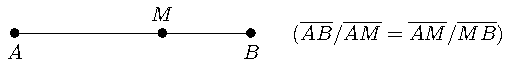
\includegraphics[width=0.55\textwidth]{gold.pdf}
    \caption{Divisão áurea de um segmento}
\label{fig:div_gold}
\end{figure}

O valor da razão entre esses segmentos que realiza isso é dada pela equação \ref{eq:u}.
\begin{equation}
u = \frac{\sqrt{5}-1}{2}  \approx 0.6180
\label{eq:u}
\end{equation}

O método da seção áurea é bastante parecido com o método de Fibonacci. A diferença reside no fato de que os pontos centrais $x_2$ e $x_3$ são determinados através da razão áurea da equação \ref{eq:u}. Além disso, nesse caso, não se determina um número desejado de reduções como no método de Fibonacci, mas sim uma tolerância $\varepsilon \in  \mathbb{R}$ para o intervalo final.

De fato, um incoveniente do algoritmo de Fibonacci está relacionado à necessidade de se conhecer a priori o número total de reduções e o índice k associado, ao passo que, no método da divisão áurea, isso não é necessário. Na verdade, demonstra-se inclusive que, se o número de reduções prevista no algoritmo de Fibonacci for grande (n>10), a primeira redução do método de Fibonacci corresponde justamente à divisão áurea.\\

O diagrama de fluxo da implentação do algoritmo da seção áurea é apresentado na figura \ref{fig:gold}.

\begin{figure}[h!]
\centering
\scalebox{.85}{% Define block styles
\tikzstyle{decision} = [diamond, draw, fill=red!20, 
    text width=4.5em, text centered, node distance=3cm, inner sep=0pt]
\tikzstyle{block} = [rectangle, draw, fill=blue!20, 
    text width=9em, text centered, rounded corners, minimum height=1em]
\tikzstyle{block2} = [rectangle, draw, fill=cyan!20, node distance=2.5cm,
    text width=9em, text centered,rounded corners, minimum height=3.5em]
\tikzstyle{line} = [draw, -latex']
\tikzstyle{cloud} = [draw, ellipse,fill=green!20, node distance=2cm,
    minimum height=2em]
    \tikzstyle{io} = [trapezium,trapezium left angle=70,trapezium right angle=-70,minimum height=1cm, draw, fill=yellow!20, text width=5.5em, text badly centered, node distance=2.5cm, inner sep=0pt]
    \tikzstyle{io2} = [trapezium,trapezium left angle=70,trapezium right angle=-70,minimum height=0.5cm, draw, fill=yellow!20, text width=4em, text badly centered, node distance=3.5cm, inner sep=0pt]
    
    
\begin{tikzpicture}[node distance = 2cm, auto]
    % Place nodes
    \node [io] (input) {$I_1: [a\;b]$ \\ $\varepsilon$: toler\^ancia};
    \node [block,below of = input] (init) {$x_1 = a$; $x_4 = b$ \\$L_i = b - a$; $u = \frac{\sqrt{5}-1}{2}$\\$x_2 = u x_1 + (1-u) x_4$\\$x_3 = (1-u)x_1 + ux_4$};
    \node [decision, below of=init] (evaluate) {$f_2 < f_3$};
    \node[below of = evaluate](aux){};
    \node [block2, left of=aux,node distance=3.5cm] (passo7) {$a=x_2$\\ $b=x_4$ \\$L_f = b-a$};
    \node [decision,below of=passo7] (tolerancia) {$L_f < \varepsilon$};
    \node [block2, right of=aux,node distance=3.5cm] (passo6) {$a = x_1$\\ $b = x_3$\\ $L_f = b-a$};
    \node [decision,below of=passo6] (tolerancia2) {$L_f < \varepsilon$};
    \node [block2, below of = tolerancia] (passo7parte2) {$ x_1 = x_2; \,x_2 = x_3$\\$x_3 = (1-u)a+ub$};
    \node [block2, below of = tolerancia2] (passo6parte2) {$x_4 = x_3; \, x_3 = x_2$\\$x_2 = ua+(1-u)b$};
    \node[io2, right of = tolerancia,node distance=3.5cm](out){$I_f:[a\;b]$};
    \node[cloud, below of = out](stop){FIM};
     
        
    % Draw edges
    \path [line] (input) -- (init);
    \path [line] (init) -- (evaluate);
    \path [line] (evaluate.south west) -- node [above]{não} (passo7);
    \path [line] (evaluate.south east) -- node [above] {sim} (passo6);
    \path [line] (passo7) -- (tolerancia);
    \path [line] (passo6) -- (tolerancia2);
    \path [line] (tolerancia) -- node [near start] {não} (passo7parte2);
    \path [line] (tolerancia2) -- node [near start] {não} (passo6parte2);
    \path[line] (tolerancia) -- node [above] {sim} (out);
    \path[line] (tolerancia2) -- node [above] {sim} (out);
    \path[line] (out) -- (stop);
    \draw [line,rounded corners] (passo7parte2.west) -- ++(-0.5,0) |- node[anchor=west] {} (evaluate.west);
    \draw [line,rounded corners] (passo6parte2.east) -- ++(0.5,0) |- node[anchor=east] {} (evaluate.east);
 \end{tikzpicture}}
\caption{Seção Áurea}
\label{fig:gold}
\end{figure}

\subsection{Resultado}

\vspace{0.5cm}

O resultado obtido utilizando a função teste enunciada em \ref{eq:func_obj} é apresentado na figura \ref{fig:aurea}.\\

\begin{figure}[h!]
\centering
\scalebox{.85}{% This file was created by matlab2tikz.
%
%The latest updates can be retrieved from
%  http://www.mathworks.com/matlabcentral/fileexchange/22022-matlab2tikz-matlab2tikz
%where you can also make suggestions and rate matlab2tikz.
%
\definecolor{mycolor1}{rgb}{1.00000,1.00000,0.00000}%
%
\begin{tikzpicture}

\begin{axis}[%
width=4.521in,
height=3.566in,
at={(0.758in,0.481in)},
scale only axis,
separate axis lines,
every outer x axis line/.append style={black},
every x tick label/.append style={font=\color{black}},
xmin=-12.5,
xmax=5,
xlabel={$x$},
xmajorgrids,
every outer y axis line/.append style={black},
every y tick label/.append style={font=\color{black}},
ymin=-2000,
ymax=5000,
ylabel={$f(x)$},
ymajorgrids,
axis background/.style={fill=white},
title={M\'etodo da Seç\~ao \'Aurea: $f(x) = x^4 + 10 x^3$}
]
\addplot [color=blue,solid,line width=2.0pt,forget plot]
  table[row sep=crcr]{%
-12.51	4914.11879001\\
-12.5	4882.8125\\
-12.49	4851.61871001\\
-12.48	4820.53718016\\
-12.47	4789.56767081\\
-12.46	4758.70994256\\
-12.45	4727.96375625\\
-12.44	4697.32887296\\
-12.43	4666.80505401\\
-12.42	4636.39206096\\
-12.41	4606.08965561\\
-12.4	4575.8976\\
-12.39	4545.81565641\\
-12.38	4515.84358736\\
-12.37	4485.98115561\\
-12.36	4456.22812416\\
-12.35	4426.58425625\\
-12.34	4397.04931536\\
-12.33	4367.62306521\\
-12.32	4338.30526976\\
-12.31	4309.09569321\\
-12.3	4279.9941\\
-12.29	4251.00025481\\
-12.28	4222.11392256\\
-12.27	4193.33486841\\
-12.26	4164.66285776\\
-12.25	4136.09765625\\
-12.24	4107.63902976\\
-12.23	4079.28674441\\
-12.22	4051.04056656\\
-12.21	4022.90026281\\
-12.2	3994.8656\\
-12.19	3966.93634521\\
-12.18	3939.11226576\\
-12.17	3911.39312921\\
-12.16	3883.77870336\\
-12.15	3856.26875625\\
-12.14	3828.86305616\\
-12.13	3801.56137161\\
-12.12	3774.36347136\\
-12.11	3747.26912441\\
-12.1	3720.2781\\
-12.09	3693.39016761\\
-12.08	3666.60509696\\
-12.07	3639.92265801\\
-12.06	3613.34262096\\
-12.05	3586.86475625\\
-12.04	3560.48883456\\
-12.03	3534.21462681\\
-12.02	3508.04190416\\
-12.01	3481.97043801\\
-12	3456\\
-11.99	3430.13036201\\
-11.98	3404.36129616\\
-11.97	3378.69257481\\
-11.96	3353.12397056\\
-11.95	3327.65525625\\
-11.94	3302.28620496\\
-11.93	3277.01659001\\
-11.92	3251.84618496\\
-11.91	3226.77476361\\
-11.9	3201.8021\\
-11.89	3176.92796841\\
-11.88	3152.15214336\\
-11.87	3127.47439961\\
-11.86	3102.89451216\\
-11.85	3078.41225625\\
-11.84	3054.02740736\\
-11.83	3029.73974121\\
-11.82	3005.54903376\\
-11.81	2981.45506121\\
-11.8	2957.45760000001\\
-11.79	2933.55642681\\
-11.78	2909.75131856\\
-11.77	2886.04205241\\
-11.76	2862.42840576\\
-11.75	2838.91015625\\
-11.74	2815.48708176\\
-11.73	2792.15896041\\
-11.72	2768.92557056\\
-11.71	2745.78669081\\
-11.7	2722.7421\\
-11.69	2699.79157721\\
-11.68	2676.93490176\\
-11.67	2654.17185321\\
-11.66	2631.50221136\\
-11.65	2608.92575625\\
-11.64	2586.44226816\\
-11.63	2564.05152761\\
-11.62	2541.75331536\\
-11.61	2519.54741241\\
-11.6	2497.4336\\
-11.59	2475.41165961\\
-11.58	2453.48137296\\
-11.57	2431.64252201\\
-11.56	2409.89488896\\
-11.55	2388.23825625\\
-11.54	2366.67240656\\
-11.53	2345.19712281\\
-11.52	2323.81218816\\
-11.51	2302.51738601\\
-11.5	2281.3125\\
-11.49	2260.19731401\\
-11.48	2239.17161216\\
-11.47	2218.23517881\\
-11.46	2197.38779856\\
-11.45	2176.62925625\\
-11.44	2155.95933696\\
-11.43	2135.37782601\\
-11.42	2114.88450896\\
-11.41	2094.47917161\\
-11.4	2074.1616\\
-11.39	2053.93158041\\
-11.38	2033.78889936\\
-11.37	2013.73334361\\
-11.36	1993.76470016\\
-11.35	1973.88275625\\
-11.34	1954.08729936\\
-11.33	1934.37811721\\
-11.32	1914.75499776\\
-11.31	1895.21772921\\
-11.3	1875.7661\\
-11.29	1856.39989881\\
-11.28	1837.11891456\\
-11.27	1817.92293641\\
-11.26	1798.81175376\\
-11.25	1779.78515625\\
-11.24	1760.84293376\\
-11.23	1741.98487641\\
-11.22	1723.21077456\\
-11.21	1704.52041881\\
-11.2	1685.9136\\
-11.19	1667.39010921\\
-11.18	1648.94973776\\
-11.17	1630.59227721\\
-11.16	1612.31751936\\
-11.15	1594.12525625\\
-11.14	1576.01528016\\
-11.13	1557.98738361\\
-11.12	1540.04135936\\
-11.11	1522.17700041\\
-11.1	1504.3941\\
-11.09	1486.69245161\\
-11.08	1469.07184896\\
-11.07	1451.53208601\\
-11.06	1434.07295696\\
-11.05	1416.69425625\\
-11.04	1399.39577856\\
-11.03	1382.17731881\\
-11.02	1365.03867216\\
-11.01	1347.97963401\\
-11	1331\\
-10.99	1314.09956601\\
-10.98	1297.27812816\\
-10.97	1280.53548281\\
-10.96	1263.87142656\\
-10.95	1247.28575625\\
-10.94	1230.77826896\\
-10.93	1214.34876201\\
-10.92	1197.99703296\\
-10.91	1181.72287961\\
-10.9	1165.5261\\
-10.89	1149.40649241\\
-10.88	1133.36385536\\
-10.87	1117.39798761\\
-10.86	1101.50868816\\
-10.85	1085.69575625\\
-10.84	1069.95899136\\
-10.83	1054.29819321\\
-10.82	1038.71316176\\
-10.81	1023.20369721\\
-10.8	1007.7696\\
-10.79	992.410670809999\\
-10.78	977.126710559998\\
-10.77	961.917520409999\\
-10.76	946.78290176\\
-10.75	931.72265625\\
-10.74	916.736585760002\\
-10.73	901.82449241\\
-10.72	886.986178559999\\
-10.71	872.221446809999\\
-10.7	857.5301\\
-10.69	842.911941209997\\
-10.68	828.366773759997\\
-10.67	813.89440121\\
-10.66	799.49462736\\
-10.65	785.167256250001\\
-10.64	770.912092159999\\
-10.63	756.728939609999\\
-10.62	742.61760336\\
-10.61	728.577888409998\\
-10.6	714.6096\\
-10.59	700.71254361\\
-10.58	686.88652496\\
-10.57	673.13135001\\
-10.56	659.446824960001\\
-10.55	645.83275625\\
-10.54	632.28895056\\
-10.53	618.81521481\\
-10.52	605.411356160001\\
-10.51	592.07718201\\
-10.5	578.8125\\
-10.49	565.617118010001\\
-10.48	552.49084416\\
-10.47	539.433486809998\\
-10.46	526.444854560001\\
-10.45	513.524756249999\\
-10.44	500.67300096\\
-10.43	487.889398009998\\
-10.42	475.173756960001\\
-10.41	462.52588761\\
-10.4	449.945600000003\\
-10.39	437.432704410001\\
-10.38	424.987011360001\\
-10.37	412.608331609998\\
-10.36	400.29647616\\
-10.35	388.051256249999\\
-10.34	375.872483359999\\
-10.33	363.759969210001\\
-10.32	351.71352576\\
-10.31	339.732965209998\\
-10.3	327.818099999999\\
-10.29	315.968742809999\\
-10.28	304.18470656\\
-10.27	292.465804409998\\
-10.26	280.811849759999\\
-10.25	269.22265625\\
-10.24	257.698037759998\\
-10.23	246.23780841\\
-10.22	234.841782559999\\
-10.21	223.50977481\\
-10.2	212.241599999999\\
-10.19	201.03707321\\
-10.18	189.896009760001\\
-10.17	178.81822521\\
-10.16	167.803535359999\\
-10.15	156.851756249998\\
-10.14	145.962704160002\\
-10.13	135.136195609999\\
-10.12	124.372047359999\\
-10.11	113.670076410001\\
-10.1	103.0301\\
-10.09	92.4519356099991\\
-10.08	81.9354009600011\\
-10.07	71.4803140099993\\
-10.06	61.0864929599975\\
-10.05	50.753756250002\\
-10.04	40.4819225599986\\
-10.03	30.2708108099978\\
-10.02	20.1202401600003\\
-10.01	10.0300300100007\\
-10	0\\
-9.99	-9.9700299899996\\
-9.98	-19.8802398400003\\
-9.97	-29.7308091900013\\
-9.96	-39.5219174400008\\
-9.95	-49.2537437500014\\
-9.94	-58.9264670400007\\
-9.93	-68.5402659899992\\
-9.92	-78.0953190399996\\
-9.91	-87.5918043900001\\
-9.9	-97.0298999999995\\
-9.89	-106.409783589999\\
-9.88	-115.731632640001\\
-9.87	-124.995624390001\\
-9.86	-134.201935840001\\
-9.85	-143.350743750001\\
-9.84	-152.442224639999\\
-9.83	-161.476554789999\\
-9.82	-170.453910239999\\
-9.81	-179.374466790003\\
-9.8	-188.238399999998\\
-9.79	-197.04588519\\
-9.78	-205.797097440001\\
-9.77	-214.492211590001\\
-9.76	-223.13140224\\
-9.75	-231.71484375\\
-9.74	-240.24271024\\
-9.73	-248.715175589999\\
-9.72	-257.13241344\\
-9.71	-265.494597190002\\
-9.7	-273.8019\\
-9.69	-282.05449479\\
-9.68	-290.25255424\\
-9.67	-298.39625079\\
-9.66	-306.485756640001\\
-9.65	-314.521243749999\\
-9.64	-322.502883839999\\
-9.63	-330.43084839\\
-9.62	-338.30530864\\
-9.61	-346.12643559\\
-9.6	-353.894399999999\\
-9.59	-361.609372390001\\
-9.58	-369.271523040001\\
-9.57	-376.881021990001\\
-9.56	-384.438039040002\\
-9.55	-391.942743749998\\
-9.54	-399.395305440001\\
-9.53	-406.795893190001\\
-9.52	-414.14467584\\
-9.51	-421.44182199\\
-9.5	-428.6875\\
-9.49	-435.881877990001\\
-9.48	-443.025123840001\\
-9.47	-450.117405190001\\
-9.46	-457.15888944\\
-9.45	-464.149743750001\\
-9.44	-471.090135040001\\
-9.43	-477.980229989999\\
-9.42	-484.820195040001\\
-9.41	-491.61019639\\
-9.4	-498.350399999999\\
-9.39	-505.040971590001\\
-9.38	-511.682076640001\\
-9.37	-518.273880390001\\
-9.36	-524.816547840001\\
-9.35	-531.310243750001\\
-9.34	-537.75513264\\
-9.33	-544.151378789999\\
-9.32	-550.49914624\\
-9.31	-556.798598790001\\
-9.3	-563.049899999999\\
-9.29	-569.25321319\\
-9.28	-575.40870144\\
-9.27	-581.51652759\\
-9.26	-587.57685424\\
-9.25	-593.58984375\\
-9.24	-599.55565824\\
-9.23	-605.47445959\\
-9.22	-611.346409440001\\
-9.21	-617.171669190001\\
-9.2	-622.950400000002\\
-9.19	-628.68276279\\
-9.18	-634.36891824\\
-9.17	-640.00902679\\
-9.16	-645.603248639999\\
-9.15	-651.151743750001\\
-9.14	-656.65467184\\
-9.13	-662.112192390001\\
-9.12	-667.52446464\\
-9.11	-672.89164759\\
-9.1	-678.213900000001\\
-9.09	-683.491380390001\\
-9.08	-688.724247039999\\
-9.07	-693.91265799\\
-9.06	-699.05677104\\
-9.05	-704.15674375\\
-9.04	-709.212733439999\\
-9.03	-714.224897190001\\
-9.02	-719.19339184\\
-9.01	-724.11837399\\
-9	-729\\
-8.99	-733.83842599\\
-8.98	-738.63380784\\
-8.97	-743.386301189999\\
-8.96	-748.096061440001\\
-8.95	-752.76324375\\
-8.94	-757.38800304\\
-8.93	-761.97049399\\
-8.92	-766.51087104\\
-8.91	-771.009288390001\\
-8.9	-775.465899999999\\
-8.89	-779.88085959\\
-8.88	-784.254320640001\\
-8.87	-788.58643639\\
-8.86	-792.87735984\\
-8.85	-797.12724375\\
-8.84	-801.33624064\\
-8.83	-805.50450279\\
-8.82	-809.63218224\\
-8.81	-813.71943079\\
-8.8	-817.7664\\
-8.79	-821.77324119\\
-8.78	-825.74010544\\
-8.77	-829.66714359\\
-8.76	-833.554506240001\\
-8.75	-837.40234375\\
-8.74	-841.21080624\\
-8.73	-844.980043590001\\
-8.72	-848.71020544\\
-8.71	-852.401441190001\\
-8.7	-856.0539\\
-8.69	-859.66773079\\
-8.68	-863.243082239999\\
-8.67	-866.78010279\\
-8.66	-870.27894064\\
-8.65	-873.739743749999\\
-8.64	-877.162659840001\\
-8.63	-880.547836389999\\
-8.62	-883.895420640001\\
-8.61	-887.20555959\\
-8.6	-890.4784\\
-8.59	-893.714088389999\\
-8.58	-896.912771040001\\
-8.57	-900.074593990001\\
-8.56	-903.19970304\\
-8.55	-906.28824375\\
-8.54	-909.340361439999\\
-8.53	-912.356201190001\\
-8.52	-915.33590784\\
-8.51	-918.27962599\\
-8.5	-921.1875\\
-8.49	-924.059673990001\\
-8.48	-926.89629184\\
-8.47	-929.69749719\\
-8.46	-932.46343344\\
-8.45	-935.194243750001\\
-8.44	-937.890071039999\\
-8.43	-940.55105799\\
-8.42	-943.17734704\\
-8.41	-945.76908039\\
-8.4	-948.326400000001\\
-8.39	-950.84944759\\
-8.38	-953.33836464\\
-8.37	-955.793292390001\\
-8.36	-958.21437184\\
-8.35	-960.60174375\\
-8.34	-962.95554864\\
-8.33	-965.27592679\\
-8.32	-967.56301824\\
-8.31	-969.816962790001\\
-8.3	-972.0379\\
-8.29	-974.22596919\\
-8.28	-976.38130944\\
-8.27	-978.50405959\\
-8.26	-980.59435824\\
-8.25	-982.65234375\\
-8.24	-984.67815424\\
-8.23	-986.67192759\\
-8.22	-988.63380144\\
-8.21	-990.56391319\\
-8.2	-992.4624\\
-8.19	-994.32939879\\
-8.18	-996.165046239999\\
-8.17	-997.969478790001\\
-8.16	-999.742832640001\\
-8.15	-1001.48524375\\
-8.14	-1003.19684784\\
-8.13	-1004.87778039\\
-8.12	-1006.52817664\\
-8.11	-1008.14817159\\
-8.1	-1009.7379\\
-8.09	-1011.29749639\\
-8.08	-1012.82709504\\
-8.07	-1014.32682999\\
-8.06	-1015.79683504\\
-8.05	-1017.23724375\\
-8.04	-1018.64818944\\
-8.03	-1020.02980519\\
-8.02	-1021.38222384\\
-8.01	-1022.70557799\\
-8	-1024\\
-7.99	-1025.26562199\\
-7.98	-1026.50257584\\
-7.97	-1027.71099319\\
-7.96	-1028.89100544\\
-7.95	-1030.04274375\\
-7.94	-1031.16633904\\
-7.93	-1032.26192199\\
-7.92	-1033.32962304\\
-7.91	-1034.36957239\\
-7.9	-1035.3819\\
-7.89	-1036.36673559\\
-7.88	-1037.32420864\\
-7.87	-1038.25444839\\
-7.86	-1039.15758384\\
-7.85	-1040.03374375\\
-7.84	-1040.88305664\\
-7.83	-1041.70565079\\
-7.82	-1042.50165424\\
-7.81	-1043.27119479\\
-7.8	-1044.0144\\
-7.79	-1044.73139719\\
-7.78	-1045.42231344\\
-7.77	-1046.08727559\\
-7.76	-1046.72641024\\
-7.75	-1047.33984375\\
-7.74	-1047.92770224\\
-7.73	-1048.49011159\\
-7.72	-1049.02719744\\
-7.71	-1049.53908519\\
-7.7	-1050.0259\\
-7.69	-1050.48776679\\
-7.68	-1050.92481024\\
-7.67	-1051.33715479\\
-7.66	-1051.72492464\\
-7.65	-1052.08824375\\
-7.64	-1052.42723584\\
-7.63	-1052.74202439\\
-7.62	-1053.03273264\\
-7.61	-1053.29948359\\
-7.6	-1053.5424\\
-7.59	-1053.76160439\\
-7.58	-1053.95721904\\
-7.57	-1054.12936599\\
-7.56	-1054.27816704\\
-7.55	-1054.40374375\\
-7.54	-1054.50621744\\
-7.53	-1054.58570919\\
-7.52	-1054.64233984\\
-7.51	-1054.67622999\\
-7.5	-1054.6875\\
-7.49	-1054.67626999\\
-7.48	-1054.64265984\\
-7.47	-1054.58678919\\
-7.46	-1054.50877744\\
-7.45	-1054.40874375\\
-7.44	-1054.28680704\\
-7.43	-1054.14308599\\
-7.42	-1053.97769904\\
-7.41	-1053.79076439\\
-7.4	-1053.5824\\
-7.39	-1053.35272359\\
-7.38	-1053.10185264\\
-7.37	-1052.82990439\\
-7.36	-1052.53699584\\
-7.35	-1052.22324375\\
-7.34	-1051.88876464\\
-7.33	-1051.53367479\\
-7.32	-1051.15809024\\
-7.31	-1050.76212679\\
-7.3	-1050.3459\\
-7.29	-1049.90952519\\
-7.28	-1049.45311744\\
-7.27	-1048.97679159\\
-7.26	-1048.48066224\\
-7.25	-1047.96484375\\
-7.24	-1047.42945024\\
-7.23	-1046.87459559\\
-7.22	-1046.30039344\\
-7.21	-1045.70695719\\
-7.2	-1045.0944\\
-7.19	-1044.46283479\\
-7.18	-1043.81237424\\
-7.17	-1043.14313079\\
-7.16	-1042.45521664\\
-7.15	-1041.74874375\\
-7.14	-1041.02382384\\
-7.13	-1040.28056839\\
-7.12	-1039.51908864\\
-7.11	-1038.73949559\\
-7.1	-1037.9419\\
-7.09	-1037.12641239\\
-7.08	-1036.29314304\\
-7.07	-1035.44220199\\
-7.06	-1034.57369904\\
-7.05	-1033.68774375\\
-7.04	-1032.78444544\\
-7.03	-1031.86391319\\
-7.02	-1030.92625584\\
-7.01	-1029.97158199\\
-7	-1029\\
-6.99	-1028.01161799\\
-6.98	-1027.00654384\\
-6.97	-1025.98488519\\
-6.96	-1024.94674944\\
-6.95	-1023.89224375\\
-6.94	-1022.82147504\\
-6.93	-1021.73454999\\
-6.92	-1020.63157504\\
-6.91	-1019.51265639\\
-6.9	-1018.3779\\
-6.89	-1017.22741159\\
-6.88	-1016.06129664\\
-6.87	-1014.87966039\\
-6.86	-1013.68260784\\
-6.85	-1012.47024375\\
-6.84	-1011.24267264\\
-6.83	-1009.99999879\\
-6.82	-1008.74232624\\
-6.81	-1007.46975879\\
-6.8	-1006.1824\\
-6.79	-1004.88035319\\
-6.78	-1003.56372144\\
-6.77	-1002.23260759\\
-6.76	-1000.88711424\\
-6.75	-999.52734375\\
-6.74	-998.15339824\\
-6.73	-996.76537959\\
-6.72	-995.36338944\\
-6.71	-993.94752919\\
-6.7	-992.5179\\
-6.69	-991.07460279\\
-6.68	-989.61773824\\
-6.67	-988.14740679\\
-6.66	-986.66370864\\
-6.65	-985.16674375\\
-6.64	-983.65661184\\
-6.63	-982.13341239\\
-6.62	-980.59724464\\
-6.61	-979.04820759\\
-6.6	-977.4864\\
-6.59	-975.91192039\\
-6.58	-974.32486704\\
-6.57	-972.72533799\\
-6.56	-971.11343104\\
-6.55	-969.48924375\\
-6.54	-967.85287344\\
-6.53	-966.20441719\\
-6.52	-964.54397184\\
-6.51	-962.87163399\\
-6.5	-961.1875\\
-6.49	-959.49166599\\
-6.48	-957.78422784\\
-6.47	-956.06528119\\
-6.46	-954.33492144\\
-6.45	-952.59324375\\
-6.44	-950.84034304\\
-6.43	-949.07631399\\
-6.42	-947.30125104\\
-6.41	-945.51524839\\
-6.4	-943.7184\\
-6.39	-941.91079959\\
-6.38	-940.09254064\\
-6.37	-938.26371639\\
-6.36	-936.42441984\\
-6.35	-934.57474375\\
-6.34	-932.71478064\\
-6.33	-930.84462279\\
-6.32	-928.96436224\\
-6.31	-927.07409079\\
-6.3	-925.1739\\
-6.29	-923.26388119\\
-6.28	-921.34412544\\
-6.27	-919.41472359\\
-6.26	-917.47576624\\
-6.25	-915.52734375\\
-6.24	-913.56954624\\
-6.23	-911.60246359\\
-6.22	-909.62618544\\
-6.21	-907.64080119\\
-6.2	-905.6464\\
-6.19	-903.64307079\\
-6.18	-901.63090224\\
-6.17	-899.60998279\\
-6.16	-897.58040064\\
-6.15	-895.54224375\\
-6.14	-893.49559984\\
-6.13	-891.44055639\\
-6.12	-889.37720064\\
-6.11	-887.30561959\\
-6.1	-885.2259\\
-6.09	-883.13812839\\
-6.08	-881.04239104\\
-6.07	-878.93877399\\
-6.06	-876.82736304\\
-6.05	-874.70824375\\
-6.04	-872.58150144\\
-6.03	-870.44722119\\
-6.02	-868.30548784\\
-6.01	-866.15638599\\
-6	-864\\
-5.99	-861.83641399\\
-5.98	-859.66571184\\
-5.97	-857.48797719\\
-5.96	-855.30329344\\
-5.95	-853.11174375\\
-5.94	-850.91341104\\
-5.93	-848.70837799\\
-5.92	-846.49672704\\
-5.91	-844.27854039\\
-5.9	-842.0539\\
-5.89	-839.82288759\\
-5.88	-837.58558464\\
-5.87	-835.34207239\\
-5.86	-833.09243184\\
-5.85	-830.83674375\\
-5.84	-828.57508864\\
-5.83	-826.30754679\\
-5.82	-824.03419824\\
-5.81	-821.75512279\\
-5.8	-819.4704\\
-5.79	-817.18010919\\
-5.78	-814.88432944\\
-5.77	-812.58313959\\
-5.76	-810.27661824\\
-5.75	-807.96484375\\
-5.74	-805.64789424\\
-5.73	-803.32584759\\
-5.72	-800.99878144\\
-5.71	-798.66677319\\
-5.7	-796.3299\\
-5.69	-793.98823879\\
-5.68	-791.64186624\\
-5.67	-789.29085879\\
-5.66	-786.93529264\\
-5.65	-784.57524375\\
-5.64	-782.21078784\\
-5.63	-779.84200039\\
-5.62	-777.46895664\\
-5.61	-775.09173159\\
-5.6	-772.7104\\
-5.59	-770.32503639\\
-5.58	-767.93571504\\
-5.57	-765.54250999\\
-5.56	-763.14549504\\
-5.55	-760.74474375\\
-5.54	-758.34032944\\
-5.53	-755.93232519\\
-5.52	-753.52080384\\
-5.51	-751.10583799\\
-5.5	-748.6875\\
-5.49	-746.26586199\\
-5.48	-743.84099584\\
-5.47	-741.41297319\\
-5.46	-738.98186544\\
-5.45	-736.54774375\\
-5.44	-734.11067904\\
-5.43	-731.67074199\\
-5.42	-729.22800304\\
-5.41	-726.78253239\\
-5.4	-724.3344\\
-5.39	-721.88367559\\
-5.38	-719.43042864\\
-5.37	-716.97472839\\
-5.36	-714.51664384\\
-5.35	-712.05624375\\
-5.34	-709.59359664\\
-5.33	-707.12877079\\
-5.32	-704.66183424\\
-5.31	-702.19285479\\
-5.3	-699.7219\\
-5.29	-697.24903719\\
-5.28	-694.77433344\\
-5.27	-692.29785559\\
-5.26	-689.81967024\\
-5.25	-687.33984375\\
-5.24	-684.85844224\\
-5.23	-682.37553159\\
-5.22	-679.89117744\\
-5.21	-677.40544519\\
-5.2	-674.9184\\
-5.19	-672.43010679\\
-5.18	-669.94063024\\
-5.17	-667.45003479\\
-5.16	-664.95838464\\
-5.15	-662.46574375\\
-5.14	-659.97217584\\
-5.13	-657.47774439\\
-5.12	-654.98251264\\
-5.11	-652.48654359\\
-5.1	-649.9899\\
-5.09	-647.49264439\\
-5.08	-644.99483904\\
-5.07	-642.49654599\\
-5.06	-639.99782704\\
-5.05	-637.49874375\\
-5.04	-634.99935744\\
-5.03	-632.49972919\\
-5.02	-629.99991984\\
-5.01	-627.49998999\\
-5	-625\\
-4.99	-622.50000999\\
-4.98	-620.00007984\\
-4.97	-617.50026919\\
-4.96	-615.00063744\\
-4.95	-612.50124375\\
-4.94	-610.00214704\\
-4.93	-607.50340599\\
-4.92	-605.00507904\\
-4.91	-602.50722439\\
-4.9	-600.0099\\
-4.89	-597.51316359\\
-4.88	-595.01707264\\
-4.87	-592.52168439\\
-4.86	-590.02705584\\
-4.85	-587.53324375\\
-4.84	-585.04030464\\
-4.83	-582.54829479\\
-4.82	-580.05727024\\
-4.81	-577.56728679\\
-4.8	-575.0784\\
-4.79	-572.59066519\\
-4.78	-570.10413744\\
-4.77	-567.61887159\\
-4.76	-565.13492224\\
-4.75	-562.65234375\\
-4.74	-560.17119024\\
-4.73	-557.69151559\\
-4.72	-555.21337344\\
-4.71	-552.73681719\\
-4.7	-550.2619\\
-4.69	-547.78867479\\
-4.68	-545.31719424\\
-4.67	-542.84751079\\
-4.66	-540.37967664\\
-4.65	-537.91374375\\
-4.64	-535.44976384\\
-4.63	-532.98778839\\
-4.62	-530.52786864\\
-4.61	-528.07005559\\
-4.6	-525.6144\\
-4.59	-523.16095239\\
-4.58	-520.70976304\\
-4.57	-518.26088199\\
-4.56	-515.81435904\\
-4.55	-513.37024375\\
-4.54	-510.92858544\\
-4.53	-508.48943319\\
-4.52	-506.05283584\\
-4.51	-503.61884199\\
-4.5	-501.1875\\
-4.49	-498.75885799\\
-4.48	-496.33296384\\
-4.47	-493.90986519\\
-4.46	-491.48960944\\
-4.45	-489.07224375\\
-4.44	-486.65781504\\
-4.43	-484.24636999\\
-4.42	-481.83795504\\
-4.41	-479.43261639\\
-4.4	-477.0304\\
-4.39	-474.63135159\\
-4.38	-472.23551664\\
-4.37	-469.84294039\\
-4.36	-467.45366784\\
-4.35	-465.06774375\\
-4.34	-462.68521264\\
-4.33	-460.30611879\\
-4.32	-457.93050624\\
-4.31	-455.55841879\\
-4.3	-453.1899\\
-4.29	-450.82499319\\
-4.28	-448.46374144\\
-4.27	-446.10618759\\
-4.26	-443.75237424\\
-4.25	-441.40234375\\
-4.24	-439.05613824\\
-4.23	-436.71379959\\
-4.22	-434.37536944\\
-4.21	-432.04088919\\
-4.2	-429.7104\\
-4.19	-427.38394279\\
-4.18	-425.06155824\\
-4.17	-422.74328679\\
-4.16	-420.42916864\\
-4.15	-418.11924375\\
-4.14	-415.81355184\\
-4.13	-413.51213239\\
-4.12	-411.21502464\\
-4.11	-408.92226759\\
-4.1	-406.6339\\
-4.09	-404.34996039\\
-4.08	-402.07048704\\
-4.07	-399.79551799\\
-4.06	-397.52509104\\
-4.05	-395.25924375\\
-4.04	-392.99801344\\
-4.03	-390.74143719\\
-4.02	-388.48955184\\
-4.01	-386.24239399\\
-4	-384\\
-3.99	-381.76240599\\
-3.98	-379.52964784\\
-3.97	-377.30176119\\
-3.96	-375.07878144\\
-3.95	-372.86074375\\
-3.94	-370.64768304\\
-3.93	-368.43963399\\
-3.92	-366.23663104\\
-3.91	-364.03870839\\
-3.9	-361.8459\\
-3.89	-359.65823959\\
-3.88	-357.47576064\\
-3.87	-355.29849639\\
-3.86	-353.12647984\\
-3.85	-350.95974375\\
-3.84	-348.79832064\\
-3.83	-346.64224279\\
-3.82	-344.49154224\\
-3.81	-342.34625079\\
-3.8	-340.2064\\
-3.79	-338.07202119\\
-3.78	-335.94314544\\
-3.77	-333.81980359\\
-3.76	-331.70202624\\
-3.75	-329.58984375\\
-3.74	-327.48328624\\
-3.73	-325.38238359\\
-3.72	-323.28716544\\
-3.71	-321.19766119\\
-3.7	-319.1139\\
-3.69	-317.03591079\\
-3.68	-314.96372224\\
-3.67	-312.89736279\\
-3.66	-310.83686064\\
-3.65	-308.78224375\\
-3.64	-306.73353984\\
-3.63	-304.69077639\\
-3.62	-302.65398064\\
-3.61	-300.62317959\\
-3.6	-298.5984\\
-3.59	-296.57966839\\
-3.58	-294.56701104\\
-3.57	-292.56045399\\
-3.56	-290.56002304\\
-3.55	-288.56574375\\
-3.54	-286.57764144\\
-3.53	-284.59574119\\
-3.52	-282.62006784\\
-3.51	-280.65064599\\
-3.5	-278.6875\\
-3.49	-276.73065399\\
-3.48	-274.78013184\\
-3.47	-272.83595719\\
-3.46	-270.89815344\\
-3.45	-268.96674375\\
-3.44	-267.04175104\\
-3.43	-265.12319799\\
-3.42	-263.21110704\\
-3.41	-261.30550039\\
-3.4	-259.4064\\
-3.39	-257.51382759\\
-3.38	-255.62780464\\
-3.37	-253.74835239\\
-3.36	-251.87549184\\
-3.35	-250.00924375\\
-3.34	-248.14962864\\
-3.33	-246.29666679\\
-3.32	-244.45037824\\
-3.31	-242.61078279\\
-3.3	-240.7779\\
-3.29	-238.95174919\\
-3.28	-237.13234944\\
-3.27	-235.31971959\\
-3.26	-233.51387824\\
-3.25	-231.71484375\\
-3.24	-229.92263424\\
-3.23	-228.13726759\\
-3.22	-226.35876144\\
-3.21	-224.58713319\\
-3.2	-222.8224\\
-3.19	-221.06457879\\
-3.18	-219.31368624\\
-3.17	-217.56973879\\
-3.16	-215.83275264\\
-3.15	-214.10274375\\
-3.14	-212.37972784\\
-3.13	-210.66372039\\
-3.12	-208.95473664\\
-3.11	-207.25279159\\
-3.1	-205.5579\\
-3.09	-203.87007639\\
-3.08	-202.18933504\\
-3.07	-200.51568999\\
-3.06	-198.84915504\\
-3.05	-197.18974375\\
-3.04	-195.53746944\\
-3.03	-193.89234519\\
-3.02	-192.25438384\\
-3.01	-190.62359799\\
-3	-189\\
-2.99	-187.38360199\\
-2.98	-185.77441584\\
-2.97	-184.17245319\\
-2.96	-182.57772544\\
-2.95	-180.99024375\\
-2.94	-179.41001904\\
-2.93	-177.83706199\\
-2.92	-176.27138304\\
-2.91	-174.71299239\\
-2.9	-173.1619\\
-2.89	-171.61811559\\
-2.88	-170.08164864\\
-2.87	-168.55250839\\
-2.86	-167.03070384\\
-2.85	-165.51624375\\
-2.84	-164.00913664\\
-2.83	-162.50939079\\
-2.82	-161.01701424\\
-2.81	-159.53201479\\
-2.8	-158.0544\\
-2.79	-156.58417719\\
-2.78	-155.12135344\\
-2.77	-153.66593559\\
-2.76	-152.21793024\\
-2.75	-150.77734375\\
-2.74	-149.34418224\\
-2.73	-147.91845159\\
-2.72	-146.50015744\\
-2.71	-145.08930519\\
-2.7	-143.6859\\
-2.69	-142.28994679\\
-2.68	-140.90145024\\
-2.67	-139.52041479\\
-2.66	-138.14684464\\
-2.65	-136.78074375\\
-2.64	-135.42211584\\
-2.63	-134.07096439\\
-2.62	-132.72729264\\
-2.61	-131.39110359\\
-2.6	-130.0624\\
-2.59	-128.74118439\\
-2.58	-127.42745904\\
-2.57	-126.12122599\\
-2.56	-124.82248704\\
-2.55	-123.53124375\\
-2.54	-122.24749744\\
-2.53	-120.97124919\\
-2.52	-119.70249984\\
-2.51	-118.44124999\\
-2.5	-117.1875\\
-2.49	-115.94124999\\
-2.48	-114.70249984\\
-2.47	-113.47124919\\
-2.46	-112.24749744\\
-2.45	-111.03124375\\
-2.44	-109.82248704\\
-2.43	-108.62122599\\
-2.42	-107.42745904\\
-2.41	-106.24118439\\
-2.4	-105.0624\\
-2.39	-103.89110359\\
-2.38	-102.72729264\\
-2.37	-101.57096439\\
-2.36	-100.42211584\\
-2.35	-99.2807437500001\\
-2.34	-98.1468446400001\\
-2.33	-97.02041479\\
-2.32	-95.90145024\\
-2.31	-94.7899467900001\\
-2.3	-93.6859000000001\\
-2.29	-92.58930519\\
-2.28	-91.50015744\\
-2.27	-90.41845159\\
-2.26	-89.3441822400001\\
-2.25	-88.27734375\\
-2.24	-87.21793024\\
-2.23	-86.16593559\\
-2.22	-85.1213534400001\\
-2.21	-84.08417719\\
-2.2	-83.0544\\
-2.19	-82.03201479\\
-2.18	-81.0170142400001\\
-2.17	-80.00939079\\
-2.16	-79.00913664\\
-2.15	-78.01624375\\
-2.14	-77.0307038400001\\
-2.13	-76.0525083900001\\
-2.12	-75.08164864\\
-2.11	-74.11811559\\
-2.1	-73.1619000000001\\
-2.09	-72.2129923900001\\
-2.08	-71.27138304\\
-2.07	-70.33706199\\
-2.06	-69.4100190400001\\
-2.05	-68.4902437500001\\
-2.04	-67.57772544\\
-2.03	-66.67245319\\
-2.02	-65.77441584\\
-2.01	-64.8836019900001\\
-2	-64\\
-1.99	-63.12359799\\
-1.98	-62.25438384\\
-1.97	-61.3923451900001\\
-1.96	-60.53746944\\
-1.95	-59.68974375\\
-1.94	-58.84915504\\
-1.93	-58.01568999\\
-1.92	-57.18933504\\
-1.91	-56.37007639\\
-1.9	-55.5579\\
-1.89	-54.75279159\\
-1.88	-53.9547366400001\\
-1.87	-53.16372039\\
-1.86	-52.37972784\\
-1.85	-51.60274375\\
-1.84	-50.8327526400001\\
-1.83	-50.06973879\\
-1.82	-49.31368624\\
-1.81	-48.56457879\\
-1.8	-47.8224000000001\\
-1.79	-47.08713319\\
-1.78	-46.35876144\\
-1.77	-45.63726759\\
-1.76	-44.92263424\\
-1.75	-44.21484375\\
-1.74	-43.51387824\\
-1.73	-42.81971959\\
-1.72	-42.13234944\\
-1.71	-41.45174919\\
-1.7	-40.7779\\
-1.69	-40.11078279\\
-1.68	-39.45037824\\
-1.67	-38.79666679\\
-1.66	-38.14962864\\
-1.65	-37.50924375\\
-1.64	-36.87549184\\
-1.63	-36.24835239\\
-1.62	-35.62780464\\
-1.61	-35.01382759\\
-1.6	-34.4064\\
-1.59	-33.80550039\\
-1.58	-33.21110704\\
-1.57	-32.62319799\\
-1.56	-32.04175104\\
-1.55	-31.46674375\\
-1.54	-30.89815344\\
-1.53	-30.33595719\\
-1.52	-29.78013184\\
-1.51	-29.23065399\\
-1.5	-28.6875\\
-1.49	-28.15064599\\
-1.48	-27.62006784\\
-1.47	-27.09574119\\
-1.46	-26.57764144\\
-1.45	-26.06574375\\
-1.44	-25.56002304\\
-1.43	-25.06045399\\
-1.42	-24.56701104\\
-1.41	-24.07966839\\
-1.4	-23.5984\\
-1.39	-23.12317959\\
-1.38	-22.65398064\\
-1.37	-22.19077639\\
-1.36	-21.73353984\\
-1.35	-21.28224375\\
-1.34	-20.83686064\\
-1.33	-20.39736279\\
-1.32	-19.96372224\\
-1.31	-19.53591079\\
-1.3	-19.1139\\
-1.29	-18.69766119\\
-1.28	-18.28716544\\
-1.27	-17.88238359\\
-1.26	-17.48328624\\
-1.25	-17.08984375\\
-1.24	-16.70202624\\
-1.23	-16.31980359\\
-1.22	-15.94314544\\
-1.21	-15.57202119\\
-1.2	-15.2064\\
-1.19	-14.84625079\\
-1.18	-14.49154224\\
-1.17	-14.14224279\\
-1.16	-13.79832064\\
-1.15	-13.45974375\\
-1.14	-13.12647984\\
-1.13	-12.79849639\\
-1.12	-12.47576064\\
-1.11	-12.15823959\\
-1.1	-11.8459\\
-1.09	-11.53870839\\
-1.08	-11.23663104\\
-1.07	-10.93963399\\
-1.06	-10.64768304\\
-1.05	-10.36074375\\
-1.04	-10.07878144\\
-1.03	-9.80176119000001\\
-1.02	-9.52964784000001\\
-1.01	-9.26240599000002\\
-1	-9\\
-0.99	-8.74239399\\
-0.98	-8.48955184000001\\
-0.970000000000001	-8.24143719000002\\
-0.96	-7.99801344\\
-0.95	-7.75924375\\
-0.94	-7.52509104000001\\
-0.930000000000001	-7.29551799000001\\
-0.92	-7.07048704\\
-0.91	-6.84996039\\
-0.9	-6.63390000000001\\
-0.890000000000001	-6.42226759000001\\
-0.88	-6.21502464\\
-0.87	-6.01213239\\
-0.86	-5.81355184000001\\
-0.850000000000001	-5.61924375000001\\
-0.840000000000001	-5.42916864000001\\
-0.83	-5.24328679\\
-0.82	-5.06155824\\
-0.810000000000001	-4.88394279000001\\
-0.800000000000001	-4.71040000000001\\
-0.79	-4.54088919\\
-0.78	-4.37536944\\
-0.77	-4.21379959000001\\
-0.760000000000001	-4.05613824000001\\
-0.75	-3.90234375\\
-0.74	-3.75237424\\
-0.73	-3.60618759000001\\
-0.720000000000001	-3.46374144000001\\
-0.71	-3.32499319\\
-0.7	-3.1899\\
-0.69	-3.05841879000001\\
-0.680000000000001	-2.93050624000001\\
-0.67	-2.80611879\\
-0.66	-2.68521264\\
-0.65	-2.56774375\\
-0.640000000000001	-2.45366784000001\\
-0.63	-2.34294039\\
-0.62	-2.23551664\\
-0.61	-2.13135159\\
-0.600000000000001	-2.03040000000001\\
-0.590000000000001	-1.93261639000001\\
-0.58	-1.83795504\\
-0.57	-1.74636999\\
-0.560000000000001	-1.65781504\\
-0.550000000000001	-1.57224375000001\\
-0.54	-1.48960944\\
-0.53	-1.40986519\\
-0.52	-1.33296384\\
-0.510000000000001	-1.25885799\\
-0.5	-1.1875\\
-0.49	-1.11884199\\
-0.48	-1.05283584\\
-0.470000000000001	-0.989433190000004\\
-0.46	-0.92858544\\
-0.45	-0.870243750000001\\
-0.44	-0.814359040000002\\
-0.430000000000001	-0.760881990000003\\
-0.42	-0.70976304\\
-0.41	-0.660952390000001\\
-0.4	-0.614400000000002\\
-0.390000000000001	-0.570055590000002\\
-0.38	-0.52786864\\
-0.37	-0.48778839\\
-0.36	-0.449763840000001\\
-0.350000000000001	-0.413743750000002\\
-0.340000000000001	-0.379676640000002\\
-0.33	-0.34751079\\
-0.32	-0.317194240000001\\
-0.310000000000001	-0.288674790000001\\
-0.300000000000001	-0.261900000000002\\
-0.29	-0.23681719\\
-0.28	-0.213373440000001\\
-0.27	-0.191515590000001\\
-0.260000000000001	-0.171190240000001\\
-0.25	-0.15234375\\
-0.24	-0.13492224\\
-0.23	-0.118871590000001\\
-0.220000000000001	-0.104137440000001\\
-0.21	-0.0906651899999999\\
-0.2	-0.0784000000000002\\
-0.19	-0.0672867900000004\\
-0.180000000000001	-0.0572702400000006\\
-0.17	-0.0482947899999999\\
-0.16	-0.0403046400000001\\
-0.15	-0.0332437500000002\\
-0.140000000000001	-0.0270558400000003\\
-0.13	-0.0216843899999999\\
-0.12	-0.01707264\\
-0.11	-0.0131635900000001\\
-0.100000000000001	-0.00990000000000016\\
-0.0900000000000007	-0.00722439000000018\\
-0.0800000000000001	-0.00507904000000001\\
-0.0700000000000003	-0.00340599000000004\\
-0.0600000000000005	-0.00214704000000005\\
-0.0500000000000007	-0.00124375000000005\\
-0.04	-0.000637440000000002\\
-0.0300000000000002	-0.000269190000000007\\
-0.0200000000000005	-7.98400000000055e-05\\
-0.0100000000000007	-9.99000000000202e-06\\
0	0\\
0.00999999999999979	1.00099999999994e-05\\
0.0199999999999996	8.01599999999949e-05\\
0.0299999999999994	0.000270809999999983\\
0.04	0.000642560000000002\\
0.0499999999999998	0.00125624999999999\\
0.0599999999999996	0.00217295999999996\\
0.0699999999999994	0.00345400999999991\\
0.0800000000000001	0.00516096000000001\\
0.0899999999999999	0.00735560999999997\\
0.0999999999999996	0.0100999999999999\\
0.109999999999999	0.0134564099999998\\
0.12	0.01748736\\
0.13	0.0222556099999999\\
0.14	0.0278241599999998\\
0.149999999999999	0.0342562499999996\\
0.159999999999999	0.0416153599999994\\
0.17	0.0499652099999999\\
0.18	0.0593697599999997\\
0.19	0.0698932099999994\\
0.199999999999999	0.0815999999999991\\
0.21	0.0945548099999999\\
0.22	0.10882256\\
0.23	0.124468409999999\\
0.239999999999999	0.141557759999999\\
0.25	0.16015625\\
0.26	0.18032976\\
0.27	0.202144409999999\\
0.279999999999999	0.225666559999998\\
0.29	0.25096281\\
0.3	0.2781\\
0.31	0.307145209999999\\
0.319999999999999	0.338165759999998\\
0.33	0.37122921\\
0.34	0.406403359999999\\
0.35	0.443756249999999\\
0.359999999999999	0.483356159999998\\
0.37	0.525271610000001\\
0.38	0.56957136\\
0.39	0.616324409999998\\
0.399999999999999	0.665599999999997\\
0.409999999999999	0.717467609999996\\
0.42	0.77199696\\
0.43	0.829258009999998\\
0.44	0.889320959999997\\
0.449999999999999	0.952256249999995\\
0.46	1.01813456\\
0.47	1.08702681\\
0.48	1.15900416\\
0.489999999999999	1.23413800999999\\
0.5	1.3125\\
0.51	1.39416201\\
0.52	1.47919616\\
0.529999999999999	1.56767480999999\\
0.54	1.65967056\\
0.55	1.75525625\\
0.56	1.85450496\\
0.569999999999999	1.95749000999999\\
0.58	2.06428496\\
0.59	2.17496361\\
0.6	2.2896\\
0.609999999999999	2.40826840999999\\
0.62	2.53104336\\
0.63	2.65799961\\
0.64	2.78921216\\
0.649999999999999	2.92475624999999\\
0.659999999999999	3.06470735999999\\
0.67	3.20914121\\
0.68	3.35813376\\
0.69	3.51176120999999\\
0.699999999999999	3.67009999999999\\
0.71	3.83322681\\
0.72	4.00121856\\
0.73	4.17415240999999\\
0.739999999999999	4.35210575999999\\
0.75	4.53515625\\
0.76	4.72338176\\
0.77	4.91686040999999\\
0.779999999999999	5.11567055999999\\
0.79	5.31989081\\
0.8	5.5296\\
0.81	5.74487720999999\\
0.819999999999999	5.96580175999999\\
0.83	6.19245321\\
0.84	6.42491136\\
0.85	6.66325624999999\\
0.859999999999999	6.90756815999999\\
0.87	7.15792761\\
0.88	7.41441536\\
0.89	7.67711240999999\\
0.899999999999999	7.94609999999999\\
0.91	8.22145961\\
0.92	8.50327296\\
0.93	8.79162200999999\\
0.94	9.08658895999998\\
0.949999999999999	9.38825624999998\\
0.96	9.69670656\\
0.97	10.01202281\\
0.98	10.33428816\\
0.989999999999999	10.66358601\\
1	11\\
1.01	11.34361401\\
1.02	11.69451216\\
1.03	12.05277881\\
1.04	12.41849856\\
1.05	12.79175625\\
1.06	13.17263696\\
1.07	13.56122601\\
1.08	13.95760896\\
1.09	14.36187161\\
1.1	14.7741\\
1.11	15.19438041\\
1.12	15.62279936\\
1.13	16.05944361\\
1.14	16.50440016\\
1.15	16.95775625\\
1.16	17.41959936\\
1.17	17.89001721\\
1.18	18.36909776\\
1.19	18.85692921\\
1.2	19.3536\\
1.21	19.85919881\\
1.22	20.37381456\\
1.23	20.89753641\\
1.24	21.43045376\\
1.25	21.97265625\\
1.26	22.52423376\\
1.27	23.08527641\\
1.28	23.65587456\\
1.29	24.23611881\\
1.3	24.8261\\
1.31	25.42590921\\
1.32	26.03563776\\
1.33	26.65537721\\
1.34	27.28521936\\
1.35	27.92525625\\
1.36	28.57558016\\
1.37	29.23628361\\
1.38	29.90745936\\
1.39	30.58920041\\
1.4	31.2816\\
1.41	31.98475161\\
1.42	32.69874896\\
1.43	33.42368601\\
1.44	34.15965696\\
1.45	34.90675625\\
1.46	35.66507856\\
1.47	36.43471881\\
1.48	37.21577216\\
1.49	38.00833401\\
1.5	38.8125\\
1.51	39.62836601\\
1.52	40.45602816\\
1.53	41.29558281\\
1.54	42.14712656\\
1.55	43.01075625\\
1.56	43.88656896\\
1.57	44.77466201\\
1.58	45.67513296\\
1.59	46.58807961\\
1.6	47.5136\\
1.61	48.45179241\\
1.62	49.40275536\\
1.63	50.36658761\\
1.64	51.34338816\\
1.65	52.33325625\\
1.66	53.33629136\\
1.67	54.35259321\\
1.68	55.38226176\\
1.69	56.42539721\\
1.7	57.4821\\
1.71	58.5524708099999\\
1.72	59.63661056\\
1.73	60.7346204099999\\
1.74	61.84660176\\
1.75	62.97265625\\
1.76	64.11288576\\
1.77	65.26739241\\
1.78	66.43627856\\
1.79	67.6196468099999\\
1.8	68.8176\\
1.81	70.03024121\\
1.82	71.25767376\\
1.83	72.50000121\\
1.84	73.75732736\\
1.85	75.0297562499999\\
1.86	76.31739216\\
1.87	77.62033961\\
1.88	78.93870336\\
1.89	80.27258841\\
1.9	81.6221\\
1.91	82.98734361\\
1.92	84.36842496\\
1.93	85.76545001\\
1.94	87.1785249599999\\
1.95	88.60775625\\
1.96	90.0532505599999\\
1.97	91.51511481\\
1.98	92.9934561599999\\
1.99	94.48838201\\
2	95.9999999999999\\
2.01	97.52841801\\
2.02	99.0737441599999\\
2.03	100.63608681\\
2.04	102.21555456\\
2.05	103.81225625\\
2.06	105.42630096\\
2.07	107.05779801\\
2.08	108.70685696\\
2.09	110.37358761\\
2.1	112.0581\\
2.11	113.76050441\\
2.12	115.48091136\\
2.13	117.21943161\\
2.14	118.97617616\\
2.15	120.75125625\\
2.16	122.54478336\\
2.17	124.35686921\\
2.18	126.18762576\\
2.19	128.03716521\\
2.2	129.9056\\
2.21	131.79304281\\
2.22	133.69960656\\
2.23	135.62540441\\
2.24	137.57054976\\
2.25	139.53515625\\
2.26	141.51933776\\
2.27	143.52320841\\
2.28	145.54688256\\
2.29	147.59047481\\
2.3	149.6541\\
2.31	151.73787321\\
2.32	153.84190976\\
2.33	155.96632521\\
2.34	158.11123536\\
2.35	160.27675625\\
2.36	162.46300416\\
2.37	164.67009561\\
2.38	166.89814736\\
2.39	169.14727641\\
2.4	171.4176\\
2.41	173.70923561\\
2.42	176.02230096\\
2.43	178.35691401\\
2.44	180.71319296\\
2.45	183.09125625\\
2.46	185.49122256\\
2.47	187.91321081\\
2.48	190.35734016\\
2.49	192.82373001\\
2.5	195.3125\\
2.51	197.82377001\\
2.52	200.35766016\\
2.53	202.91429081\\
2.54	205.49378256\\
2.55	208.09625625\\
2.56	210.72183296\\
2.57	213.37063401\\
2.58	216.04278096\\
2.59	218.73839561\\
2.6	221.4576\\
2.61	224.20051641\\
2.62	226.96726736\\
2.63	229.75797561\\
2.64	232.57276416\\
2.65	235.41175625\\
2.66	238.27507536\\
2.67	241.16284521\\
2.68	244.07518976\\
2.69	247.01223321\\
2.7	249.9741\\
2.71	252.96091481\\
2.72	255.97280256\\
2.73	259.00988841\\
2.74	262.07229776\\
2.75	265.16015625\\
2.76	268.27358976\\
2.77	271.41272441\\
2.78	274.57768656\\
2.79	277.76860281\\
2.8	280.9856\\
2.81	284.22880521\\
2.82	287.49834576\\
2.83	290.79434921\\
2.84	294.11694336\\
2.85	297.46625625\\
2.86	300.84241616\\
2.87	304.24555161\\
2.88	307.67579136\\
2.89	311.13326441\\
2.9	314.6181\\
2.91	318.13042761\\
2.92	321.67037696\\
2.93	325.23807801\\
2.94	328.83366096\\
2.95	332.45725625\\
2.96	336.10899456\\
2.97	339.78900681\\
2.98	343.49742416\\
2.99	347.23437801\\
3	351\\
3.01	354.79442201\\
3.02	358.61777616\\
3.03	362.47019481\\
3.04	366.35181056\\
3.05	370.26275625\\
3.06	374.20316496\\
3.07	378.17317001\\
3.08	382.17290496\\
3.09	386.20250361\\
3.1	390.2621\\
3.11	394.35182841\\
3.12	398.47182336\\
3.13	402.62221961\\
3.14	406.80315216\\
3.15	411.01475625\\
3.16	415.25716736\\
3.17	419.53052121\\
3.18	423.83495376\\
3.19	428.17060121\\
3.2	432.5376\\
3.21	436.93608681\\
3.22	441.36619856\\
3.23	445.82807241\\
3.24	450.32184576\\
3.25	454.84765625\\
3.26	459.40564176\\
3.27	463.99594041\\
3.28	468.61869056\\
3.29	473.27403081\\
3.3	477.9621\\
3.31	482.68303721\\
3.32	487.43698176\\
3.33	492.22407321\\
3.34	497.04445136\\
3.35	501.89825625\\
3.36	506.78562816\\
3.37	511.70670761\\
3.38	516.66163536\\
3.39	521.65055241\\
3.4	526.6736\\
3.41	531.73091961\\
3.42	536.82265296\\
3.43	541.94894201\\
3.44	547.10992896\\
3.45	552.30575625\\
3.46	557.53656656\\
3.47	562.80250281\\
3.48	568.10370816\\
3.49	573.44032601\\
3.5	578.8125\\
3.51	584.22037401\\
3.52	589.66409216\\
3.53	595.14379881\\
3.54	600.65963856\\
3.55	606.21175625\\
3.56	611.80029696\\
3.57	617.42540601\\
3.58	623.08722896\\
3.59	628.78591161\\
3.6	634.5216\\
3.61	640.29444041\\
3.62	646.10457936\\
3.63	651.95216361\\
3.64	657.83734016\\
3.65	663.76025625\\
3.66	669.72105936\\
3.67	675.71989721\\
3.68	681.75691776\\
3.69	687.83226921\\
3.7	693.9461\\
3.71	700.09855881\\
3.72	706.28979456\\
3.73	712.51995641\\
3.74	718.78919376\\
3.75	725.09765625\\
3.76	731.44549376\\
3.77	737.83285641\\
3.78	744.25989456\\
3.79	750.72675881\\
3.8	757.2336\\
3.81	763.78056921\\
3.82	770.36781776\\
3.83	776.99549721\\
3.84	783.66375936\\
3.85	790.37275625\\
3.86	797.12264016\\
3.87	803.91356361\\
3.88	810.74567936\\
3.89	817.61914041\\
3.9	824.5341\\
3.91	831.49071161\\
3.92	838.48912896\\
3.93	845.52950601\\
3.94	852.61199696\\
3.95	859.73675625\\
3.96	866.90393856\\
3.97	874.11369881\\
3.98	881.36619216\\
3.99	888.66157401\\
4	896\\
4.01	903.38162601\\
4.02	910.80660816\\
4.03	918.27510281\\
4.04	925.78726656\\
4.05	933.34325625\\
4.06	940.94322896\\
4.07	948.587342009999\\
4.08	956.27575296\\
4.09	964.00861961\\
4.1	971.7861\\
4.11	979.60835241\\
4.12	987.47553536\\
4.13	995.38780761\\
4.14	1003.34532816\\
4.15	1011.34825625\\
4.16	1019.39675136\\
4.17	1027.49097321\\
4.18	1035.63108176\\
4.19	1043.81723721\\
4.2	1052.0496\\
4.21	1060.32833081\\
4.22	1068.65359056\\
4.23	1077.02554041\\
4.24	1085.44434176\\
4.25	1093.91015625\\
4.26	1102.42314576\\
4.27	1110.98347241\\
4.28	1119.59129856\\
4.29	1128.24678681\\
4.3	1136.9501\\
4.31	1145.70140121\\
4.32	1154.50085376\\
4.33	1163.34862121\\
4.34	1172.24486736\\
4.35	1181.18975625\\
4.36	1190.18345216\\
4.37	1199.22611961\\
4.38	1208.31792336\\
4.39	1217.45902841\\
4.4	1226.6496\\
4.41	1235.88980361\\
4.42	1245.17980496\\
4.43	1254.51977001\\
4.44	1263.90986496\\
4.45	1273.35025625\\
4.46	1282.84111056\\
4.47	1292.38259481\\
4.48	1301.97487616\\
4.49	1311.61812201\\
4.5	1321.3125\\
4.51	1331.05817801\\
4.52	1340.85532416\\
4.53	1350.70410681\\
4.54	1360.60469456\\
4.55	1370.55725625\\
4.56	1380.56196096\\
4.57	1390.61897801\\
4.58	1400.72847696\\
4.59	1410.89062761\\
4.6	1421.1056\\
4.61	1431.37356441\\
4.62	1441.69469136\\
4.63	1452.06915161\\
4.64	1462.49711616\\
4.65	1472.97875625\\
4.66	1483.51424336\\
4.67	1494.10374921\\
4.68	1504.74744576\\
4.69	1515.44550521\\
4.7	1526.1981\\
4.71	1537.00540281\\
4.72	1547.86758656\\
4.73	1558.78482441\\
4.74	1569.75728976\\
4.75	1580.78515625\\
4.76	1591.86859776\\
4.77	1603.00778841\\
4.78	1614.20290256\\
4.79	1625.45411481\\
4.8	1636.7616\\
4.81	1648.12553321\\
4.82	1659.54608976\\
4.83	1671.02344521\\
4.84	1682.55777536\\
4.85	1694.14925625\\
4.86	1705.79806416\\
4.87	1717.50437561\\
4.88	1729.26836736\\
4.89	1741.09021641\\
4.9	1752.9701\\
4.91	1764.90819561\\
4.92	1776.90468096\\
4.93	1788.95973401\\
4.94	1801.07353296\\
4.95	1813.24625625\\
4.96	1825.47808256\\
4.97	1837.76919081\\
4.98	1850.11976016\\
4.99	1862.52997001\\
5	1875\\
5.01	1887.53003001\\
};
\addplot[only marks,mark=*,mark options={},mark size=2.2361pt,draw=black,fill=mycolor1] plot table[row sep=crcr]{%
-12.5	4882.8125\\
};
\addplot[only marks,mark=*,mark options={},mark size=2.2361pt,draw=black,fill=mycolor1] plot table[row sep=crcr]{%
-1.68440519687684	-39.7404734854497\\
};
\addplot[only marks,mark=*,mark options={},mark size=2.2361pt,draw=black,fill=mycolor1] plot table[row sep=crcr]{%
-12.5	4882.8125\\
};
\addplot[only marks,mark=*,mark options={},mark size=2.2361pt,draw=black,fill=mycolor1] plot table[row sep=crcr]{%
-5.81559480312316	-823.030921653156\\
};
\addplot[only marks,mark=*,mark options={},mark size=2.2361pt,draw=black,fill=mycolor1] plot table[row sep=crcr]{%
-9.94678440936948	-52.3705339204953\\
};
\addplot[only marks,mark=*,mark options={},mark size=2.2361pt,draw=black,fill=mycolor1] plot table[row sep=crcr]{%
-5.81559480312316	-823.030921653156\\
};
\addplot[only marks,mark=*,mark options={},mark size=2.2361pt,draw=black,fill=mycolor1] plot table[row sep=crcr]{%
-8.36881039375368	-956.08307656327\\
};
\addplot[only marks,mark=*,mark options={},mark size=2.2361pt,draw=black,fill=mycolor1] plot table[row sep=crcr]{%
-5.81559480312316	-823.030921653156\\
};
\addplot[only marks,mark=*,mark options={},mark size=2.2361pt,draw=black,fill=mycolor1] plot table[row sep=crcr]{%
-8.36881039375368	-956.08307656327\\
};
\addplot[only marks,mark=*,mark options={},mark size=2.2361pt,draw=black,fill=mycolor1] plot table[row sep=crcr]{%
-6.79083637813788	-1004.98981387724\\
};
\addplot[only marks,mark=*,mark options={},mark size=2.2361pt,draw=black,fill=mycolor1] plot table[row sep=crcr]{%
-7.7660779531526	-1046.34101858123\\
};
\addplot[only marks,mark=*,mark options={},mark size=2.2361pt,draw=black,fill=mycolor1] plot table[row sep=crcr]{%
-6.79083637813788	-1004.98981387724\\
};
\addplot[only marks,mark=*,mark options={},mark size=2.2361pt,draw=black,fill=mycolor1] plot table[row sep=crcr]{%
-7.7660779531526	-1046.34101858123\\
};
\addplot[only marks,mark=*,mark options={},mark size=2.2361pt,draw=black,fill=mycolor1] plot table[row sep=crcr]{%
-7.16334551255152	-1042.68743055702\\
};
\addplot[only marks,mark=*,mark options={},mark size=2.2361pt,draw=black,fill=mycolor1] plot table[row sep=crcr]{%
-7.7660779531526	-1046.34101858123\\
};
\addplot[only marks,mark=*,mark options={},mark size=2.2361pt,draw=black,fill=mycolor1] plot table[row sep=crcr]{%
-7.39356881873896	-1053.43712928599\\
};
\addplot[only marks,mark=*,mark options={},mark size=2.2361pt,draw=black,fill=mycolor1] plot table[row sep=crcr]{%
-7.62379212492639	-1052.92531898911\\
};
\addplot[only marks,mark=*,mark options={},mark size=2.2361pt,draw=black,fill=mycolor1] plot table[row sep=crcr]{%
-7.39356881873896	-1053.43712928599\\
};
\addplot[only marks,mark=*,mark options={},mark size=2.2361pt,draw=black,fill=mycolor1] plot table[row sep=crcr]{%
-7.53585464696517	-1054.54195146716\\
};
\addplot[only marks,mark=*,mark options={},mark size=2.2361pt,draw=black,fill=mycolor1] plot table[row sep=crcr]{%
-7.39356881873896	-1053.43712928599\\
};
\addplot[only marks,mark=*,mark options={},mark size=2.2361pt,draw=black,fill=mycolor1] plot table[row sep=crcr]{%
-7.53585464696517	-1054.54195146716\\
};
\addplot[only marks,mark=*,mark options={},mark size=2.2361pt,draw=black,fill=mycolor1] plot table[row sep=crcr]{%
-7.44791716900394	-1054.38514836709\\
};
\addplot[only marks,mark=*,mark options={},mark size=2.2361pt,draw=black,fill=mycolor1] plot table[row sep=crcr]{%
-7.53585464696517	-1054.54195146716\\
};
\addplot[only marks,mark=*,mark options={},mark size=2.2361pt,draw=black,fill=mycolor1] plot table[row sep=crcr]{%
-7.48150629670019	-1054.64914946682\\
};
\addplot[only marks,mark=*,mark options={},mark size=2.2361pt,draw=black,fill=mycolor1] plot table[row sep=crcr]{%
-7.51509542439643	-1054.66179556989\\
};
\addplot[only marks,mark=*,mark options={},mark size=2.2361pt,draw=black,fill=mycolor1] plot table[row sep=crcr]{%
-7.48150629670019	-1054.64914946682\\
};
\addplot[only marks,mark=*,mark options={},mark size=2.2361pt,draw=black,fill=mycolor1] plot table[row sep=crcr]{%
-7.51509542439643	-1054.66179556989\\
};
\addplot[only marks,mark=*,mark options={},mark size=2.2361pt,draw=black,fill=mycolor1] plot table[row sep=crcr]{%
-7.49433620182769	-1054.68389478911\\
};
\addplot[only marks,mark=*,mark options={},mark size=2.2361pt,draw=black,fill=mycolor1] plot table[row sep=crcr]{%
-7.50716610695519	-1054.68171541483\\
};
\addplot[only marks,mark=*,mark options={},mark size=2.2361pt,draw=black,fill=mycolor1] plot table[row sep=crcr]{%
-7.49433620182769	-1054.68389478911\\
};
\addplot[only marks,mark=*,mark options={},mark size=2.2361pt,draw=black,fill=red] plot table[row sep=crcr]{%
-12.5	4882.8125\\
};
\addplot[only marks,mark=*,mark options={},mark size=2.2361pt,draw=black,fill=red] plot table[row sep=crcr]{%
5	1875\\
};
\addplot[only marks,mark=*,mark options={},mark size=2.2361pt,draw=black,fill=green] plot table[row sep=crcr]{%
-7.50226551926892	-1054.68692235244\\
};
\addplot[only marks,mark=*,mark options={},mark size=2.2361pt,draw=black,fill=green] plot table[row sep=crcr]
\caption{Tolerância: $\epsilon =  0.01$. Número de iterações: $n = 17$}
\label{fig:aurea}
\end{figure}

Para atingir a tolerância estipulada de $\epsilon =  0.01$, foram necessárias 17 iterações do algoritmo. O algoritmo da seção áurea é extremamente robusto e seguro, no entanto, veremos como uma aproximação da função objetivo por um polinômio quadrático mesclado ao algoritmo da seção áurea pode ter uma performance superior.

\section{Interpolação Parabólica e o Método de Brent}

\vspace{0.5cm}

\subsection{Princípios básicos}

A idéia por trás desse método é utilizar uma aproximação da função $f(x)$ por um polinômio de grau 2 $g(x)$ que passa por três pontos pertencentes a um intervalo enquadrante. Dessa maneira, aproxima-se o mínimo de $f(x)$ pelo mínimo da parábola obtida. A fórmula \ref{eq:parab} permite encontrar a abcissa $x$ correspondente ao mínimo da parábola para os pontos $a,b$ e $c$.\\

\begin{equation}
  x = b - \frac{1}{2}\frac{(b-a)^2[f(b)-f(c)] - (b-c)^2[f(b)-f(a)]}{(b-a)[f(b)-f(c)] - (b-c)[f(b)-f(a)]} 
  \label{eq:parab}
\end{equation}

Redefine-se, então, o intervalo para a próxima iteração de acordo com a avaliação da função objetivo nesses três pontos, descartando o pior deles e guardando o minimizador desta parábola aproximada como novo ponto. Tal interpolação parabólica é dita inversa pois buscamos a abscissa $x$ e não a ordenada $f(x)$. \\

Da expressão \ref{eq:parab}, podemos notar que existe uma singularidade quando os três pontos são colineares. Além disso, o método funciona da mesma maneira tanto na presença de um mínimo quanto de um máximo. \\

Por isso, para contornar tais dificuldades, a estratégia proposta por Brent é utilizar uma busca segura (ex: seção-áurea) quando que a função for não cooperativa e trocar para para interpolação parabólica inversa sempre que possível. Assim, incorpora-se a robustez do método da seção-áurea com a rapidez da interpolação quadrática.\\

\begin{figure}[!h]
\centering
    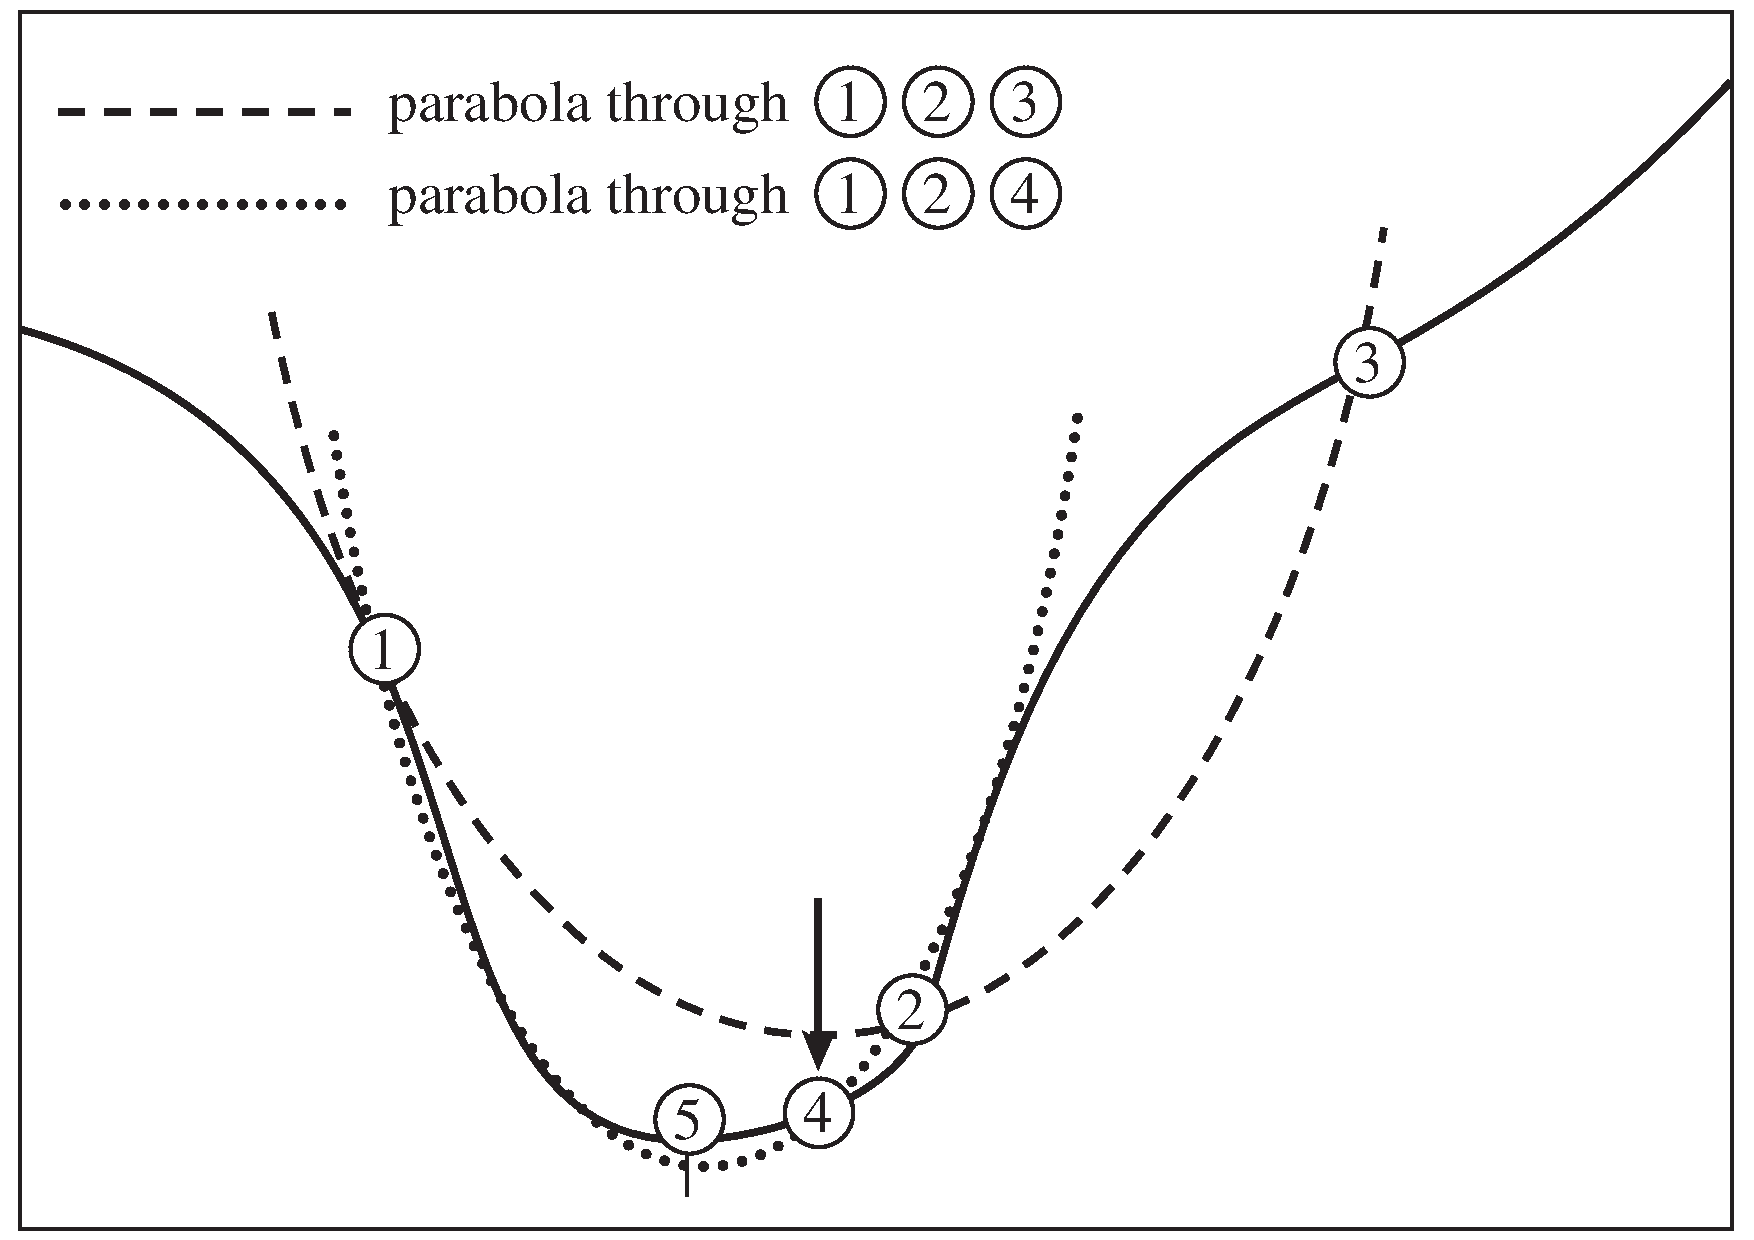
\includegraphics[width=0.55\textwidth]{parabola.pdf}
    \caption{Convergência pelo Método de Brent. Figura retirada de \cite{Brent} }
\label{fig:parabolas}
\end{figure}

A figura \ref{fig:parabolas} mostra duas iterações da interpolação parabólica. É possível notar que a primeira estimativa do minimizador é obtida em $4$ e que, em seguida, esta muda para $5$, se aproximando ainda mais do real valor do minimizador da função $f(x)$.
 
\subsection{Algoritmo}

Durante qualquer fase do algoritmo, este possui um conjunto de 6 pontos $(a, b, u, v, w, x)$. Os pontos $a$ e $b$ definem o intervalo enquadrante de cada iteração; $x$ é o minimizador de $f(x)$ obtido até o momento; $w$ é o ponto de segundo menor valor da função objetivo até o momento e $v$ é o valor anterior de $w$; $u$, por sua vez,  é o ponto onde a função foi avaliada mais recentemente. Um outro ponto que também aparece no algoritmo é o ponto médio entre $a$ e $b$, i.e $x_m$, no entanto, a função objetivo não é avaliada nele.

Se após o passo $d$ da interpolação parabólica, o melhor ponto $x$ pertencer ao intervalo $[a, \, b]$ e, ainda, se o deslocamento provocado por este passo for inferior ao deslocamento provocado na penúltima iteração, significa que $x$ está convergindo e que a interpolação parabólica pode ser usada. Caso alguma dessas condições não seja satisfeita, o passo $d$ é calculado utilizando a razão áurea do maior segmento dentro do intervalo $[a, \,b]$.

\begin{figure}[h!]
\centering
\scalebox{.85}{% Define block styles
\tikzstyle{io} = [trapezium,trapezium left angle=70,trapezium right angle=-70,minimum height=1cm, draw, fill=yellow!20, text width=6em, text badly centered, node distance=2.5cm, inner sep=0pt]
\tikzstyle{decision} = [diamond, draw, fill=red!20, 
    text width=6em, text badly centered, node distance=3cm, inner sep=0pt]
\tikzstyle{block} = [rectangle, draw, fill=blue!20, 
    text width=10em, text centered, rounded corners, minimum height=4em]
    \tikzstyle{block0} = [rectangle, draw, fill=blue!20, 
    text width=4em, text centered, rounded corners, minimum height=4em]
    \tikzstyle{block1} = [rectangle, draw, fill=cyan!20, node distance=3cm,
    text width=5em, text centered, rounded corners, minimum height=4em]
    \tikzstyle{line} = [draw, -latex']
\tikzstyle{cloud} = [draw, ellipse,fill=green!20, node distance=2cm,
    minimum height=2em]
    \tikzstyle{io2} = [trapezium,trapezium left angle=70,trapezium right angle=-70,minimum height=1cm, draw, fill=yellow!20, text width=1.5cm, text badly centered, node distance=3cm, inner sep=0pt]
    
\begin{tikzpicture}[node distance = 2cm, auto]
    % Place nodes
    \node [io] (input) {$I_1 = [a\, b]$\\$\varepsilon: tolerancia$};
    \node [block, below of =input] (init) {Atualiza $x,w,v,u$\\$x_m = \frac{a+b}{2}$}; % $x=w=v$: criterio 3 pontos\\$d_0=0;
    %\node [block, below of = init] (parab) {Atualiza:\\$x$:minimizador parabola\\$w$:segundo menor valor f\\$v$ : $w$ anterior\\$u$: ultima avaliacao $f$\\};
    \node [block, below of =init] (parab) {$r = (x-w)\,(f_x-f_v)$\\$q = (x-v)\,(f_x-f_w)$\\$p = (x-v)\,q - (x-w)\,r$};
    \node [decision, below of=parab] (evaluate) {$(x+d)\in [a\,b]$\\ $\&\&$\\ $d_k<\frac{d_{k-2}}{2}$};
    \node [below of = evaluate](aux){};
    \node [block1,right of = aux,node distance=3cm] (interp) {$d=\frac{p}{q}$};
    \node [block1, left of=aux, node distance=3cm] (gold) {d: Seção Áurea};
    \node [block0, below of=aux] (act) {$u = x + d$};
    \node [decision, below of=act] (evaluate2) {$|x - x_m|<\varepsilon$};
    \node [io2, below of=evaluate2] (out) {$x_{min}=x$};
    \node [cloud,below of = out] (stop) {FIM};
    %\node [left of = parab_step, node distance=3cm](aux2){};
       
    % Draw edges
    \path [line] (input) -- (init);
    \path [line] (init) -- (parab);
    \path [line] (parab) -- (evaluate);
    \path [line,rounded corners] (evaluate.east) -| node [above] {sim} (interp);
    \path [line,rounded corners] (evaluate.west) -| node [above] {não}(gold);
    \path [line,rounded corners] (gold.south) |- (act.west);
    \path [line,rounded corners] (interp.south) |- (act.east);
    \path[line] (act) -- (evaluate2);
    \path [line] (evaluate2) -- node [near start] {sim} (out);
    \path [line,rounded corners] (evaluate2.east)-- ++(35mm,0mm) |- node [above] {não} (init.east);
    \path [line] (out) -- (stop);
\end{tikzpicture}}
\caption{Fluxograma do Método de Interpolação}
\label{fig:brentFlow}
\end{figure}

O algoritmo retoma o início dos cálculos dos novos pontos $(a, b, u, v, w, x)$ até que a tolerância seja atingida ($ |x-x_m| < tol $), alternando,portanto, entre e a interpolação polinomial e o método da razão áurea na determinação dos intervalos para as próximas iterações. O diagrama de fluxo \ref{fig:brentFlow} exemplifica o algoritmo.

\subsection{Resultado}

O resultado obtido para o método de Brent utilizando a função teste apresentada previamente neste relatório (eq. \ref{eq:func_obj}) pode ser observado na figura \ref{fig:brent}.\\

\begin{figure}[h!]
\centering
\scalebox{0.85}{\section{Interpolação Parabólica e o Método de Brent}

\vspace{0.5cm}

\subsection{Princípios básicos}

\vspace{0.5cm}

A idéia por trás desse método é utilizar uma aproximação da função $f(x)$ por um polinômio de grau 2 $g(x)$ que passa por três pontos pertencentes a um intervalo enquadrante. Dessa maneira, aproxima-se o mínimo de $f(x)$ pelo mínimo da parábola obtida. A fórmula \ref{eq:parab} permite encontrar a abcissa $x$ correspondente ao mínimo da parábola para os pontos $a,b$ e $c$.\\

\begin{equation}
  x = b - \frac{1}{2}\frac{(b-a)^2[f(b)-f(c)] - (b-c)^2[f(b)-f(a)]}{(b-a)[f(b)-f(c)] - (b-c)[f(b)-f(a)]} 
  \label{eq:parab}
\end{equation}

\vspace{0.5cm}

Redefine-se, então, o intervalo para a próxima iteração de acordo com a avaliação da função objetivo nesses três pontos, descartando o pior deles e guardando o minimizador desta parábola aproximada como novo ponto. Tal interpolação parabólica é dita inversa pois buscamos a abscissa $x$ e não a ordenada $f(x)$. \\

Da expressão \ref{eq:parab}, podemos notar que existe uma singularidade quando os três pontos são colineares. Além disso, o método funciona da mesma maneira tanto na presença de um mínimo quanto de um máximo. \\

Por isso, para contornar tais dificuldades, a estratégia proposta por Brent é utilizar uma busca segura (ex: seção-áurea) quando que a função for não cooperativa e trocar para para interpolação parabólica inversa sempre que possível. Assim, incorpora-se a robustez do método da seção-áurea com a rapidez da interpolação quadrática.\\

\begin{figure}[!h]
\centering
    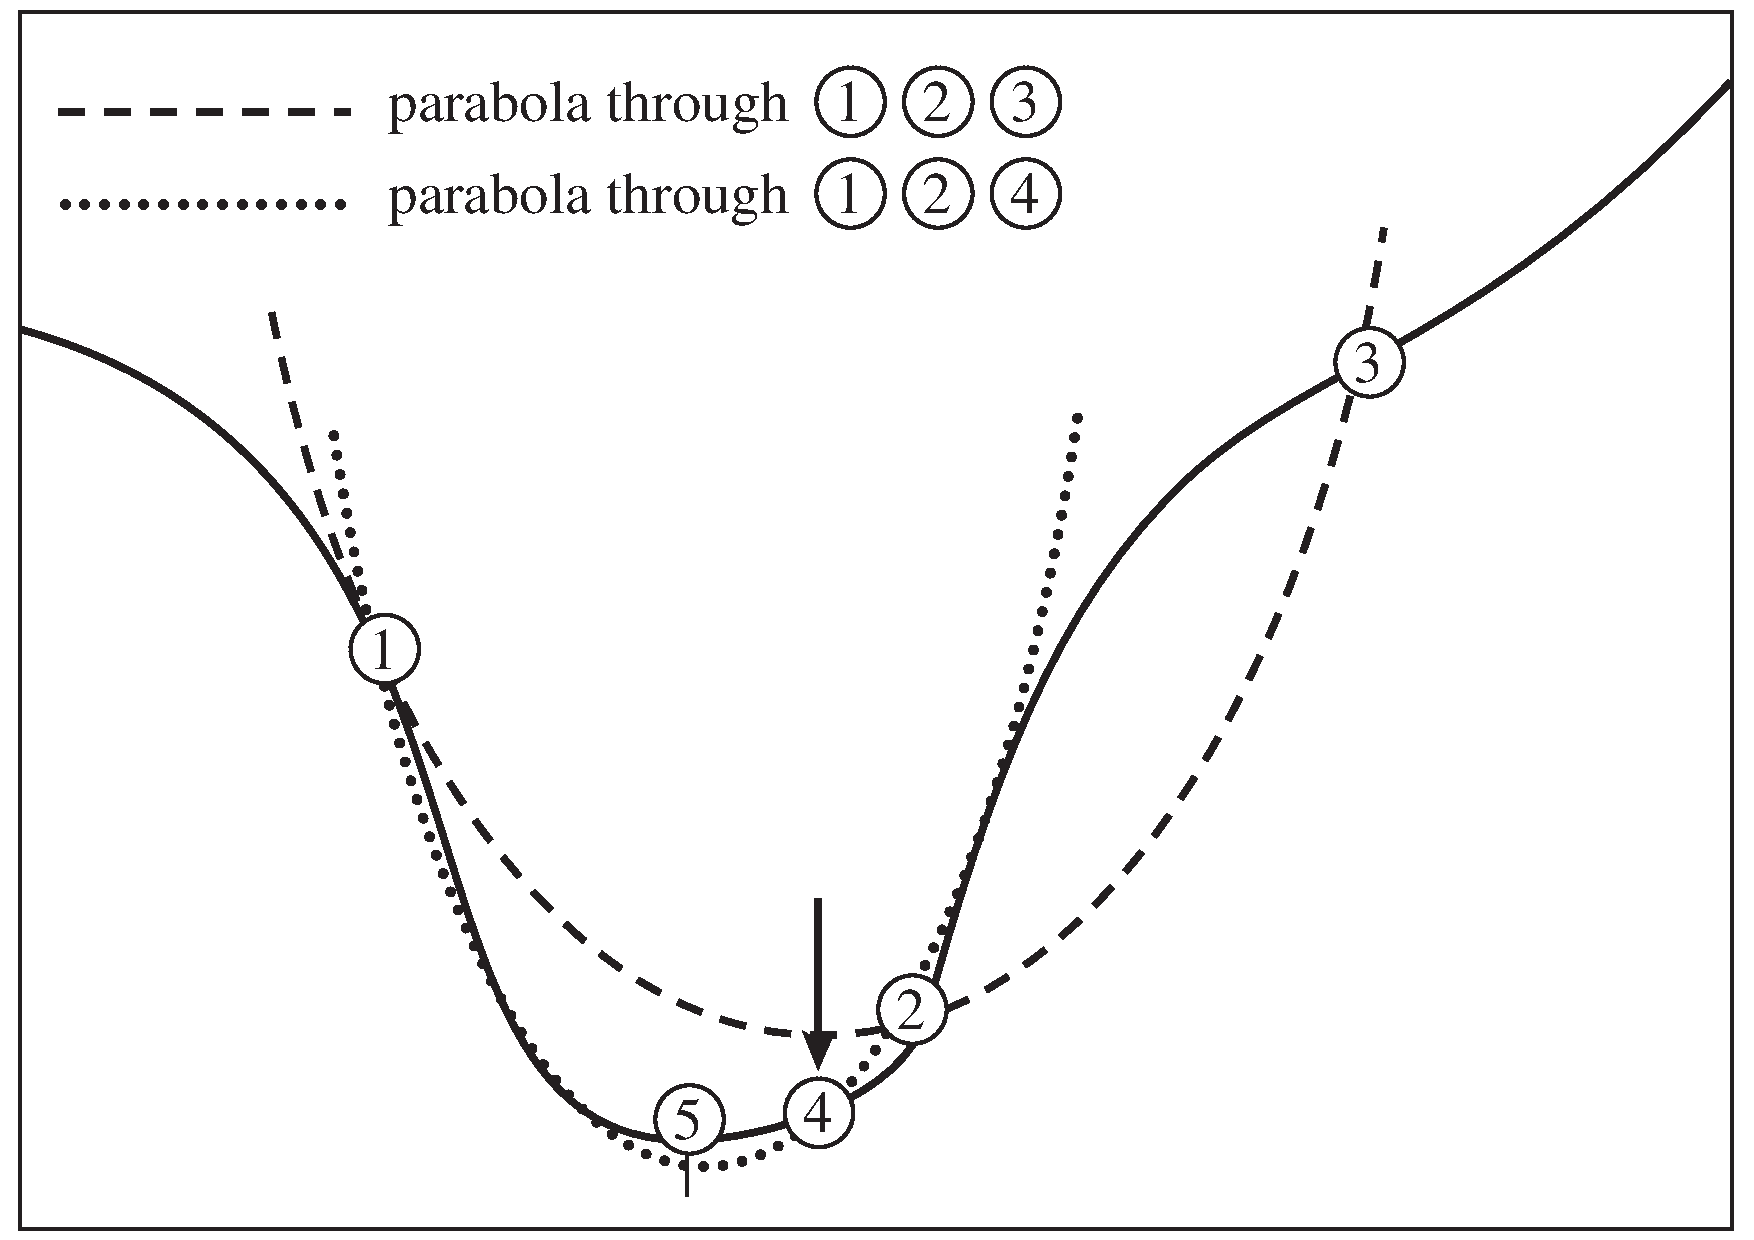
\includegraphics[width=0.75\textwidth]{parabola.pdf}
    \caption{Convergência pelo Método de Brent. Figura retirada de \cite{Brent} }
\label{fig:parabolas}
\end{figure}

A figura \ref{fig:parabolas} mostra duas iterações da interpolação parabólica. É possível notar que a primeira estimativa do minimizador é obtida em $4$ e que, em seguida, esta muda para $5$, se aproximando ainda mais do real valor do minimizador da função $f(x)$.
 
\subsection{Algoritmo}

\vspace{0.5cm}

Durante qualquer fase do algoritmo, este possui um conjunto de 6 pontos $(a, b, u, v, w, x)$. Os pontos $a$ e $b$ definem o intervalo enquadrante de cada iteração; $x$ é o minimizador de $f(x)$ obtido até o momento; $w$ é o ponto de segundo menor valor da função objetivo até o momento e $v$ é o valor anterior de $w$; $u$, por sua vez,  é o ponto onde a função foi avaliada mais recentemente. Um outro ponto que também aparece no algoritmo é o ponto médio entre $a$ e $b$, i.e $x_m$, no entanto, a função objetivo não é avaliada nele.

Se após o passo $d$ da interpolação parabólica, o melhor ponto $x$ pertencer ao intervalo $[a, \, b]$ e, ainda, se o deslocamento provocado por este passo for inferior ao deslocamento provocado na penúltima iteração, significa que $x$ está convergindo e que a interpolação parabólica pode ser usada. Caso alguma dessas condições não seja satisfeita, o passo $d$ é calculado utilizando a razão áurea do maior segmento dentro do intervalo $[a, \,b]$.\\

O algoritmo retoma o início dos cálculos dos novos pontos $(a, b, u, v, w, x)$ até que a tolerância seja atingida ($ |x-x_m| < tol $), alternando,portanto, entre e a interpolação polinomial e o método da razão áurea na determinação dos intervalos para as próximas iterações. O diagrama de fluxo \ref{fig:brentFlow} exemplifica o algoritmo.

 \begin{figure}
 \centering
 \scalebox{1}{% Define block styles
\tikzstyle{io} = [trapezium,trapezium left angle=70,trapezium right angle=-70,minimum height=1cm, draw, fill=yellow!20, text width=6em, text badly centered, node distance=2.5cm, inner sep=0pt]
\tikzstyle{decision} = [diamond, draw, fill=red!20, 
    text width=6em, text badly centered, node distance=3cm, inner sep=0pt]
\tikzstyle{block} = [rectangle, draw, fill=blue!20, 
    text width=10em, text centered, rounded corners, minimum height=4em]
    \tikzstyle{block0} = [rectangle, draw, fill=blue!20, 
    text width=4em, text centered, rounded corners, minimum height=4em]
    \tikzstyle{block1} = [rectangle, draw, fill=cyan!20, node distance=3cm,
    text width=5em, text centered, rounded corners, minimum height=4em]
    \tikzstyle{line} = [draw, -latex']
\tikzstyle{cloud} = [draw, ellipse,fill=green!20, node distance=2cm,
    minimum height=2em]
    \tikzstyle{io2} = [trapezium,trapezium left angle=70,trapezium right angle=-70,minimum height=1cm, draw, fill=yellow!20, text width=1.5cm, text badly centered, node distance=3cm, inner sep=0pt]
    
\begin{tikzpicture}[node distance = 2cm, auto]
    % Place nodes
    \node [io] (input) {$I_1 = [a\, b]$\\$\varepsilon: tolerancia$};
    \node [block, below of =input] (init) {Atualiza $x,w,v,u$\\$x_m = \frac{a+b}{2}$}; % $x=w=v$: criterio 3 pontos\\$d_0=0;
    %\node [block, below of = init] (parab) {Atualiza:\\$x$:minimizador parabola\\$w$:segundo menor valor f\\$v$ : $w$ anterior\\$u$: ultima avaliacao $f$\\};
    \node [block, below of =init] (parab) {$r = (x-w)\,(f_x-f_v)$\\$q = (x-v)\,(f_x-f_w)$\\$p = (x-v)\,q - (x-w)\,r$};
    \node [decision, below of=parab] (evaluate) {$(x+d)\in [a\,b]$\\ $\&\&$\\ $d_k<\frac{d_{k-2}}{2}$};
    \node [below of = evaluate](aux){};
    \node [block1,right of = aux,node distance=3cm] (interp) {$d=\frac{p}{q}$};
    \node [block1, left of=aux, node distance=3cm] (gold) {d: Seção Áurea};
    \node [block0, below of=aux] (act) {$u = x + d$};
    \node [decision, below of=act] (evaluate2) {$|x - x_m|<\varepsilon$};
    \node [io2, below of=evaluate2] (out) {$x_{min}=x$};
    \node [cloud,below of = out] (stop) {FIM};
    %\node [left of = parab_step, node distance=3cm](aux2){};
       
    % Draw edges
    \path [line] (input) -- (init);
    \path [line] (init) -- (parab);
    \path [line] (parab) -- (evaluate);
    \path [line,rounded corners] (evaluate.east) -| node [above] {sim} (interp);
    \path [line,rounded corners] (evaluate.west) -| node [above] {não}(gold);
    \path [line,rounded corners] (gold.south) |- (act.west);
    \path [line,rounded corners] (interp.south) |- (act.east);
    \path[line] (act) -- (evaluate2);
    \path [line] (evaluate2) -- node [near start] {sim} (out);
    \path [line,rounded corners] (evaluate2.east)-- ++(35mm,0mm) |- node [above] {não} (init.east);
    \path [line] (out) -- (stop);
\end{tikzpicture}}
 \caption{Fluxograma do Método de Interpolação}
 \label{fig:brentFlow}
 \end{figure}

\subsection{Resultado}

O resultado obtido para o método de Brent utilizando a função teste apresentada previamente neste relatório (eq. \ref{eq:func_obj}) pode ser observado na figura \ref{fig:brent}.\\

\begin{figure}[h!]
\centering
\scalebox{1}{\section{Interpolação Parabólica e o Método de Brent}

\vspace{0.5cm}

\subsection{Princípios básicos}

\vspace{0.5cm}

A idéia por trás desse método é utilizar uma aproximação da função $f(x)$ por um polinômio de grau 2 $g(x)$ que passa por três pontos pertencentes a um intervalo enquadrante. Dessa maneira, aproxima-se o mínimo de $f(x)$ pelo mínimo da parábola obtida. A fórmula \ref{eq:parab} permite encontrar a abcissa $x$ correspondente ao mínimo da parábola para os pontos $a,b$ e $c$.\\

\begin{equation}
  x = b - \frac{1}{2}\frac{(b-a)^2[f(b)-f(c)] - (b-c)^2[f(b)-f(a)]}{(b-a)[f(b)-f(c)] - (b-c)[f(b)-f(a)]} 
  \label{eq:parab}
\end{equation}

\vspace{0.5cm}

Redefine-se, então, o intervalo para a próxima iteração de acordo com a avaliação da função objetivo nesses três pontos, descartando o pior deles e guardando o minimizador desta parábola aproximada como novo ponto. Tal interpolação parabólica é dita inversa pois buscamos a abscissa $x$ e não a ordenada $f(x)$. \\

Da expressão \ref{eq:parab}, podemos notar que existe uma singularidade quando os três pontos são colineares. Além disso, o método funciona da mesma maneira tanto na presença de um mínimo quanto de um máximo. \\

Por isso, para contornar tais dificuldades, a estratégia proposta por Brent é utilizar uma busca segura (ex: seção-áurea) quando que a função for não cooperativa e trocar para para interpolação parabólica inversa sempre que possível. Assim, incorpora-se a robustez do método da seção-áurea com a rapidez da interpolação quadrática.\\

\begin{figure}[!h]
\centering
    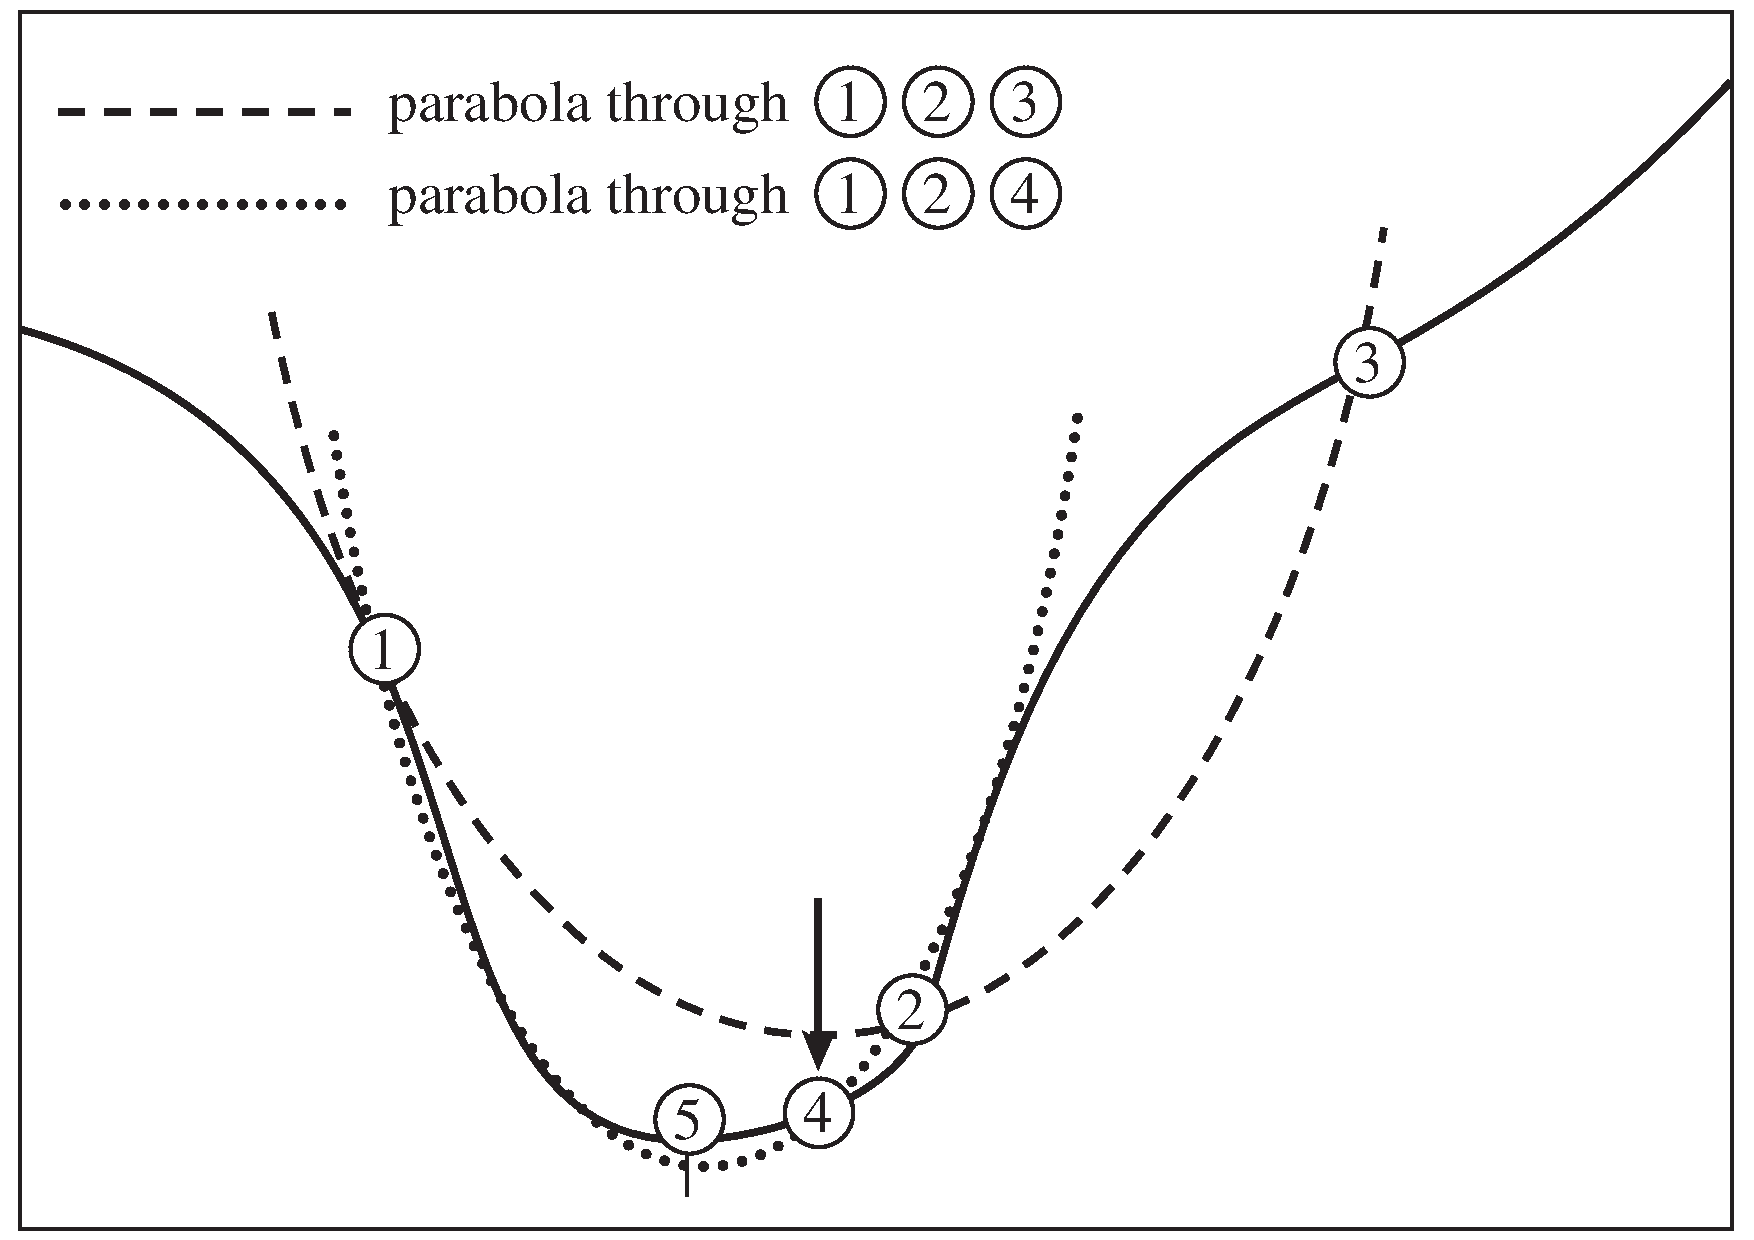
\includegraphics[width=0.75\textwidth]{parabola.pdf}
    \caption{Convergência pelo Método de Brent. Figura retirada de \cite{Brent} }
\label{fig:parabolas}
\end{figure}

A figura \ref{fig:parabolas} mostra duas iterações da interpolação parabólica. É possível notar que a primeira estimativa do minimizador é obtida em $4$ e que, em seguida, esta muda para $5$, se aproximando ainda mais do real valor do minimizador da função $f(x)$.
 
\subsection{Algoritmo}

\vspace{0.5cm}

Durante qualquer fase do algoritmo, este possui um conjunto de 6 pontos $(a, b, u, v, w, x)$. Os pontos $a$ e $b$ definem o intervalo enquadrante de cada iteração; $x$ é o minimizador de $f(x)$ obtido até o momento; $w$ é o ponto de segundo menor valor da função objetivo até o momento e $v$ é o valor anterior de $w$; $u$, por sua vez,  é o ponto onde a função foi avaliada mais recentemente. Um outro ponto que também aparece no algoritmo é o ponto médio entre $a$ e $b$, i.e $x_m$, no entanto, a função objetivo não é avaliada nele.

Se após o passo $d$ da interpolação parabólica, o melhor ponto $x$ pertencer ao intervalo $[a, \, b]$ e, ainda, se o deslocamento provocado por este passo for inferior ao deslocamento provocado na penúltima iteração, significa que $x$ está convergindo e que a interpolação parabólica pode ser usada. Caso alguma dessas condições não seja satisfeita, o passo $d$ é calculado utilizando a razão áurea do maior segmento dentro do intervalo $[a, \,b]$.\\

O algoritmo retoma o início dos cálculos dos novos pontos $(a, b, u, v, w, x)$ até que a tolerância seja atingida ($ |x-x_m| < tol $), alternando,portanto, entre e a interpolação polinomial e o método da razão áurea na determinação dos intervalos para as próximas iterações. O diagrama de fluxo \ref{fig:brentFlow} exemplifica o algoritmo.

 \begin{figure}
 \centering
 \scalebox{1}{% Define block styles
\tikzstyle{io} = [trapezium,trapezium left angle=70,trapezium right angle=-70,minimum height=1cm, draw, fill=yellow!20, text width=6em, text badly centered, node distance=2.5cm, inner sep=0pt]
\tikzstyle{decision} = [diamond, draw, fill=red!20, 
    text width=6em, text badly centered, node distance=3cm, inner sep=0pt]
\tikzstyle{block} = [rectangle, draw, fill=blue!20, 
    text width=10em, text centered, rounded corners, minimum height=4em]
    \tikzstyle{block0} = [rectangle, draw, fill=blue!20, 
    text width=4em, text centered, rounded corners, minimum height=4em]
    \tikzstyle{block1} = [rectangle, draw, fill=cyan!20, node distance=3cm,
    text width=5em, text centered, rounded corners, minimum height=4em]
    \tikzstyle{line} = [draw, -latex']
\tikzstyle{cloud} = [draw, ellipse,fill=green!20, node distance=2cm,
    minimum height=2em]
    \tikzstyle{io2} = [trapezium,trapezium left angle=70,trapezium right angle=-70,minimum height=1cm, draw, fill=yellow!20, text width=1.5cm, text badly centered, node distance=3cm, inner sep=0pt]
    
\begin{tikzpicture}[node distance = 2cm, auto]
    % Place nodes
    \node [io] (input) {$I_1 = [a\, b]$\\$\varepsilon: tolerancia$};
    \node [block, below of =input] (init) {Atualiza $x,w,v,u$\\$x_m = \frac{a+b}{2}$}; % $x=w=v$: criterio 3 pontos\\$d_0=0;
    %\node [block, below of = init] (parab) {Atualiza:\\$x$:minimizador parabola\\$w$:segundo menor valor f\\$v$ : $w$ anterior\\$u$: ultima avaliacao $f$\\};
    \node [block, below of =init] (parab) {$r = (x-w)\,(f_x-f_v)$\\$q = (x-v)\,(f_x-f_w)$\\$p = (x-v)\,q - (x-w)\,r$};
    \node [decision, below of=parab] (evaluate) {$(x+d)\in [a\,b]$\\ $\&\&$\\ $d_k<\frac{d_{k-2}}{2}$};
    \node [below of = evaluate](aux){};
    \node [block1,right of = aux,node distance=3cm] (interp) {$d=\frac{p}{q}$};
    \node [block1, left of=aux, node distance=3cm] (gold) {d: Seção Áurea};
    \node [block0, below of=aux] (act) {$u = x + d$};
    \node [decision, below of=act] (evaluate2) {$|x - x_m|<\varepsilon$};
    \node [io2, below of=evaluate2] (out) {$x_{min}=x$};
    \node [cloud,below of = out] (stop) {FIM};
    %\node [left of = parab_step, node distance=3cm](aux2){};
       
    % Draw edges
    \path [line] (input) -- (init);
    \path [line] (init) -- (parab);
    \path [line] (parab) -- (evaluate);
    \path [line,rounded corners] (evaluate.east) -| node [above] {sim} (interp);
    \path [line,rounded corners] (evaluate.west) -| node [above] {não}(gold);
    \path [line,rounded corners] (gold.south) |- (act.west);
    \path [line,rounded corners] (interp.south) |- (act.east);
    \path[line] (act) -- (evaluate2);
    \path [line] (evaluate2) -- node [near start] {sim} (out);
    \path [line,rounded corners] (evaluate2.east)-- ++(35mm,0mm) |- node [above] {não} (init.east);
    \path [line] (out) -- (stop);
\end{tikzpicture}}
 \caption{Fluxograma do Método de Interpolação}
 \label{fig:brentFlow}
 \end{figure}

\subsection{Resultado}

O resultado obtido para o método de Brent utilizando a função teste apresentada previamente neste relatório (eq. \ref{eq:func_obj}) pode ser observado na figura \ref{fig:brent}.\\

\begin{figure}[h!]
\centering
\scalebox{1}{\section{Interpolação Parabólica e o Método de Brent}

\vspace{0.5cm}

\subsection{Princípios básicos}

\vspace{0.5cm}

A idéia por trás desse método é utilizar uma aproximação da função $f(x)$ por um polinômio de grau 2 $g(x)$ que passa por três pontos pertencentes a um intervalo enquadrante. Dessa maneira, aproxima-se o mínimo de $f(x)$ pelo mínimo da parábola obtida. A fórmula \ref{eq:parab} permite encontrar a abcissa $x$ correspondente ao mínimo da parábola para os pontos $a,b$ e $c$.\\

\begin{equation}
  x = b - \frac{1}{2}\frac{(b-a)^2[f(b)-f(c)] - (b-c)^2[f(b)-f(a)]}{(b-a)[f(b)-f(c)] - (b-c)[f(b)-f(a)]} 
  \label{eq:parab}
\end{equation}

\vspace{0.5cm}

Redefine-se, então, o intervalo para a próxima iteração de acordo com a avaliação da função objetivo nesses três pontos, descartando o pior deles e guardando o minimizador desta parábola aproximada como novo ponto. Tal interpolação parabólica é dita inversa pois buscamos a abscissa $x$ e não a ordenada $f(x)$. \\

Da expressão \ref{eq:parab}, podemos notar que existe uma singularidade quando os três pontos são colineares. Além disso, o método funciona da mesma maneira tanto na presença de um mínimo quanto de um máximo. \\

Por isso, para contornar tais dificuldades, a estratégia proposta por Brent é utilizar uma busca segura (ex: seção-áurea) quando que a função for não cooperativa e trocar para para interpolação parabólica inversa sempre que possível. Assim, incorpora-se a robustez do método da seção-áurea com a rapidez da interpolação quadrática.\\

\begin{figure}[!h]
\centering
    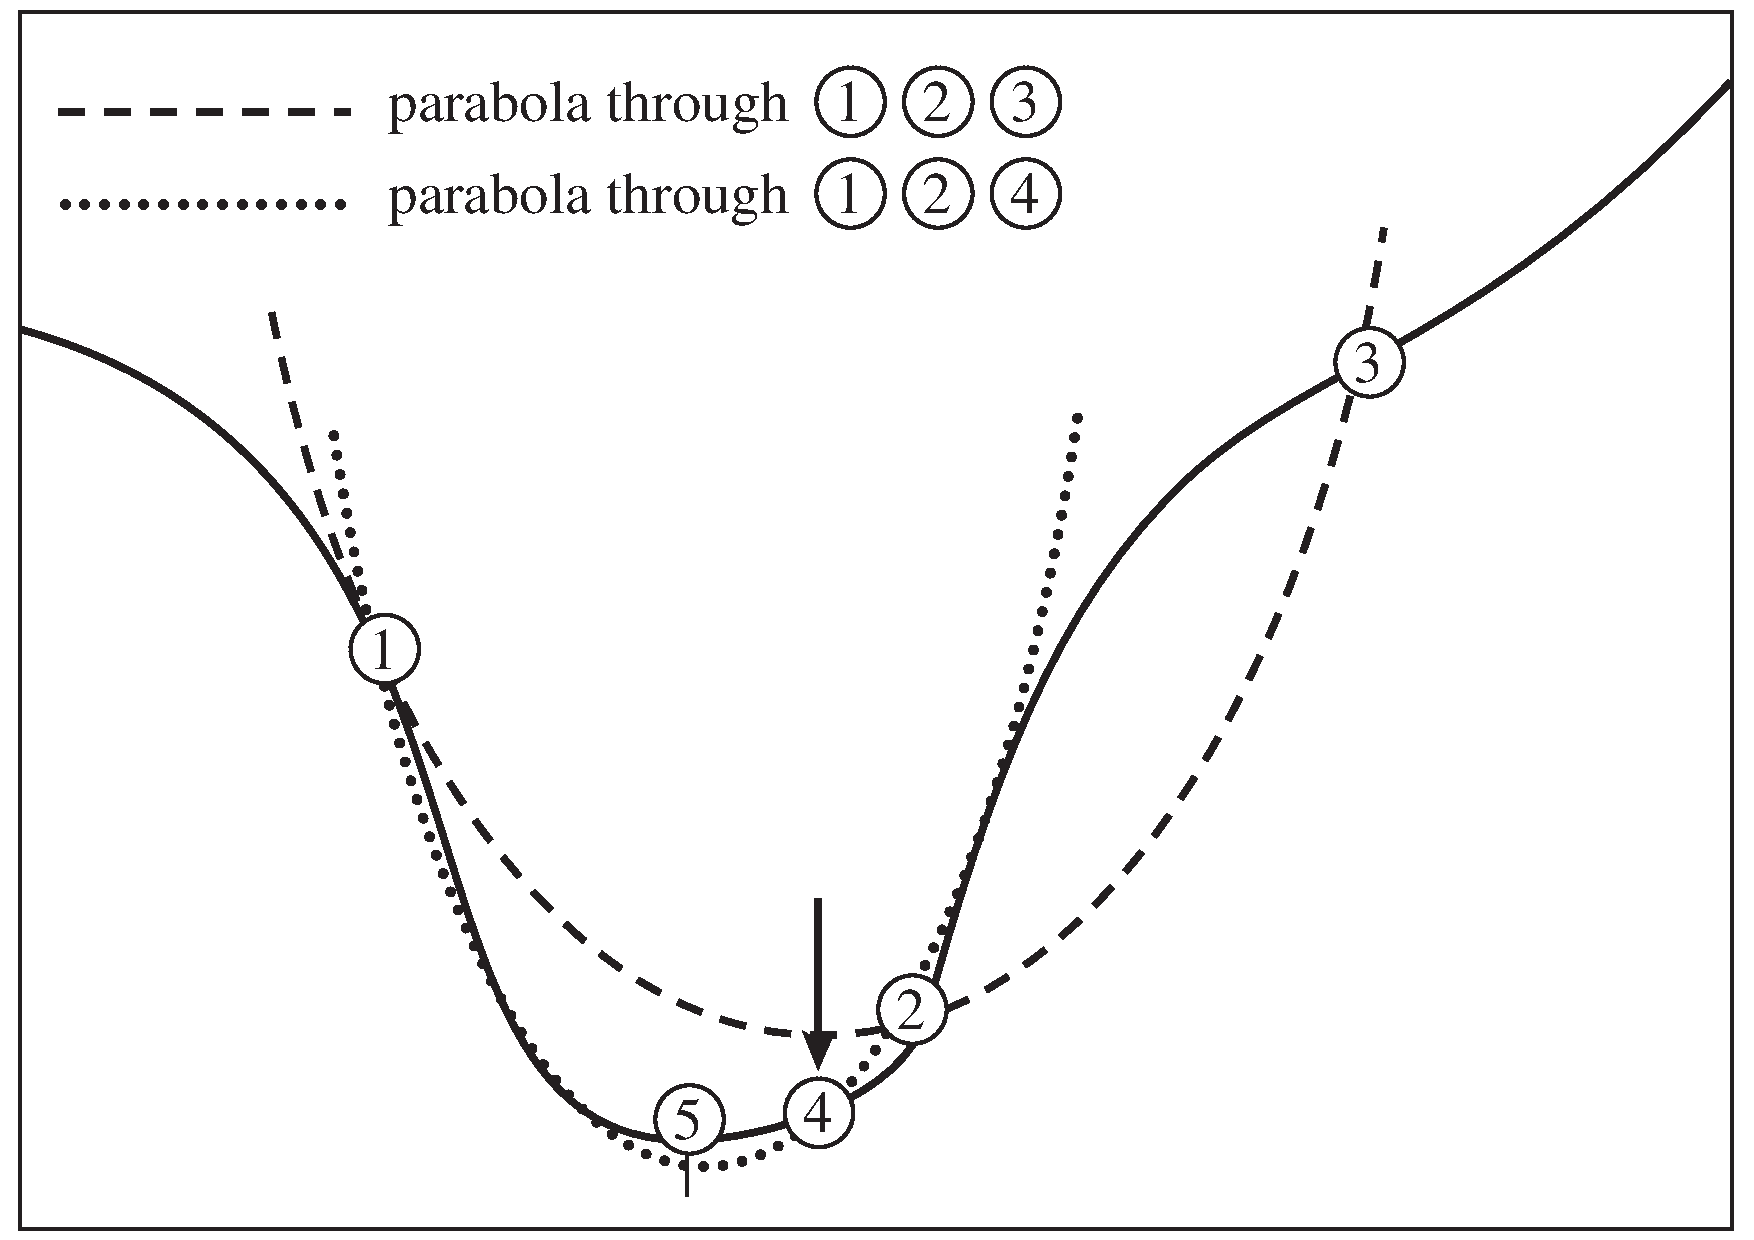
\includegraphics[width=0.75\textwidth]{parabola.pdf}
    \caption{Convergência pelo Método de Brent. Figura retirada de \cite{Brent} }
\label{fig:parabolas}
\end{figure}

A figura \ref{fig:parabolas} mostra duas iterações da interpolação parabólica. É possível notar que a primeira estimativa do minimizador é obtida em $4$ e que, em seguida, esta muda para $5$, se aproximando ainda mais do real valor do minimizador da função $f(x)$.
 
\subsection{Algoritmo}

\vspace{0.5cm}

Durante qualquer fase do algoritmo, este possui um conjunto de 6 pontos $(a, b, u, v, w, x)$. Os pontos $a$ e $b$ definem o intervalo enquadrante de cada iteração; $x$ é o minimizador de $f(x)$ obtido até o momento; $w$ é o ponto de segundo menor valor da função objetivo até o momento e $v$ é o valor anterior de $w$; $u$, por sua vez,  é o ponto onde a função foi avaliada mais recentemente. Um outro ponto que também aparece no algoritmo é o ponto médio entre $a$ e $b$, i.e $x_m$, no entanto, a função objetivo não é avaliada nele.

Se após o passo $d$ da interpolação parabólica, o melhor ponto $x$ pertencer ao intervalo $[a, \, b]$ e, ainda, se o deslocamento provocado por este passo for inferior ao deslocamento provocado na penúltima iteração, significa que $x$ está convergindo e que a interpolação parabólica pode ser usada. Caso alguma dessas condições não seja satisfeita, o passo $d$ é calculado utilizando a razão áurea do maior segmento dentro do intervalo $[a, \,b]$.\\

O algoritmo retoma o início dos cálculos dos novos pontos $(a, b, u, v, w, x)$ até que a tolerância seja atingida ($ |x-x_m| < tol $), alternando,portanto, entre e a interpolação polinomial e o método da razão áurea na determinação dos intervalos para as próximas iterações. O diagrama de fluxo \ref{fig:brentFlow} exemplifica o algoritmo.

 \begin{figure}
 \centering
 \scalebox{1}{\input{brentFlow.tex}}
 \caption{Fluxograma do Método de Interpolação}
 \label{fig:brentFlow}
 \end{figure}

\subsection{Resultado}

O resultado obtido para o método de Brent utilizando a função teste apresentada previamente neste relatório (eq. \ref{eq:func_obj}) pode ser observado na figura \ref{fig:brent}.\\

\begin{figure}[h!]
\centering
\scalebox{1}{\input{./figuras/brent.tex}}
\caption{Tolerância: $\epsilon =  0.01$. Número de iterações: $n = 12$}
\label{fig:brent}
\end{figure}

É interessante notar que a performance foi bem similar ao método da seção áurea já que a tolerância $\epsilon$ escolhida foi a mesma. No entanto, o método de Brent é consideravelmente mais rápido devido à utilizão da interpolação polinomial. Ao passo que foram necessárias 17 iterações para Seção Áurea convergir, somente 12 bastaram para garantir o mesmo resultado usando o método de Brent.}
\caption{Tolerância: $\epsilon =  0.01$. Número de iterações: $n = 12$}
\label{fig:brent}
\end{figure}

É interessante notar que a performance foi bem similar ao método da seção áurea já que a tolerância $\epsilon$ escolhida foi a mesma. No entanto, o método de Brent é consideravelmente mais rápido devido à utilizão da interpolação polinomial. Ao passo que foram necessárias 17 iterações para Seção Áurea convergir, somente 12 bastaram para garantir o mesmo resultado usando o método de Brent.}
\caption{Tolerância: $\epsilon =  0.01$. Número de iterações: $n = 12$}
\label{fig:brent}
\end{figure}

É interessante notar que a performance foi bem similar ao método da seção áurea já que a tolerância $\epsilon$ escolhida foi a mesma. No entanto, o método de Brent é consideravelmente mais rápido devido à utilizão da interpolação polinomial. Ao passo que foram necessárias 17 iterações para Seção Áurea convergir, somente 12 bastaram para garantir o mesmo resultado usando o método de Brent.}
\caption{Tolerância: $\epsilon =  0.01$. Número de iterações: $n = 12$}
\label{fig:brent}
\end{figure}

É interessante notar que a performance foi bem similar ao método da seção áurea já que a tolerância $\epsilon$ escolhida foi a mesma. No entanto, o método de Brent é consideravelmente mais rápido devido à utilizão da interpolação polinomial. Ao passo que foram necessárias 17 iterações para Seção Áurea convergir, somente 12 bastaram para garantir o mesmo resultado usando o método de Brent.

% \section{Interpolação Parabólica e o Método de Brent}

\vspace{0.5cm}

\subsection{Princípios básicos}

\vspace{0.5cm}

A idéia por trás desse método é utilizar uma aproximação da função $f(x)$ por um polinômio de grau 2 $g(x)$ que passa por três pontos pertencentes a um intervalo enquadrante. Dessa maneira, aproxima-se o mínimo de $f(x)$ pelo mínimo da parábola obtida. A fórmula \ref{eq:parab} permite encontrar a abcissa $x$ correspondente ao mínimo da parábola para os pontos $a,b$ e $c$.\\

\begin{equation}
  x = b - \frac{1}{2}\frac{(b-a)^2[f(b)-f(c)] - (b-c)^2[f(b)-f(a)]}{(b-a)[f(b)-f(c)] - (b-c)[f(b)-f(a)]} 
  \label{eq:parab}
\end{equation}

\vspace{0.5cm}

Redefine-se, então, o intervalo para a próxima iteração de acordo com a avaliação da função objetivo nesses três pontos, descartando o pior deles e guardando o minimizador desta parábola aproximada como novo ponto. Tal interpolação parabólica é dita inversa pois buscamos a abscissa $x$ e não a ordenada $f(x)$. \\

Da expressão \ref{eq:parab}, podemos notar que existe uma singularidade quando os três pontos são colineares. Além disso, o método funciona da mesma maneira tanto na presença de um mínimo quanto de um máximo. \\

Por isso, para contornar tais dificuldades, a estratégia proposta por Brent é utilizar uma busca segura (ex: seção-áurea) quando que a função for não cooperativa e trocar para para interpolação parabólica inversa sempre que possível. Assim, incorpora-se a robustez do método da seção-áurea com a rapidez da interpolação quadrática.\\

\begin{figure}[!h]
\centering
    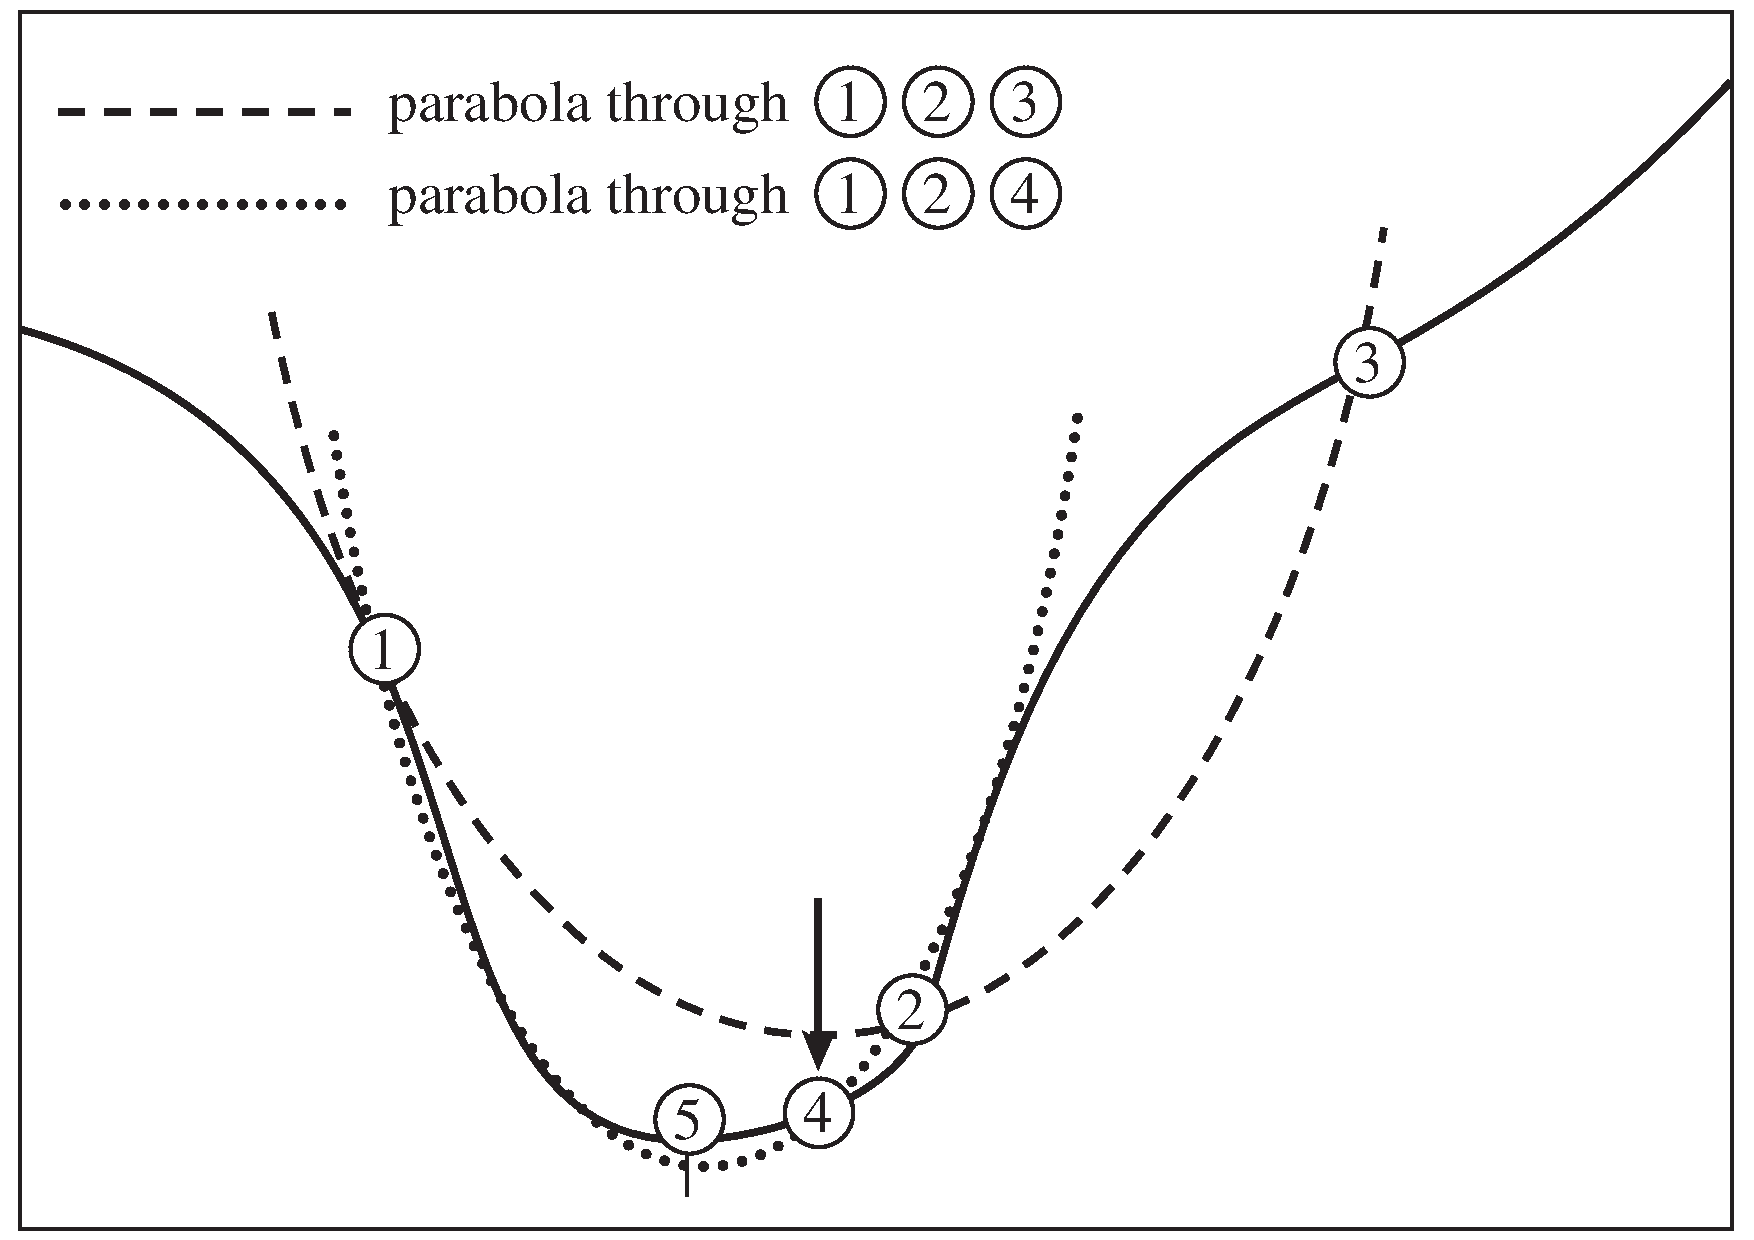
\includegraphics[width=0.75\textwidth]{parabola.pdf}
    \caption{Convergência pelo Método de Brent. Figura retirada de \cite{Brent} }
\label{fig:parabolas}
\end{figure}

A figura \ref{fig:parabolas} mostra duas iterações da interpolação parabólica. É possível notar que a primeira estimativa do minimizador é obtida em $4$ e que, em seguida, esta muda para $5$, se aproximando ainda mais do real valor do minimizador da função $f(x)$.
 
\subsection{Algoritmo}

\vspace{0.5cm}

Durante qualquer fase do algoritmo, este possui um conjunto de 6 pontos $(a, b, u, v, w, x)$. Os pontos $a$ e $b$ definem o intervalo enquadrante de cada iteração; $x$ é o minimizador de $f(x)$ obtido até o momento; $w$ é o ponto de segundo menor valor da função objetivo até o momento e $v$ é o valor anterior de $w$; $u$, por sua vez,  é o ponto onde a função foi avaliada mais recentemente. Um outro ponto que também aparece no algoritmo é o ponto médio entre $a$ e $b$, i.e $x_m$, no entanto, a função objetivo não é avaliada nele.

Se após o passo $d$ da interpolação parabólica, o melhor ponto $x$ pertencer ao intervalo $[a, \, b]$ e, ainda, se o deslocamento provocado por este passo for inferior ao deslocamento provocado na penúltima iteração, significa que $x$ está convergindo e que a interpolação parabólica pode ser usada. Caso alguma dessas condições não seja satisfeita, o passo $d$ é calculado utilizando a razão áurea do maior segmento dentro do intervalo $[a, \,b]$.\\

O algoritmo retoma o início dos cálculos dos novos pontos $(a, b, u, v, w, x)$ até que a tolerância seja atingida ($ |x-x_m| < tol $), alternando,portanto, entre e a interpolação polinomial e o método da razão áurea na determinação dos intervalos para as próximas iterações. O diagrama de fluxo \ref{fig:brentFlow} exemplifica o algoritmo.

 \begin{figure}
 \centering
 \scalebox{1}{% Define block styles
\tikzstyle{io} = [trapezium,trapezium left angle=70,trapezium right angle=-70,minimum height=1cm, draw, fill=yellow!20, text width=6em, text badly centered, node distance=2.5cm, inner sep=0pt]
\tikzstyle{decision} = [diamond, draw, fill=red!20, 
    text width=6em, text badly centered, node distance=3cm, inner sep=0pt]
\tikzstyle{block} = [rectangle, draw, fill=blue!20, 
    text width=10em, text centered, rounded corners, minimum height=4em]
    \tikzstyle{block0} = [rectangle, draw, fill=blue!20, 
    text width=4em, text centered, rounded corners, minimum height=4em]
    \tikzstyle{block1} = [rectangle, draw, fill=cyan!20, node distance=3cm,
    text width=5em, text centered, rounded corners, minimum height=4em]
    \tikzstyle{line} = [draw, -latex']
\tikzstyle{cloud} = [draw, ellipse,fill=green!20, node distance=2cm,
    minimum height=2em]
    \tikzstyle{io2} = [trapezium,trapezium left angle=70,trapezium right angle=-70,minimum height=1cm, draw, fill=yellow!20, text width=1.5cm, text badly centered, node distance=3cm, inner sep=0pt]
    
\begin{tikzpicture}[node distance = 2cm, auto]
    % Place nodes
    \node [io] (input) {$I_1 = [a\, b]$\\$\varepsilon: tolerancia$};
    \node [block, below of =input] (init) {Atualiza $x,w,v,u$\\$x_m = \frac{a+b}{2}$}; % $x=w=v$: criterio 3 pontos\\$d_0=0;
    %\node [block, below of = init] (parab) {Atualiza:\\$x$:minimizador parabola\\$w$:segundo menor valor f\\$v$ : $w$ anterior\\$u$: ultima avaliacao $f$\\};
    \node [block, below of =init] (parab) {$r = (x-w)\,(f_x-f_v)$\\$q = (x-v)\,(f_x-f_w)$\\$p = (x-v)\,q - (x-w)\,r$};
    \node [decision, below of=parab] (evaluate) {$(x+d)\in [a\,b]$\\ $\&\&$\\ $d_k<\frac{d_{k-2}}{2}$};
    \node [below of = evaluate](aux){};
    \node [block1,right of = aux,node distance=3cm] (interp) {$d=\frac{p}{q}$};
    \node [block1, left of=aux, node distance=3cm] (gold) {d: Seção Áurea};
    \node [block0, below of=aux] (act) {$u = x + d$};
    \node [decision, below of=act] (evaluate2) {$|x - x_m|<\varepsilon$};
    \node [io2, below of=evaluate2] (out) {$x_{min}=x$};
    \node [cloud,below of = out] (stop) {FIM};
    %\node [left of = parab_step, node distance=3cm](aux2){};
       
    % Draw edges
    \path [line] (input) -- (init);
    \path [line] (init) -- (parab);
    \path [line] (parab) -- (evaluate);
    \path [line,rounded corners] (evaluate.east) -| node [above] {sim} (interp);
    \path [line,rounded corners] (evaluate.west) -| node [above] {não}(gold);
    \path [line,rounded corners] (gold.south) |- (act.west);
    \path [line,rounded corners] (interp.south) |- (act.east);
    \path[line] (act) -- (evaluate2);
    \path [line] (evaluate2) -- node [near start] {sim} (out);
    \path [line,rounded corners] (evaluate2.east)-- ++(35mm,0mm) |- node [above] {não} (init.east);
    \path [line] (out) -- (stop);
\end{tikzpicture}}
 \caption{Fluxograma do Método de Interpolação}
 \label{fig:brentFlow}
 \end{figure}

\subsection{Resultado}

O resultado obtido para o método de Brent utilizando a função teste apresentada previamente neste relatório (eq. \ref{eq:func_obj}) pode ser observado na figura \ref{fig:brent}.\\

\begin{figure}[h!]
\centering
\scalebox{1}{\section{Interpolação Parabólica e o Método de Brent}

\vspace{0.5cm}

\subsection{Princípios básicos}

\vspace{0.5cm}

A idéia por trás desse método é utilizar uma aproximação da função $f(x)$ por um polinômio de grau 2 $g(x)$ que passa por três pontos pertencentes a um intervalo enquadrante. Dessa maneira, aproxima-se o mínimo de $f(x)$ pelo mínimo da parábola obtida. A fórmula \ref{eq:parab} permite encontrar a abcissa $x$ correspondente ao mínimo da parábola para os pontos $a,b$ e $c$.\\

\begin{equation}
  x = b - \frac{1}{2}\frac{(b-a)^2[f(b)-f(c)] - (b-c)^2[f(b)-f(a)]}{(b-a)[f(b)-f(c)] - (b-c)[f(b)-f(a)]} 
  \label{eq:parab}
\end{equation}

\vspace{0.5cm}

Redefine-se, então, o intervalo para a próxima iteração de acordo com a avaliação da função objetivo nesses três pontos, descartando o pior deles e guardando o minimizador desta parábola aproximada como novo ponto. Tal interpolação parabólica é dita inversa pois buscamos a abscissa $x$ e não a ordenada $f(x)$. \\

Da expressão \ref{eq:parab}, podemos notar que existe uma singularidade quando os três pontos são colineares. Além disso, o método funciona da mesma maneira tanto na presença de um mínimo quanto de um máximo. \\

Por isso, para contornar tais dificuldades, a estratégia proposta por Brent é utilizar uma busca segura (ex: seção-áurea) quando que a função for não cooperativa e trocar para para interpolação parabólica inversa sempre que possível. Assim, incorpora-se a robustez do método da seção-áurea com a rapidez da interpolação quadrática.\\

\begin{figure}[!h]
\centering
    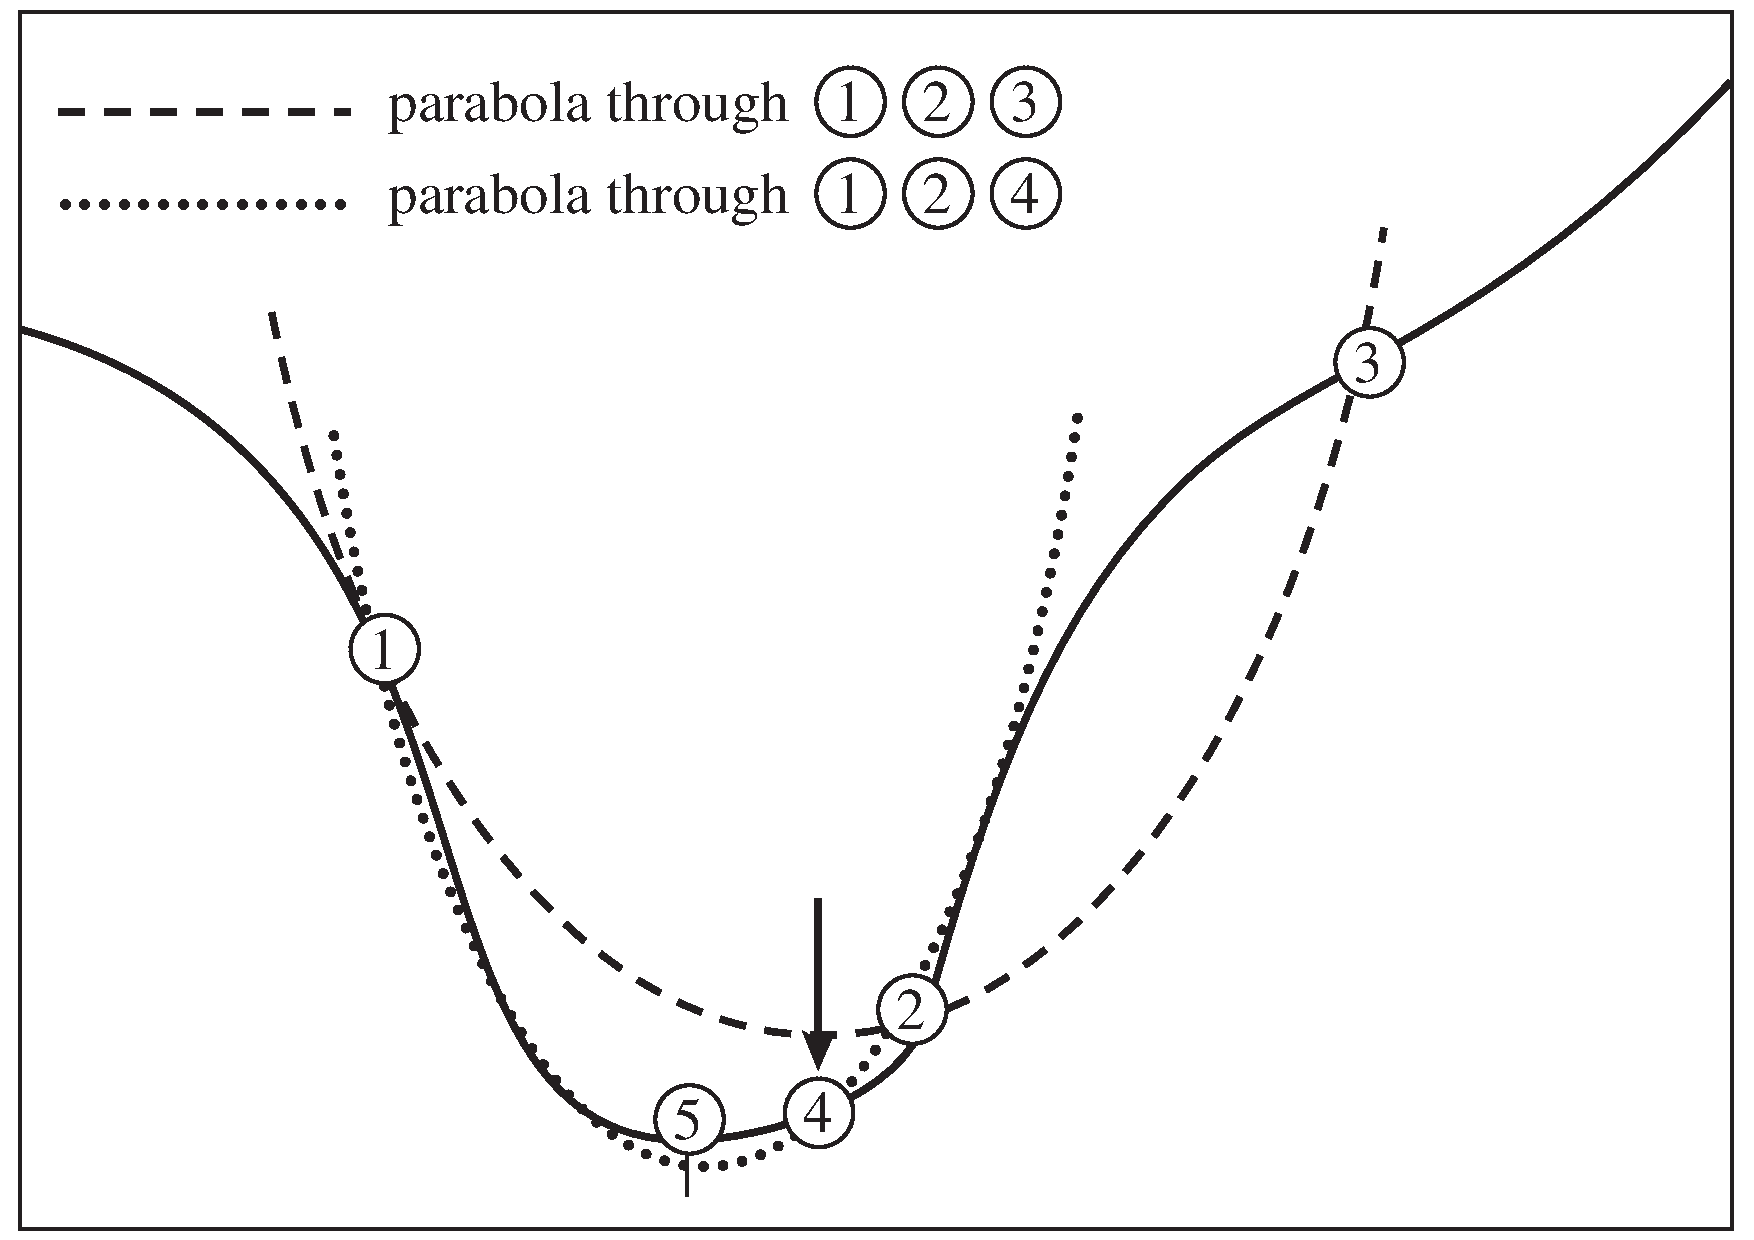
\includegraphics[width=0.75\textwidth]{parabola.pdf}
    \caption{Convergência pelo Método de Brent. Figura retirada de \cite{Brent} }
\label{fig:parabolas}
\end{figure}

A figura \ref{fig:parabolas} mostra duas iterações da interpolação parabólica. É possível notar que a primeira estimativa do minimizador é obtida em $4$ e que, em seguida, esta muda para $5$, se aproximando ainda mais do real valor do minimizador da função $f(x)$.
 
\subsection{Algoritmo}

\vspace{0.5cm}

Durante qualquer fase do algoritmo, este possui um conjunto de 6 pontos $(a, b, u, v, w, x)$. Os pontos $a$ e $b$ definem o intervalo enquadrante de cada iteração; $x$ é o minimizador de $f(x)$ obtido até o momento; $w$ é o ponto de segundo menor valor da função objetivo até o momento e $v$ é o valor anterior de $w$; $u$, por sua vez,  é o ponto onde a função foi avaliada mais recentemente. Um outro ponto que também aparece no algoritmo é o ponto médio entre $a$ e $b$, i.e $x_m$, no entanto, a função objetivo não é avaliada nele.

Se após o passo $d$ da interpolação parabólica, o melhor ponto $x$ pertencer ao intervalo $[a, \, b]$ e, ainda, se o deslocamento provocado por este passo for inferior ao deslocamento provocado na penúltima iteração, significa que $x$ está convergindo e que a interpolação parabólica pode ser usada. Caso alguma dessas condições não seja satisfeita, o passo $d$ é calculado utilizando a razão áurea do maior segmento dentro do intervalo $[a, \,b]$.\\

O algoritmo retoma o início dos cálculos dos novos pontos $(a, b, u, v, w, x)$ até que a tolerância seja atingida ($ |x-x_m| < tol $), alternando,portanto, entre e a interpolação polinomial e o método da razão áurea na determinação dos intervalos para as próximas iterações. O diagrama de fluxo \ref{fig:brentFlow} exemplifica o algoritmo.

 \begin{figure}
 \centering
 \scalebox{1}{% Define block styles
\tikzstyle{io} = [trapezium,trapezium left angle=70,trapezium right angle=-70,minimum height=1cm, draw, fill=yellow!20, text width=6em, text badly centered, node distance=2.5cm, inner sep=0pt]
\tikzstyle{decision} = [diamond, draw, fill=red!20, 
    text width=6em, text badly centered, node distance=3cm, inner sep=0pt]
\tikzstyle{block} = [rectangle, draw, fill=blue!20, 
    text width=10em, text centered, rounded corners, minimum height=4em]
    \tikzstyle{block0} = [rectangle, draw, fill=blue!20, 
    text width=4em, text centered, rounded corners, minimum height=4em]
    \tikzstyle{block1} = [rectangle, draw, fill=cyan!20, node distance=3cm,
    text width=5em, text centered, rounded corners, minimum height=4em]
    \tikzstyle{line} = [draw, -latex']
\tikzstyle{cloud} = [draw, ellipse,fill=green!20, node distance=2cm,
    minimum height=2em]
    \tikzstyle{io2} = [trapezium,trapezium left angle=70,trapezium right angle=-70,minimum height=1cm, draw, fill=yellow!20, text width=1.5cm, text badly centered, node distance=3cm, inner sep=0pt]
    
\begin{tikzpicture}[node distance = 2cm, auto]
    % Place nodes
    \node [io] (input) {$I_1 = [a\, b]$\\$\varepsilon: tolerancia$};
    \node [block, below of =input] (init) {Atualiza $x,w,v,u$\\$x_m = \frac{a+b}{2}$}; % $x=w=v$: criterio 3 pontos\\$d_0=0;
    %\node [block, below of = init] (parab) {Atualiza:\\$x$:minimizador parabola\\$w$:segundo menor valor f\\$v$ : $w$ anterior\\$u$: ultima avaliacao $f$\\};
    \node [block, below of =init] (parab) {$r = (x-w)\,(f_x-f_v)$\\$q = (x-v)\,(f_x-f_w)$\\$p = (x-v)\,q - (x-w)\,r$};
    \node [decision, below of=parab] (evaluate) {$(x+d)\in [a\,b]$\\ $\&\&$\\ $d_k<\frac{d_{k-2}}{2}$};
    \node [below of = evaluate](aux){};
    \node [block1,right of = aux,node distance=3cm] (interp) {$d=\frac{p}{q}$};
    \node [block1, left of=aux, node distance=3cm] (gold) {d: Seção Áurea};
    \node [block0, below of=aux] (act) {$u = x + d$};
    \node [decision, below of=act] (evaluate2) {$|x - x_m|<\varepsilon$};
    \node [io2, below of=evaluate2] (out) {$x_{min}=x$};
    \node [cloud,below of = out] (stop) {FIM};
    %\node [left of = parab_step, node distance=3cm](aux2){};
       
    % Draw edges
    \path [line] (input) -- (init);
    \path [line] (init) -- (parab);
    \path [line] (parab) -- (evaluate);
    \path [line,rounded corners] (evaluate.east) -| node [above] {sim} (interp);
    \path [line,rounded corners] (evaluate.west) -| node [above] {não}(gold);
    \path [line,rounded corners] (gold.south) |- (act.west);
    \path [line,rounded corners] (interp.south) |- (act.east);
    \path[line] (act) -- (evaluate2);
    \path [line] (evaluate2) -- node [near start] {sim} (out);
    \path [line,rounded corners] (evaluate2.east)-- ++(35mm,0mm) |- node [above] {não} (init.east);
    \path [line] (out) -- (stop);
\end{tikzpicture}}
 \caption{Fluxograma do Método de Interpolação}
 \label{fig:brentFlow}
 \end{figure}

\subsection{Resultado}

O resultado obtido para o método de Brent utilizando a função teste apresentada previamente neste relatório (eq. \ref{eq:func_obj}) pode ser observado na figura \ref{fig:brent}.\\

\begin{figure}[h!]
\centering
\scalebox{1}{\section{Interpolação Parabólica e o Método de Brent}

\vspace{0.5cm}

\subsection{Princípios básicos}

\vspace{0.5cm}

A idéia por trás desse método é utilizar uma aproximação da função $f(x)$ por um polinômio de grau 2 $g(x)$ que passa por três pontos pertencentes a um intervalo enquadrante. Dessa maneira, aproxima-se o mínimo de $f(x)$ pelo mínimo da parábola obtida. A fórmula \ref{eq:parab} permite encontrar a abcissa $x$ correspondente ao mínimo da parábola para os pontos $a,b$ e $c$.\\

\begin{equation}
  x = b - \frac{1}{2}\frac{(b-a)^2[f(b)-f(c)] - (b-c)^2[f(b)-f(a)]}{(b-a)[f(b)-f(c)] - (b-c)[f(b)-f(a)]} 
  \label{eq:parab}
\end{equation}

\vspace{0.5cm}

Redefine-se, então, o intervalo para a próxima iteração de acordo com a avaliação da função objetivo nesses três pontos, descartando o pior deles e guardando o minimizador desta parábola aproximada como novo ponto. Tal interpolação parabólica é dita inversa pois buscamos a abscissa $x$ e não a ordenada $f(x)$. \\

Da expressão \ref{eq:parab}, podemos notar que existe uma singularidade quando os três pontos são colineares. Além disso, o método funciona da mesma maneira tanto na presença de um mínimo quanto de um máximo. \\

Por isso, para contornar tais dificuldades, a estratégia proposta por Brent é utilizar uma busca segura (ex: seção-áurea) quando que a função for não cooperativa e trocar para para interpolação parabólica inversa sempre que possível. Assim, incorpora-se a robustez do método da seção-áurea com a rapidez da interpolação quadrática.\\

\begin{figure}[!h]
\centering
    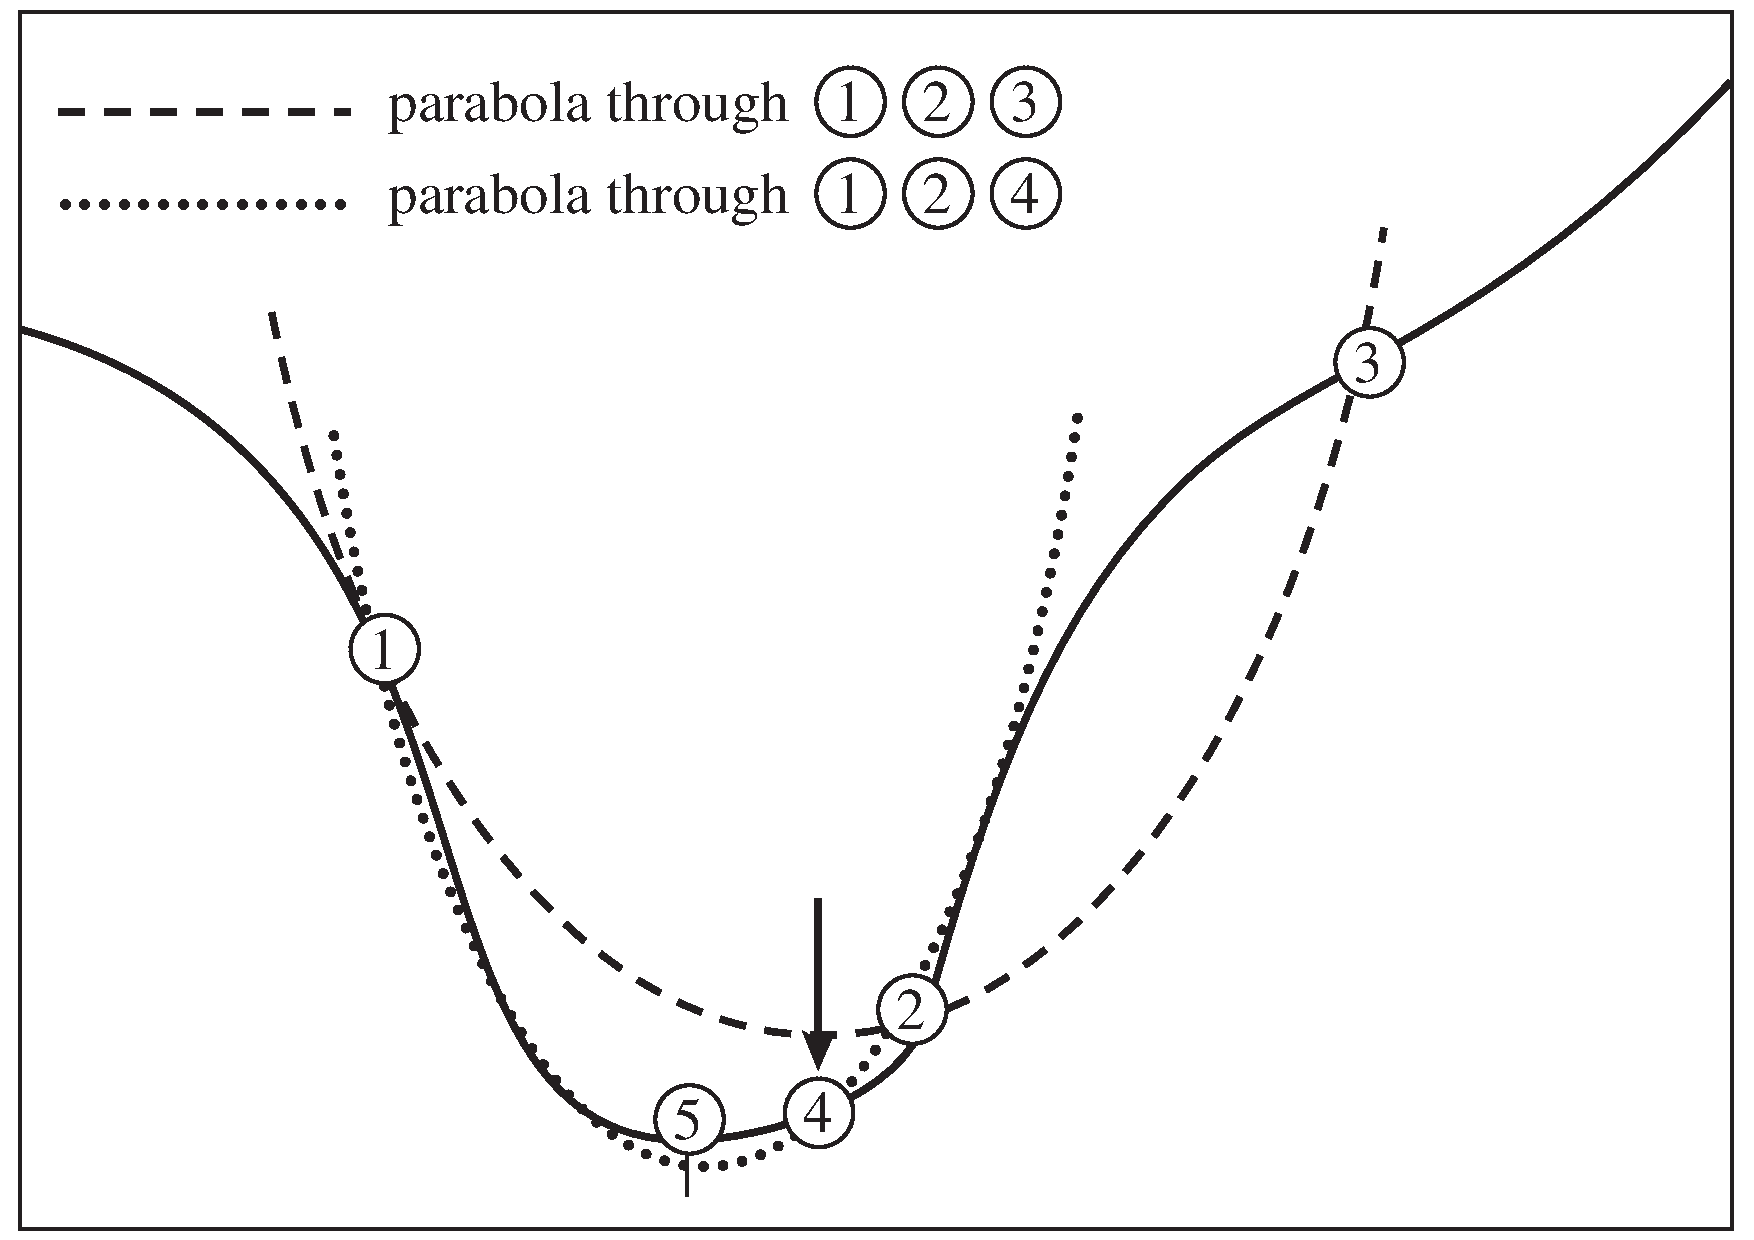
\includegraphics[width=0.75\textwidth]{parabola.pdf}
    \caption{Convergência pelo Método de Brent. Figura retirada de \cite{Brent} }
\label{fig:parabolas}
\end{figure}

A figura \ref{fig:parabolas} mostra duas iterações da interpolação parabólica. É possível notar que a primeira estimativa do minimizador é obtida em $4$ e que, em seguida, esta muda para $5$, se aproximando ainda mais do real valor do minimizador da função $f(x)$.
 
\subsection{Algoritmo}

\vspace{0.5cm}

Durante qualquer fase do algoritmo, este possui um conjunto de 6 pontos $(a, b, u, v, w, x)$. Os pontos $a$ e $b$ definem o intervalo enquadrante de cada iteração; $x$ é o minimizador de $f(x)$ obtido até o momento; $w$ é o ponto de segundo menor valor da função objetivo até o momento e $v$ é o valor anterior de $w$; $u$, por sua vez,  é o ponto onde a função foi avaliada mais recentemente. Um outro ponto que também aparece no algoritmo é o ponto médio entre $a$ e $b$, i.e $x_m$, no entanto, a função objetivo não é avaliada nele.

Se após o passo $d$ da interpolação parabólica, o melhor ponto $x$ pertencer ao intervalo $[a, \, b]$ e, ainda, se o deslocamento provocado por este passo for inferior ao deslocamento provocado na penúltima iteração, significa que $x$ está convergindo e que a interpolação parabólica pode ser usada. Caso alguma dessas condições não seja satisfeita, o passo $d$ é calculado utilizando a razão áurea do maior segmento dentro do intervalo $[a, \,b]$.\\

O algoritmo retoma o início dos cálculos dos novos pontos $(a, b, u, v, w, x)$ até que a tolerância seja atingida ($ |x-x_m| < tol $), alternando,portanto, entre e a interpolação polinomial e o método da razão áurea na determinação dos intervalos para as próximas iterações. O diagrama de fluxo \ref{fig:brentFlow} exemplifica o algoritmo.

 \begin{figure}
 \centering
 \scalebox{1}{\input{brentFlow.tex}}
 \caption{Fluxograma do Método de Interpolação}
 \label{fig:brentFlow}
 \end{figure}

\subsection{Resultado}

O resultado obtido para o método de Brent utilizando a função teste apresentada previamente neste relatório (eq. \ref{eq:func_obj}) pode ser observado na figura \ref{fig:brent}.\\

\begin{figure}[h!]
\centering
\scalebox{1}{\input{./figuras/brent.tex}}
\caption{Tolerância: $\epsilon =  0.01$. Número de iterações: $n = 12$}
\label{fig:brent}
\end{figure}

É interessante notar que a performance foi bem similar ao método da seção áurea já que a tolerância $\epsilon$ escolhida foi a mesma. No entanto, o método de Brent é consideravelmente mais rápido devido à utilizão da interpolação polinomial. Ao passo que foram necessárias 17 iterações para Seção Áurea convergir, somente 12 bastaram para garantir o mesmo resultado usando o método de Brent.}
\caption{Tolerância: $\epsilon =  0.01$. Número de iterações: $n = 12$}
\label{fig:brent}
\end{figure}

É interessante notar que a performance foi bem similar ao método da seção áurea já que a tolerância $\epsilon$ escolhida foi a mesma. No entanto, o método de Brent é consideravelmente mais rápido devido à utilizão da interpolação polinomial. Ao passo que foram necessárias 17 iterações para Seção Áurea convergir, somente 12 bastaram para garantir o mesmo resultado usando o método de Brent.}
\caption{Tolerância: $\epsilon =  0.01$. Número de iterações: $n = 12$}
\label{fig:brent}
\end{figure}

É interessante notar que a performance foi bem similar ao método da seção áurea já que a tolerância $\epsilon$ escolhida foi a mesma. No entanto, o método de Brent é consideravelmente mais rápido devido à utilizão da interpolação polinomial. Ao passo que foram necessárias 17 iterações para Seção Áurea convergir, somente 12 bastaram para garantir o mesmo resultado usando o método de Brent.

\bibliography{bibliografia}
\bibliographystyle{plain}


\end{document}
